\documentclass[twoside]{book}

% Packages required by doxygen
\usepackage{calc}
\usepackage{doxygen}
\usepackage{graphicx}
\usepackage[utf8]{inputenc}
\usepackage{makeidx}
\usepackage{multicol}
\usepackage{multirow}
\usepackage{textcomp}
\usepackage[table]{xcolor}

% Font selection
\usepackage[T1]{fontenc}
\usepackage{mathptmx}
\usepackage[scaled=.90]{helvet}
\usepackage{courier}
\usepackage{amssymb}
\usepackage{sectsty}
\renewcommand{\familydefault}{\sfdefault}
\allsectionsfont{%
  \fontseries{bc}\selectfont%
  \color{darkgray}%
}
\renewcommand{\DoxyLabelFont}{%
  \fontseries{bc}\selectfont%
  \color{darkgray}%
}

% Page & text layout
\usepackage{geometry}
\geometry{%
  a4paper,%
  top=2.5cm,%
  bottom=2.5cm,%
  left=2.5cm,%
  right=2.5cm%
}
\tolerance=750
\hfuzz=15pt
\hbadness=750
\setlength{\emergencystretch}{15pt}
\setlength{\parindent}{0cm}
\setlength{\parskip}{0.2cm}
\makeatletter
\renewcommand{\paragraph}{%
  \@startsection{paragraph}{4}{0ex}{-1.0ex}{1.0ex}{%
    \normalfont\normalsize\bfseries\SS@parafont%
  }%
}
\renewcommand{\subparagraph}{%
  \@startsection{subparagraph}{5}{0ex}{-1.0ex}{1.0ex}{%
    \normalfont\normalsize\bfseries\SS@subparafont%
  }%
}
\makeatother

% Headers & footers
\usepackage{fancyhdr}
\pagestyle{fancyplain}
\fancyhead[LE]{\fancyplain{}{\bfseries\thepage}}
\fancyhead[CE]{\fancyplain{}{}}
\fancyhead[RE]{\fancyplain{}{\bfseries\leftmark}}
\fancyhead[LO]{\fancyplain{}{\bfseries\rightmark}}
\fancyhead[CO]{\fancyplain{}{}}
\fancyhead[RO]{\fancyplain{}{\bfseries\thepage}}
\fancyfoot[LE]{\fancyplain{}{}}
\fancyfoot[CE]{\fancyplain{}{}}
\fancyfoot[RE]{\fancyplain{}{\bfseries\scriptsize Generated on Fri Apr 18 2014 16\-:58\-:43 for A\-W\-E Media Center by Doxygen }}
\fancyfoot[LO]{\fancyplain{}{\bfseries\scriptsize Generated on Fri Apr 18 2014 16\-:58\-:43 for A\-W\-E Media Center by Doxygen }}
\fancyfoot[CO]{\fancyplain{}{}}
\fancyfoot[RO]{\fancyplain{}{}}
\renewcommand{\footrulewidth}{0.4pt}
\renewcommand{\chaptermark}[1]{%
  \markboth{#1}{}%
}
\renewcommand{\sectionmark}[1]{%
  \markright{\thesection\ #1}%
}

% Indices & bibliography
\usepackage{natbib}
\usepackage[titles]{tocloft}
\setcounter{tocdepth}{3}
\setcounter{secnumdepth}{5}
\makeindex

% Hyperlinks (required, but should be loaded last)
\usepackage{ifpdf}
\ifpdf
  \usepackage[pdftex,pagebackref=true]{hyperref}
\else
  \usepackage[ps2pdf,pagebackref=true]{hyperref}
\fi
\hypersetup{%
  colorlinks=true,%
  linkcolor=blue,%
  citecolor=blue,%
  unicode%
}

% Custom commands
\newcommand{\clearemptydoublepage}{%
  \newpage{\pagestyle{empty}\cleardoublepage}%
}


%===== C O N T E N T S =====

\begin{document}

% Titlepage & ToC
\hypersetup{pageanchor=false}
\pagenumbering{roman}
\begin{titlepage}
\vspace*{7cm}
\begin{center}%
{\Large A\-W\-E Media Center \\[1ex]\large 0.\-1 }\\
\vspace*{1cm}
{\large Generated by Doxygen 1.8.6}\\
\vspace*{0.5cm}
{\small Fri Apr 18 2014 16:58:43}\\
\end{center}
\end{titlepage}
\clearemptydoublepage
\tableofcontents
\clearemptydoublepage
\pagenumbering{arabic}
\hypersetup{pageanchor=true}

%--- Begin generated contents ---
\chapter{Main Page}
\label{index}\hypertarget{index}{}A\-W\-E\-M\-C is programmed using C++ and relies on \href{http://www.qt-project.org/>}{\tt Qt}, \href{http://curl.haxx.se/>}{\tt c\-U\-R\-L}, and (eventually) \href{http://www.sfml-dev.org/>}{\tt S\-F\-M\-L}. \href{http://jsoncpp.sourceforge.net/>}{\tt Json\-Cpp} is included in the source code.

There are 7 central concepts you should understand\-:


\begin{DoxyItemize}
\item Media items are organized in a folder structure using J\-S\-O\-N files to hold metadata and such.
\item Media players play media files.
\item Media services are standalone applications, like a web browser, Netflix, or i\-Tunes.
\item Metadata scrapers get relevant information and images for a media item.
\item Media types describe the default metadata values for a collection of items, like Movies or T\-V Shows.
\item Folder generators make a folder structure with organization based on things like Genre for a specific media type. They also use metadata scrapers to collect information about media items to be placed in the folder structure.
\item Skins describe the way the \hyperlink{namespace_u_i}{U\-I} looks and give default images to files.
\end{DoxyItemize}

\subsection*{Namespaces}

There are a few namespaces you should know about\-:


\begin{DoxyItemize}
\item {\ttfamily std} -\/ Well, this one should be obvious.
\item {\ttfamily \hyperlink{namespace_json}{Json}} -\/ This is the namespace for \href{http://jsoncpp.sourceforge.net/>}{\tt Json\-Cpp}.
\item {\ttfamily \hyperlink{namespace_a_w_e}{A\-W\-E}} -\/ All backend classes fall under this namespace.
\item {\ttfamily \hyperlink{namespace_u_i}{U\-I}} -\/ All user interface classes (i.\-e. windows and widgets) fall under this.
\item {\ttfamily T\-C\-O\-M} -\/ My own little colored command line library included with the code for debugging (it will be removed later). 
\end{DoxyItemize}
\chapter{Media Items}
\label{md___users__alex_github__a_w_e_media_center__code_items__r_e_a_d_m_e}
\hypertarget{md___users__alex_github__a_w_e_media_center__code_items__r_e_a_d_m_e}{}
There are three kinds of media items\-:


\begin{DoxyItemize}
\item {\ttfamily Folder}s, which contain other media items.
\item {\ttfamily Media\-File}s, which represent media to be played by a media player.
\item {\ttfamily Media\-Service}s, which represent standalone apps for media.
\end{DoxyItemize}

All media items have relevant metadata and a {\ttfamily \char`\"{}type\char`\"{}}, which is either {\ttfamily \char`\"{}folder\char`\"{}}, {\ttfamily \char`\"{}file\char`\"{}}, or {\ttfamily \char`\"{}service\char`\"{}}. The {\ttfamily metadata} tag is defined in the corresponding media type. Note that there is an item type and a media type, which are two separate things.

\section*{Folders}

{\ttfamily Folder}s are rather self explanatory\-: they contain other items. The J\-S\-O\-N file structure is as follows\-: \begin{DoxyVerb}{
    "type": "folder",

    "metadata": {
        // metadata for the specific media type goes here
    },

    "items": [
        // list of relative paths to the contained items' JSON files
    ]
}
\end{DoxyVerb}


\section*{Media Files}

{\ttfamily Media\-File}s represent a file with a default \href{../player/README.md>}{\tt media player}, as follows\-: \begin{DoxyVerb}{
    "type": "file",

    "metadata": {
        // metadata for the specific media type goes here
    },

    "player": "player name",
}
\end{DoxyVerb}


\section*{Media Services}

Unlike {\ttfamily Folder}s and {\ttfamily Media\-File}s, {\ttfamily Media\-Service}s are not found in the {\ttfamily root} folder. They are found inside the {\ttfamily services} folder. The J\-S\-O\-N file found in {\ttfamily root} is very simple as follows\-: \begin{DoxyVerb}{
    "type": "service",

    "name": "service name"
}
\end{DoxyVerb}


The {\ttfamily \char`\"{}name\char`\"{}} points to the specific service to place in that {\ttfamily Folder}.

Inside of the {\ttfamily services} folder, there are two sub folders\-: {\ttfamily json} and {\ttfamily plugin}.

\subsection*{External J\-S\-O\-N Services}

The {\ttfamily json} folder contains a set of J\-S\-O\-N files that represent external applications to launch. Each of these J\-S\-O\-N files look like this\-: \begin{DoxyVerb}{
    "name": "service name",

    "command": "terminal command to run"
}
\end{DoxyVerb}


\subsection*{Internal Plugin Services}

The {\ttfamily plugin} folder contains a set of J\-S\-O\-N files and associated dynamic libraries. In order to create the plugin you should implement the {\ttfamily Media\-Service} interface. The accompanying J\-S\-O\-N file looks like this\-: \begin{DoxyVerb}{
    "name": "service name",

    "library": "dynamic library file"
}
\end{DoxyVerb}
 
\chapter{Media Players}
\label{md___users__alex_github__a_w_e_media_center__code_player__r_e_a_d_m_e}
\hypertarget{md___users__alex_github__a_w_e_media_center__code_player__r_e_a_d_m_e}{}
Media players play ../items/\-R\-E\-A\-D\-M\-E.md \char`\"{}media files\char`\"{}, using either a terminal command or a plugin.

\section*{External J\-S\-O\-N Players}

The J\-S\-O\-N file for a media player looks like this\-: \begin{DoxyVerb}{
    "name": "player name",

    "program": "program to run",

    "args": "arguments to pass to the program with file references"
}
\end{DoxyVerb}


The file references to {\ttfamily \char`\"{}args\char`\"{}} can be\-: \begin{DoxyVerb}{1} - the absolute path to the media file
\end{DoxyVerb}


\section*{Internal Plugin Players}

Internal media players must implement the {\ttfamily Media\-Player} interface and fill out the accompanying J\-S\-O\-N file\-: \begin{DoxyVerb}{
    "name": "player name",

    "library": "dynamic library file"
} \end{DoxyVerb}
 
\chapter{Metadata Scraping}
\label{md___users__alex_github__a_w_e_media_center__code_scraper__r_e_a_d_m_e}
\hypertarget{md___users__alex_github__a_w_e_media_center__code_scraper__r_e_a_d_m_e}{}
Explanation of the way in which A\-W\-E\-M\-C scrapes metadata for media files.

\section*{The Metadata\-Scraper interface}

There are three steps to all metadata scraping\-:


\begin{DoxyEnumerate}
\item Creating the scraper object\-: this happens at launch.
\item Preparing the scraper\-: this allocates memory to be used by the scraper and sets settings.
\item Scraping for data\-: the data is scraped using whatever method your class defines.
\item Deactivating the scraper\-: the objects allocated in step 2 are now deleted.
\end{DoxyEnumerate}

\subsection*{How to\-: Create Internal Metadata Scrapers using Plugins}

Essentially, you need to implement the {\ttfamily Metadata\-Scraper} interface, which is designed to be used as a plugin. Read the \href{http://qt-project.org/doc/qt-4.8/plugins-howto.html}{\tt how-\/to for Qt plugins} to learn more. You'll need to use \href{http://jsoncpp.sourceforge.net/>}{\tt Json\-Cpp} to write the settings file out.

In addition to creating the plugin, you must make a J\-S\-O\-N settings file. The only required entries in this file are\-: \begin{DoxyVerb}"name": <name of the scraper as it should appear to the user>,
"plugin": <the plugin library file>
\end{DoxyVerb}


You can include other settings in this file if you like; it should automatically be configurable in the main settings pane.

\subsection*{How To\-: Create External Metadata Scrapers using J\-S\-O\-N Files}

Before reading this how-\/to, here is some information you should know\-:


\begin{DoxyItemize}
\item The general format of a J\-S\-O\-N document (see \href{http://www.json.org/}{\tt http\-://www.\-json.\-org/} for more details).
\item The kinds of metadata that A\-W\-E\-M\-C accepts (see \href{../type/README.md>}{\tt Media Types} for details).
\item The way metadata is stored in a media file's J\-S\-O\-N preference file (see \href{../items/README.md>}{\tt Media Items} for details).
\item Qt regular expressions (see \href{http://qt-project.org/doc/qt-5/qregexp.html>}{\tt Q\-Reg\-Exp} for more details).
\end{DoxyItemize}

Note that, although comments are not officially supported by the J\-S\-O\-N file format, they are supported by A\-W\-E\-M\-C's J\-S\-O\-N reader, \href{http://jsoncpp.sourceforge.net/>}{\tt Json\-Cpp}. Standard {\ttfamily // comment} lines work.

\subsubsection*{Introduction to the idea behind J\-S\-O\-N-\/based scrapers}

The central theory behind these so-\/called {\itshape external scrapers} is that all metadata scrapers do basically the same thing\-: retrieve data from formatted files. Sometimes these are X\-M\-L files (e.\-g. .nfo files from X\-B\-M\-C) and sometimes they are web pages (e.\-g. \href{http://www.themoviedb.org/}{\tt http\-://www.\-themoviedb.\-org/}). J\-S\-O\-N-\/based scrapers in A\-W\-E\-M\-C make no distinction between documents hosted on the internet and locally; they are all just text files that the scraper must read to get information about the media. Thus all you have to do to get a piece of information from a file is\-:


\begin{DoxyEnumerate}
\item Get the file to read from.
\item Look for a specific section of text in that file.
\item Take parts of that section of text and assign those values to metadata properties.
\end{DoxyEnumerate}

The implentation if these so-\/called {\itshape procedures} is based on regular expressions and backreferences. The type of regex used is \href{http://qt-project.org/doc/qt-5/qregexp.html>}{\tt Q\-Reg\-Exp}, while the format of the string where backreferences are placed is defined by the {\ttfamily fmt} parameter for the C++ Standard Library's \href{http://www.cplusplus.com/reference/regex/match_replace/}{\tt backref replacement function}.

\subsubsection*{A template for a scraper}

Here is a template for a scraper\-: \begin{DoxyVerb}{
    // The user picks the scraper based on this name
    "name": <name of your scraper>,

    // This scraper is available to scrape metadata for this type of media item
    "type": <the type of media files>,

    // If a single file can have multiple items in it, set this to true.
    // The procedures below will be repeated for every file name match if true,
    // so make sure your filename regex is strict
    "multiple items per file": <true or false>

    // This helps you get information to use, like the name of the media item
    "filename": <regex to get backreferences from the media file path>,

    // If this type is hierarchical, the metadata should be inherited from the parent folder
    "inherited metadata": {
        <this type's property>: <parent type's property>
    }

    // List of procedures to run using the backreferences from "filename"
    "procedures": [
        {
            // Should this be repeated for every match or just one?
            "repeat": <true or false>,

            // Should the user be prompted to choose which match (or matches) to use?
            // Empty string means that the user should not be prompted
            "ask user": <string to prompt user with>,

            // The file to look in; backrefs are replaced
            "look in file": <formatted string with backrefs>,

            // The regex to search for in the above file; backrefs are replaced
            "for": <formatted regex with backrefs>,

            // Set a bunch of properties to backreferences from "for"
            "set properties": {
                <prop>: <value with backrefs>,
                <prop>: <value with backrefs>,
                // More properties...
            }

            // Run a list of sub-procedures using the backreferences from "for"
            "procedures": [...]
        },
        // More procedures...
    ]

    // For properties that contain file paths or are arrays of file paths, sometimes 
    // you want to import the files.
    // This should always be defined to import every file (except the media file);
    // The user can select settings at the launching of the scraper to decide if
    // this should use links to the files or copy the files.
    // you don't get to choose the new names or the location; AWEMC does that for you
    "copy": [
        <prop with file-path value>,
        <prop with file-path value>,
        // More properties...   
    ]

    // These are for files that should always be imported, e.g. internet files
    "force copy": [
        <prop with file-path value>
        // More properties...
    ]
}
\end{DoxyVerb}


Those of you who have read the \href{../type/README.md>}{\tt Media Types explanation} know that some metadata properties are actually objects that contain other metadata properties. In order to access a property held inside of an object, you must use the {\ttfamily .} operator, much like you would in C++. So to set the \char`\"{}default\char`\"{} property of the \char`\"{}icons\char`\"{} object, I would use\-:

\begin{DoxyVerb}"icons.default": <value>
\end{DoxyVerb}


\subsubsection*{Example scrapers}

There are plenty of example scrapers for you to look at in the {\ttfamily scrapers/json} directory in A\-W\-E\-M\-C's root folder. Specifically, {\ttfamily themoviedb.\-json} and {\ttfamily thetvdb.\-json} are included with A\-W\-E\-M\-C and well commented, so if you need a place to start read up on those.

\subsubsection*{Testing your scraper}

If you use the debug build of A\-W\-E\-M\-C you can see if your scraper J\-S\-O\-N is valid in the command line output. You will also be able to see each individual property being set. You should test your scraper thoroughly in this way before recommending it to others. 
\chapter{Media Types}
\label{md___users__alex_github__a_w_e_media_center__code_type__r_e_a_d_m_e}
\hypertarget{md___users__alex_github__a_w_e_media_center__code_type__r_e_a_d_m_e}{}
The information for a media type is kept in a J\-S\-O\-N file\-: \begin{DoxyVerb}{
    "type": <"folder" or "file">,

    "metadata": {
        "type": <type name>,
        "name": "",
        "location": "",

        "description": "",

        "icons": {
            "default": 0,
            "files": []
        },

        "fanarts": {
            "default": 0,
            "files": []
        },

        "details": {
            "_order": [<first detail>, <second detail>, ...],

            <first detail>: <default value>,
            <second detail>: <default value>,
            // more default details attributes
        }
    },

    "matching files": [
        <file expression you could use in terminal>,
        // more file expressions that also match
    ]

    "contains": [
        // nested media types
    ]
}
\end{DoxyVerb}


\section*{Metadata Default Values}

Sometimes, a property cannot be given a value. In these instances, the value should be specified as the default value. Specified by {\ttfamily \char`\"{}\char`\"{}} or {\ttfamily \mbox{[}\mbox{]}}.

A metadata scraper can decide to inherit a property from the parent folder, which is another kind of default property, but that is not explicity defined in type or file J\-S\-O\-N configurations.

\section*{Folder Structure Generation}

\subsection*{Explanation of File Organization}

The {\ttfamily \char`\"{}contains\char`\"{}} tag indicates how the files should be organized by the folder generator. To better explain this, take T\-V episodes. The episodes should be organized by series and then season. So the {\ttfamily \char`\"{}contains\char`\"{}} property of the {\ttfamily \char`\"{}\-T\-V Series\char`\"{}} type would contain the {\ttfamily \char`\"{}\-T\-V Season\char`\"{}} type, which would contain the {\ttfamily \char`\"{}\-T\-V Episode\char`\"{}} type.

Then, when the folder is generated, the folder structure would look like this\-: \begin{DoxyVerb}All Items
├── <name of series>
│   ├── <season #>
│   │   └── <Episodes>
│   └── <season #>
│       └── <Episodes>
└── <name of series>
    ├── <season #>
    │   └── <Episodes>
    └── <season #>
        └── <Episodes>
\end{DoxyVerb}


You can instantiate the sub-\/type only if you so desire. You can instantiate the {\ttfamily \char`\"{}\-T\-V Episode\char`\"{}} type by itself. Because of this, you should list the properties from the hierarchy, like {\ttfamily \char`\"{}\-Season\char`\"{}} and {\ttfamily \char`\"{}\-Series\char`\"{}}, in the {\ttfamily \char`\"{}metadata.\-details\char`\"{}} tag.

\subsection*{Root directories for the type}

In addition to the {\ttfamily All Items} folder described above, there are also folders for every member of {\ttfamily \char`\"{}metadata.\-details\char`\"{}}. If, for example, there were a {\ttfamily \char`\"{}metadata.\-details.\-Genre\char`\"{}}, the following folder structure would be generated\-: \begin{DoxyVerb}Genre
├── Genre Value 1
│   └── Files with that value
└── Genre Value 2
    └── Files with that value
\end{DoxyVerb}


If the detail is a string, integer, or boolean, it is displayed directly as one of the values. If the detail is an array, each element in that array is a value. So if a movie has two directors, {\ttfamily Bob} and {\ttfamily Bill}, that movie appears under both {\ttfamily Bob} and {\ttfamily Bill}. {\ttfamily Bob} and {\ttfamily Bill} are separate folders under the {\ttfamily Director} folder. Also note that the actual property name is {\ttfamily Director(s)}, but the folder name is {\ttfamily Director}. If a section of text is contained in {\ttfamily ()}, {\ttfamily \{\}}, or {\ttfamily \mbox{[}\mbox{]}} in a detail's name, that text along with the {\ttfamily ()}, {\ttfamily \{\}}, or {\ttfamily \mbox{[}\mbox{]}}, is removed. In addition, other special characters that are not allowed in file names are removed individually. When defining a new type, you should name your detail properties carefully to avoid awkward folder names.

All generated folder structures have an {\ttfamily All Items} folder that lists all of the items. 
\chapter{Todo List}
\label{todo}
\hypertarget{todo}{}

\begin{DoxyRefList}
\item[\label{todo__todo000006}%
\hypertarget{todo__todo000006}{}%
Class \hyperlink{class_a_w_e_1_1_global_settings}{A\-W\-E\-:\-:Global\-Settings} ]Skins... 

Get a better folder adding system. 
\item[\label{todo__todo000002}%
\hypertarget{todo__todo000002}{}%
Class \hyperlink{class_a_w_e_1_1_j_s_o_n_scraper}{A\-W\-E\-:\-:J\-S\-O\-N\-Scraper} ]Change {\ttfamily my\-Type} to be the mystical know-\/all configuration object. 
\item[\label{todo__todo000003}%
\hypertarget{todo__todo000003}{}%
Member \hyperlink{class_a_w_e_1_1_j_s_o_n_scraper_afbed287c0fcae8d797552c711854b4e9}{A\-W\-E\-:\-:J\-S\-O\-N\-Scraper\-:\-:scrape\-Data\-For\-File} (Media\-File $\ast$file, bool ask\-User, bool import)]{\ttfamily import} and {\ttfamily ask\-User} 
\item[\label{todo__todo000001}%
\hypertarget{todo__todo000001}{}%
Class \hyperlink{class_a_w_e_1_1_media_player}{A\-W\-E\-:\-:Media\-Player} ]Make plugin interface. 
\end{DoxyRefList}
\chapter{Deprecated List}
\label{deprecated}
\hypertarget{deprecated}{}

\begin{DoxyRefList}
\item[\label{deprecated__deprecated000001}%
\hypertarget{deprecated__deprecated000001}{}%
Member \hyperlink{class_json_1_1_reader_afa4a59e962d23c4d1c38b433fc95eefa}{Json\-:\-:Reader\-:\-:get\-Formated\-Error\-Messages} () const ]Use get\-Formatted\-Error\-Messages() instead (typo fix). 
\end{DoxyRefList}
\chapter{Namespace Index}
\section{Namespace List}
Here is a list of all documented namespaces with brief descriptions\-:\begin{DoxyCompactList}
\item\contentsline{section}{\hyperlink{namespace_a_w_e}{A\-W\-E} \\*Backend for \hyperlink{class_a_w_e_1_1_a_w_e_m_c}{A\-W\-E\-M\-C} }{\pageref{namespace_a_w_e}}{}
\item\contentsline{section}{\hyperlink{namespace_json}{Json} \\*J\-S\-O\-N (Java\-Script Object Notation) }{\pageref{namespace_json}}{}
\item\contentsline{section}{\hyperlink{namespace_u_i}{U\-I} \\*Contains the user interface classes of A\-W\-E\-M\-C }{\pageref{namespace_u_i}}{}
\end{DoxyCompactList}

\chapter{Hierarchical Index}
\section{Class Hierarchy}
This inheritance list is sorted roughly, but not completely, alphabetically\-:\begin{DoxyCompactList}
\item \contentsline{section}{Json\-:\-:Batch\-Allocator$<$ Allocated\-Type, object\-Per\-Allocation $>$}{\pageref{class_json_1_1_batch_allocator}}{}
\item \contentsline{section}{Json\-:\-:Features}{\pageref{class_json_1_1_features}}{}
\item \contentsline{section}{A\-W\-E\-:\-:Global\-Settings}{\pageref{class_a_w_e_1_1_global_settings}}{}
\item \contentsline{section}{A\-W\-E\-:\-:Media\-Item}{\pageref{class_a_w_e_1_1_media_item}}{}
\begin{DoxyCompactList}
\item \contentsline{section}{A\-W\-E\-:\-:Folder}{\pageref{class_a_w_e_1_1_folder}}{}
\item \contentsline{section}{A\-W\-E\-:\-:Media\-File}{\pageref{class_a_w_e_1_1_media_file}}{}
\item \contentsline{section}{A\-W\-E\-:\-:Media\-Service}{\pageref{class_a_w_e_1_1_media_service}}{}
\begin{DoxyCompactList}
\item \contentsline{section}{A\-W\-E\-:\-:J\-S\-O\-N\-Service}{\pageref{class_a_w_e_1_1_j_s_o_n_service}}{}
\end{DoxyCompactList}
\end{DoxyCompactList}
\item \contentsline{section}{A\-W\-E\-:\-:Media\-Player}{\pageref{class_a_w_e_1_1_media_player}}{}
\begin{DoxyCompactList}
\item \contentsline{section}{A\-W\-E\-:\-:J\-S\-O\-N\-Player}{\pageref{class_a_w_e_1_1_j_s_o_n_player}}{}
\end{DoxyCompactList}
\item \contentsline{section}{A\-W\-E\-:\-:Metadata\-Scraper}{\pageref{class_a_w_e_1_1_metadata_scraper}}{}
\begin{DoxyCompactList}
\item \contentsline{section}{A\-W\-E\-:\-:J\-S\-O\-N\-Scraper}{\pageref{class_a_w_e_1_1_j_s_o_n_scraper}}{}
\end{DoxyCompactList}
\item \contentsline{section}{Json\-:\-:Path}{\pageref{class_json_1_1_path}}{}
\item \contentsline{section}{Json\-:\-:Path\-Argument}{\pageref{class_json_1_1_path_argument}}{}
\item \contentsline{section}{Json\-:\-:Reader}{\pageref{class_json_1_1_reader}}{}
\item \contentsline{section}{Json\-:\-:Static\-String}{\pageref{class_json_1_1_static_string}}{}
\item \contentsline{section}{Json\-:\-:Styled\-Stream\-Writer}{\pageref{class_json_1_1_styled_stream_writer}}{}
\item \contentsline{section}{Json\-:\-:Value}{\pageref{class_json_1_1_value}}{}
\item \contentsline{section}{Json\-:\-:Value\-Iterator\-Base}{\pageref{class_json_1_1_value_iterator_base}}{}
\begin{DoxyCompactList}
\item \contentsline{section}{Json\-:\-:Value\-Const\-Iterator}{\pageref{class_json_1_1_value_const_iterator}}{}
\item \contentsline{section}{Json\-:\-:Value\-Iterator}{\pageref{class_json_1_1_value_iterator}}{}
\end{DoxyCompactList}
\item \contentsline{section}{Json\-:\-:Writer}{\pageref{class_json_1_1_writer}}{}
\begin{DoxyCompactList}
\item \contentsline{section}{Json\-:\-:Fast\-Writer}{\pageref{class_json_1_1_fast_writer}}{}
\item \contentsline{section}{Json\-:\-:Styled\-Writer}{\pageref{class_json_1_1_styled_writer}}{}
\end{DoxyCompactList}
\end{DoxyCompactList}

\chapter{Class Index}
\section{Class List}
Here are the classes, structs, unions and interfaces with brief descriptions\-:\begin{DoxyCompactList}
\item\contentsline{section}{\hyperlink{class_a_w_e_1_1_a_w_e_m_c}{A\-W\-E\-::\-A\-W\-E\-M\-C} \\*This holds a few static instances of important classes, like {\ttfamily \hyperlink{class_a_w_e_1_1_global_settings}{A\-W\-E\-::\-Global\-Settings}} and {\ttfamily U\-I\-::\-Delegate} }{\pageref{class_a_w_e_1_1_a_w_e_m_c}}{}
\item\contentsline{section}{\hyperlink{class_json_1_1_batch_allocator}{Json\-::\-Batch\-Allocator$<$ Allocated\-Type, object\-Per\-Allocation $>$} }{\pageref{class_json_1_1_batch_allocator}}{}
\item\contentsline{section}{\hyperlink{struct_json_1_1_batch_allocator_1_1_batch_info}{Json\-::\-Batch\-Allocator$<$ Allocated\-Type, object\-Per\-Allocation $>$\-::\-Batch\-Info} }{\pageref{struct_json_1_1_batch_allocator_1_1_batch_info}}{}
\item\contentsline{section}{\hyperlink{class_t_c_o_m_1_1_color}{T\-C\-O\-M\-::\-Color} \\*Defines a color to be output to a bash terminal window }{\pageref{class_t_c_o_m_1_1_color}}{}
\item\contentsline{section}{\hyperlink{class_t_c_o_m_1_1_column}{T\-C\-O\-M\-::\-Column} \\*Describes a column of colored text that may be placed next to other such columns }{\pageref{class_t_c_o_m_1_1_column}}{}
\item\contentsline{section}{\hyperlink{class_t_c_o_m_1_1_column_group}{T\-C\-O\-M\-::\-Column\-Group} \\*Describes a group of columns to be printed }{\pageref{class_t_c_o_m_1_1_column_group}}{}
\item\contentsline{section}{\hyperlink{class_t_c_o_m_1_1_command}{T\-C\-O\-M\-::\-Command} \\*Defines a general interface for an A\-N\-S\-I escape sequence }{\pageref{class_t_c_o_m_1_1_command}}{}
\item\contentsline{section}{\hyperlink{struct_json_1_1_value_1_1_comment_info}{Json\-::\-Value\-::\-Comment\-Info} }{\pageref{struct_json_1_1_value_1_1_comment_info}}{}
\item\contentsline{section}{\hyperlink{class_a_w_e_1_1_config_file}{A\-W\-E\-::\-Config\-File} \\*Holds the information for a configuration file in an abstract way }{\pageref{class_a_w_e_1_1_config_file}}{}
\item\contentsline{section}{\hyperlink{class_json_1_1_value_1_1_c_z_string}{Json\-::\-Value\-::\-C\-Z\-String} }{\pageref{class_json_1_1_value_1_1_c_z_string}}{}
\item\contentsline{section}{\hyperlink{class_json_1_1_reader_1_1_error_info}{Json\-::\-Reader\-::\-Error\-Info} }{\pageref{class_json_1_1_reader_1_1_error_info}}{}
\item\contentsline{section}{\hyperlink{class_json_1_1_fast_writer}{Json\-::\-Fast\-Writer} \\*Outputs a \hyperlink{class_json_1_1_value}{Value} in \href{http://www.json.org}{\tt J\-S\-O\-N} format without formatting (not human friendly) }{\pageref{class_json_1_1_fast_writer}}{}
\item\contentsline{section}{\hyperlink{class_json_1_1_features}{Json\-::\-Features} \\*Configuration passed to reader and writer. This configuration object can be used to force the \hyperlink{class_json_1_1_reader}{Reader} or \hyperlink{class_json_1_1_writer}{Writer} to behave in a standard conforming way }{\pageref{class_json_1_1_features}}{}
\item\contentsline{section}{\hyperlink{class_a_w_e_1_1_folder}{A\-W\-E\-::\-Folder} \\*A folder that contains {\ttfamily \hyperlink{class_a_w_e_1_1_media_item}{Media\-Item}}s }{\pageref{class_a_w_e_1_1_folder}}{}
\item\contentsline{section}{\hyperlink{class_u_i_1_1_folder_browser}{U\-I\-::\-Folder\-Browser} \\*A window contents pane designed for browsing files }{\pageref{class_u_i_1_1_folder_browser}}{}
\item\contentsline{section}{\hyperlink{class_a_w_e_1_1_folder_generator}{A\-W\-E\-::\-Folder\-Generator} \\*Defines a folder generator for a hierarchical media type }{\pageref{class_a_w_e_1_1_folder_generator}}{}
\item\contentsline{section}{\hyperlink{class_u_i_1_1_folder_pane}{U\-I\-::\-Folder\-Pane} \\*Allows the user to browse through the items of a folder }{\pageref{class_u_i_1_1_folder_pane}}{}
\item\contentsline{section}{\hyperlink{class_a_w_e_1_1_global_settings}{A\-W\-E\-::\-Global\-Settings} \\*Holds the global settings for \hyperlink{class_a_w_e_1_1_a_w_e_m_c}{A\-W\-E\-M\-C} }{\pageref{class_a_w_e_1_1_global_settings}}{}
\item\contentsline{section}{\hyperlink{class_u_i_1_1_image_item_widget}{U\-I\-::\-Image\-Item\-Widget} \\*A {\ttfamily Q\-List\-Widget\-Item} that holds an image }{\pageref{class_u_i_1_1_image_item_widget}}{}
\item\contentsline{section}{\hyperlink{class_u_i_1_1_image_pane}{U\-I\-::\-Image\-Pane} \\*Defines a class that holds icons and fanart images }{\pageref{class_u_i_1_1_image_pane}}{}
\item\contentsline{section}{\hyperlink{class_u_i_1_1_info_pane}{U\-I\-::\-Info\-Pane} \\*Displays the details and description of a media item }{\pageref{class_u_i_1_1_info_pane}}{}
\item\contentsline{section}{\hyperlink{class_u_i_1_1_item_collection_widget}{U\-I\-::\-Item\-Collection\-Widget} \\*An abstract, scrollable collection of item widgets }{\pageref{class_u_i_1_1_item_collection_widget}}{}
\item\contentsline{section}{\hyperlink{class_u_i_1_1_item_grid_widget}{U\-I\-::\-Item\-Grid\-Widget} \\*An item collection based on a grid layout }{\pageref{class_u_i_1_1_item_grid_widget}}{}
\item\contentsline{section}{\hyperlink{class_u_i_1_1_item_list_widget}{U\-I\-::\-Item\-List\-Widget} \\*An item collection based off of lists }{\pageref{class_u_i_1_1_item_list_widget}}{}
\item\contentsline{section}{\hyperlink{class_u_i_1_1_item_widget}{U\-I\-::\-Item\-Widget} \\*Defines an abstract item widget for lists }{\pageref{class_u_i_1_1_item_widget}}{}
\item\contentsline{section}{\hyperlink{class_a_w_e_1_1_j_s_o_n_player}{A\-W\-E\-::\-J\-S\-O\-N\-Player} \\*Represents an external media player designed in a J\-S\-O\-N file }{\pageref{class_a_w_e_1_1_j_s_o_n_player}}{}
\item\contentsline{section}{\hyperlink{class_a_w_e_1_1_j_s_o_n_scraper}{A\-W\-E\-::\-J\-S\-O\-N\-Scraper} \\*A metadata scraper based on J\-S\-O\-N files }{\pageref{class_a_w_e_1_1_j_s_o_n_scraper}}{}
\item\contentsline{section}{\hyperlink{class_a_w_e_1_1_j_s_o_n_service}{A\-W\-E\-::\-J\-S\-O\-N\-Service} \\*An external media service (aka application) described by a J\-S\-O\-N file }{\pageref{class_a_w_e_1_1_j_s_o_n_service}}{}
\item\contentsline{section}{\hyperlink{class_u_i_1_1_main_window}{U\-I\-::\-Main\-Window} \\*The main window of A\-W\-E\-M\-C, which allows the user to browse through the application }{\pageref{class_u_i_1_1_main_window}}{}
\item\contentsline{section}{\hyperlink{class_a_w_e_1_1_media_file}{A\-W\-E\-::\-Media\-File} \\*Represents a media file }{\pageref{class_a_w_e_1_1_media_file}}{}
\item\contentsline{section}{\hyperlink{class_a_w_e_1_1_media_item}{A\-W\-E\-::\-Media\-Item} \\*Represents a media file, folder, or service }{\pageref{class_a_w_e_1_1_media_item}}{}
\item\contentsline{section}{\hyperlink{class_u_i_1_1_media_item_widget}{U\-I\-::\-Media\-Item\-Widget} \\*A list widget class that holds a media item }{\pageref{class_u_i_1_1_media_item_widget}}{}
\item\contentsline{section}{\hyperlink{class_a_w_e_1_1_media_player}{A\-W\-E\-::\-Media\-Player} \\*Represents an abstract media player's functions }{\pageref{class_a_w_e_1_1_media_player}}{}
\item\contentsline{section}{\hyperlink{class_a_w_e_1_1_media_service}{A\-W\-E\-::\-Media\-Service} \\*A media service, which is basically an application with its own media browser }{\pageref{class_a_w_e_1_1_media_service}}{}
\item\contentsline{section}{\hyperlink{class_a_w_e_1_1_metadata_scraper}{A\-W\-E\-::\-Metadata\-Scraper} \\*Defines the general interface for a metadata scraper }{\pageref{class_a_w_e_1_1_metadata_scraper}}{}
\item\contentsline{section}{\hyperlink{class_u_i_1_1_pane}{U\-I\-::\-Pane} \\*A surface representing a pane of widgets }{\pageref{class_u_i_1_1_pane}}{}
\item\contentsline{section}{\hyperlink{class_json_1_1_path}{Json\-::\-Path} \\*Experimental and untested\-: represents a \char`\"{}path\char`\"{} to access a node }{\pageref{class_json_1_1_path}}{}
\item\contentsline{section}{\hyperlink{class_json_1_1_path_argument}{Json\-::\-Path\-Argument} \\*Experimental and untested\-: represents an element of the \char`\"{}path\char`\"{} to access a node }{\pageref{class_json_1_1_path_argument}}{}
\item\contentsline{section}{\hyperlink{structqt__meta__stringdata___a_w_e_____media_item__t}{qt\-\_\-meta\-\_\-stringdata\-\_\-\-A\-W\-E\-\_\-\-\_\-\-Media\-Item\-\_\-t} }{\pageref{structqt__meta__stringdata___a_w_e_____media_item__t}}{}
\item\contentsline{section}{\hyperlink{structqt__meta__stringdata___u_i_____folder_browser__t}{qt\-\_\-meta\-\_\-stringdata\-\_\-\-U\-I\-\_\-\-\_\-\-Folder\-Browser\-\_\-t} }{\pageref{structqt__meta__stringdata___u_i_____folder_browser__t}}{}
\item\contentsline{section}{\hyperlink{structqt__meta__stringdata___u_i_____folder_pane__t}{qt\-\_\-meta\-\_\-stringdata\-\_\-\-U\-I\-\_\-\-\_\-\-Folder\-Pane\-\_\-t} }{\pageref{structqt__meta__stringdata___u_i_____folder_pane__t}}{}
\item\contentsline{section}{\hyperlink{structqt__meta__stringdata___u_i_____image_item_widget__t}{qt\-\_\-meta\-\_\-stringdata\-\_\-\-U\-I\-\_\-\-\_\-\-Image\-Item\-Widget\-\_\-t} }{\pageref{structqt__meta__stringdata___u_i_____image_item_widget__t}}{}
\item\contentsline{section}{\hyperlink{structqt__meta__stringdata___u_i_____image_pane__t}{qt\-\_\-meta\-\_\-stringdata\-\_\-\-U\-I\-\_\-\-\_\-\-Image\-Pane\-\_\-t} }{\pageref{structqt__meta__stringdata___u_i_____image_pane__t}}{}
\item\contentsline{section}{\hyperlink{structqt__meta__stringdata___u_i_____info_pane__t}{qt\-\_\-meta\-\_\-stringdata\-\_\-\-U\-I\-\_\-\-\_\-\-Info\-Pane\-\_\-t} }{\pageref{structqt__meta__stringdata___u_i_____info_pane__t}}{}
\item\contentsline{section}{\hyperlink{structqt__meta__stringdata___u_i_____item_collection_widget__t}{qt\-\_\-meta\-\_\-stringdata\-\_\-\-U\-I\-\_\-\-\_\-\-Item\-Collection\-Widget\-\_\-t} }{\pageref{structqt__meta__stringdata___u_i_____item_collection_widget__t}}{}
\item\contentsline{section}{\hyperlink{structqt__meta__stringdata___u_i_____item_grid_widget__t}{qt\-\_\-meta\-\_\-stringdata\-\_\-\-U\-I\-\_\-\-\_\-\-Item\-Grid\-Widget\-\_\-t} }{\pageref{structqt__meta__stringdata___u_i_____item_grid_widget__t}}{}
\item\contentsline{section}{\hyperlink{structqt__meta__stringdata___u_i_____item_list_widget__t}{qt\-\_\-meta\-\_\-stringdata\-\_\-\-U\-I\-\_\-\-\_\-\-Item\-List\-Widget\-\_\-t} }{\pageref{structqt__meta__stringdata___u_i_____item_list_widget__t}}{}
\item\contentsline{section}{\hyperlink{structqt__meta__stringdata___u_i_____item_widget__t}{qt\-\_\-meta\-\_\-stringdata\-\_\-\-U\-I\-\_\-\-\_\-\-Item\-Widget\-\_\-t} }{\pageref{structqt__meta__stringdata___u_i_____item_widget__t}}{}
\item\contentsline{section}{\hyperlink{structqt__meta__stringdata___u_i_____media_item_widget__t}{qt\-\_\-meta\-\_\-stringdata\-\_\-\-U\-I\-\_\-\-\_\-\-Media\-Item\-Widget\-\_\-t} }{\pageref{structqt__meta__stringdata___u_i_____media_item_widget__t}}{}
\item\contentsline{section}{\hyperlink{structqt__meta__stringdata___u_i_____text_item_widget__t}{qt\-\_\-meta\-\_\-stringdata\-\_\-\-U\-I\-\_\-\-\_\-\-Text\-Item\-Widget\-\_\-t} }{\pageref{structqt__meta__stringdata___u_i_____text_item_widget__t}}{}
\item\contentsline{section}{\hyperlink{class_json_1_1_reader}{Json\-::\-Reader} \\*Unserialize a \href{http://www.json.org}{\tt J\-S\-O\-N} document into a \hyperlink{class_json_1_1_value}{Value} }{\pageref{class_json_1_1_reader}}{}
\item\contentsline{section}{\hyperlink{class_json_1_1_static_string}{Json\-::\-Static\-String} \\*Lightweight wrapper to tag static string }{\pageref{class_json_1_1_static_string}}{}
\item\contentsline{section}{\hyperlink{class_json_1_1_styled_stream_writer}{Json\-::\-Styled\-Stream\-Writer} \\*Writes a \hyperlink{class_json_1_1_value}{Value} in \href{http://www.json.org}{\tt J\-S\-O\-N} format in a human friendly way, to a stream rather than to a string }{\pageref{class_json_1_1_styled_stream_writer}}{}
\item\contentsline{section}{\hyperlink{class_json_1_1_styled_writer}{Json\-::\-Styled\-Writer} \\*Writes a \hyperlink{class_json_1_1_value}{Value} in \href{http://www.json.org}{\tt J\-S\-O\-N} format in a human friendly way }{\pageref{class_json_1_1_styled_writer}}{}
\item\contentsline{section}{\hyperlink{class_u_i_1_1_text_item_widget}{U\-I\-::\-Text\-Item\-Widget} \\*Displays text in a specific font }{\pageref{class_u_i_1_1_text_item_widget}}{}
\item\contentsline{section}{\hyperlink{class_u_i_1_1_text_pane}{U\-I\-::\-Text\-Pane} \\*This class acts as a replacement for {\ttfamily Q\-Label} when text is needed in a particular font }{\pageref{class_u_i_1_1_text_pane}}{}
\item\contentsline{section}{\hyperlink{class_json_1_1_reader_1_1_token}{Json\-::\-Reader\-::\-Token} }{\pageref{class_json_1_1_reader_1_1_token}}{}
\item\contentsline{section}{\hyperlink{class_u_i_1_1_transparent_scroll_area}{U\-I\-::\-Transparent\-Scroll\-Area} \\*Essentially {\ttfamily Q\-Scroll\-Area}, but with a transparent background }{\pageref{class_u_i_1_1_transparent_scroll_area}}{}
\item\contentsline{section}{\hyperlink{class_json_1_1_value}{Json\-::\-Value} \\*Represents a \href{http://www.json.org}{\tt J\-S\-O\-N} value }{\pageref{class_json_1_1_value}}{}
\item\contentsline{section}{\hyperlink{class_json_1_1_value_const_iterator}{Json\-::\-Value\-Const\-Iterator} \\*Const iterator for object and array value }{\pageref{class_json_1_1_value_const_iterator}}{}
\item\contentsline{section}{\hyperlink{union_json_1_1_value_1_1_value_holder}{Json\-::\-Value\-::\-Value\-Holder} }{\pageref{union_json_1_1_value_1_1_value_holder}}{}
\item\contentsline{section}{\hyperlink{class_json_1_1_value_iterator}{Json\-::\-Value\-Iterator} \\*Iterator for object and array value }{\pageref{class_json_1_1_value_iterator}}{}
\item\contentsline{section}{\hyperlink{class_json_1_1_value_iterator_base}{Json\-::\-Value\-Iterator\-Base} \\*Base class for \hyperlink{class_json_1_1_value}{Value} iterators }{\pageref{class_json_1_1_value_iterator_base}}{}
\item\contentsline{section}{\hyperlink{class_u_i_1_1_window_contents}{U\-I\-::\-Window\-Contents} \\*An interface that describes what could be the contents of the main window }{\pageref{class_u_i_1_1_window_contents}}{}
\item\contentsline{section}{\hyperlink{class_json_1_1_writer}{Json\-::\-Writer} \\*Abstract class for writers }{\pageref{class_json_1_1_writer}}{}
\end{DoxyCompactList}

\chapter{Namespace Documentation}
\hypertarget{namespace_a_w_e}{\section{A\-W\-E Namespace Reference}
\label{namespace_a_w_e}\index{A\-W\-E@{A\-W\-E}}
}


Backend for \hyperlink{class_a_w_e_1_1_a_w_e_m_c}{A\-W\-E\-M\-C}.  


\subsection*{Classes}
\begin{DoxyCompactItemize}
\item 
class \hyperlink{class_a_w_e_1_1_folder}{Folder}
\begin{DoxyCompactList}\small\item\em A folder that contains {\ttfamily \hyperlink{class_a_w_e_1_1_media_item}{Media\-Item}}s. \end{DoxyCompactList}\item 
class \hyperlink{class_a_w_e_1_1_j_s_o_n_service}{J\-S\-O\-N\-Service}
\begin{DoxyCompactList}\small\item\em An external media service (aka application) described by a J\-S\-O\-N file. \end{DoxyCompactList}\item 
class \hyperlink{class_a_w_e_1_1_media_file}{Media\-File}
\begin{DoxyCompactList}\small\item\em Represents a media file. \end{DoxyCompactList}\item 
class \hyperlink{class_a_w_e_1_1_media_item}{Media\-Item}
\begin{DoxyCompactList}\small\item\em Represents a media file, folder, or service. \end{DoxyCompactList}\item 
class \hyperlink{class_a_w_e_1_1_media_service}{Media\-Service}
\begin{DoxyCompactList}\small\item\em A media service, which is basically an application with its own media browser. \end{DoxyCompactList}\item 
class \hyperlink{class_a_w_e_1_1_j_s_o_n_player}{J\-S\-O\-N\-Player}
\begin{DoxyCompactList}\small\item\em Represents an external media player designed in a J\-S\-O\-N file. \end{DoxyCompactList}\item 
class \hyperlink{class_a_w_e_1_1_media_player}{Media\-Player}
\begin{DoxyCompactList}\small\item\em Represents an abstract media player's functions. \end{DoxyCompactList}\item 
class \hyperlink{class_a_w_e_1_1_j_s_o_n_scraper}{J\-S\-O\-N\-Scraper}
\begin{DoxyCompactList}\small\item\em A metadata scraper based on J\-S\-O\-N files. \end{DoxyCompactList}\item 
class \hyperlink{class_a_w_e_1_1_metadata_scraper}{Metadata\-Scraper}
\begin{DoxyCompactList}\small\item\em Defines the general interface for a metadata scraper. \end{DoxyCompactList}\item 
class \hyperlink{class_a_w_e_1_1_global_settings}{Global\-Settings}
\begin{DoxyCompactList}\small\item\em Holds the global settings for \hyperlink{class_a_w_e_1_1_a_w_e_m_c}{A\-W\-E\-M\-C}. \end{DoxyCompactList}\item 
class \hyperlink{class_a_w_e_1_1_a_w_e_m_c}{A\-W\-E\-M\-C}
\begin{DoxyCompactList}\small\item\em This holds a few static instances of important classes, like {\ttfamily \hyperlink{class_a_w_e_1_1_global_settings}{A\-W\-E\-::\-Global\-Settings}} and {\ttfamily U\-I\-::\-Delegate}. \end{DoxyCompactList}\item 
class \hyperlink{class_a_w_e_1_1_config_file}{Config\-File}
\begin{DoxyCompactList}\small\item\em Holds the information for a configuration file in an abstract way. \end{DoxyCompactList}\item 
class \hyperlink{class_a_w_e_1_1_folder_generator}{Folder\-Generator}
\begin{DoxyCompactList}\small\item\em Defines a folder generator for a hierarchical media type. \end{DoxyCompactList}\end{DoxyCompactItemize}
\subsection*{Enumerations}
\begin{DoxyCompactItemize}
\item 
enum \hyperlink{namespace_a_w_e_ad175a5b8a86bf7848825c9bd94c41470}{Item\-Type} \{ {\bfseries F\-O\-L\-D\-E\-R\-\_\-\-T\-Y\-P\-E}, 
{\bfseries F\-I\-L\-E\-\_\-\-T\-Y\-P\-E}, 
{\bfseries S\-E\-R\-V\-I\-C\-E\-\_\-\-T\-Y\-P\-E}
 \}
\begin{DoxyCompactList}\small\item\em The type of item. \end{DoxyCompactList}\end{DoxyCompactItemize}


\subsection{Detailed Description}
Backend for \hyperlink{class_a_w_e_1_1_a_w_e_m_c}{A\-W\-E\-M\-C}. 
\hypertarget{namespace_json}{\section{Json Namespace Reference}
\label{namespace_json}\index{Json@{Json}}
}


J\-S\-O\-N (Java\-Script Object Notation).  


\subsection*{Classes}
\begin{DoxyCompactItemize}
\item 
class \hyperlink{class_json_1_1_features}{Features}
\begin{DoxyCompactList}\small\item\em Configuration passed to reader and writer. This configuration object can be used to force the \hyperlink{class_json_1_1_reader}{Reader} or \hyperlink{class_json_1_1_writer}{Writer} to behave in a standard conforming way. \end{DoxyCompactList}\item 
class \hyperlink{class_json_1_1_static_string}{Static\-String}
\begin{DoxyCompactList}\small\item\em Lightweight wrapper to tag static string. \end{DoxyCompactList}\item 
class \hyperlink{class_json_1_1_value}{Value}
\begin{DoxyCompactList}\small\item\em Represents a \href{http://www.json.org}{\tt J\-S\-O\-N} value. \end{DoxyCompactList}\item 
class \hyperlink{class_json_1_1_path_argument}{Path\-Argument}
\begin{DoxyCompactList}\small\item\em Experimental and untested\-: represents an element of the \char`\"{}path\char`\"{} to access a node. \end{DoxyCompactList}\item 
class \hyperlink{class_json_1_1_path}{Path}
\begin{DoxyCompactList}\small\item\em Experimental and untested\-: represents a \char`\"{}path\char`\"{} to access a node. \end{DoxyCompactList}\item 
class \hyperlink{class_json_1_1_value_iterator_base}{Value\-Iterator\-Base}
\begin{DoxyCompactList}\small\item\em base class for \hyperlink{class_json_1_1_value}{Value} iterators. \end{DoxyCompactList}\item 
class \hyperlink{class_json_1_1_value_const_iterator}{Value\-Const\-Iterator}
\begin{DoxyCompactList}\small\item\em const iterator for object and array value. \end{DoxyCompactList}\item 
class \hyperlink{class_json_1_1_value_iterator}{Value\-Iterator}
\begin{DoxyCompactList}\small\item\em Iterator for object and array value. \end{DoxyCompactList}\item 
class \hyperlink{class_json_1_1_reader}{Reader}
\begin{DoxyCompactList}\small\item\em Unserialize a \href{http://www.json.org}{\tt J\-S\-O\-N} document into a \hyperlink{class_json_1_1_value}{Value}. \end{DoxyCompactList}\item 
class \hyperlink{class_json_1_1_writer}{Writer}
\begin{DoxyCompactList}\small\item\em Abstract class for writers. \end{DoxyCompactList}\item 
class \hyperlink{class_json_1_1_fast_writer}{Fast\-Writer}
\begin{DoxyCompactList}\small\item\em Outputs a \hyperlink{class_json_1_1_value}{Value} in \href{http://www.json.org}{\tt J\-S\-O\-N} format without formatting (not human friendly). \end{DoxyCompactList}\item 
class \hyperlink{class_json_1_1_styled_writer}{Styled\-Writer}
\begin{DoxyCompactList}\small\item\em Writes a \hyperlink{class_json_1_1_value}{Value} in \href{http://www.json.org}{\tt J\-S\-O\-N} format in a human friendly way. \end{DoxyCompactList}\item 
class \hyperlink{class_json_1_1_styled_stream_writer}{Styled\-Stream\-Writer}
\begin{DoxyCompactList}\small\item\em Writes a \hyperlink{class_json_1_1_value}{Value} in \href{http://www.json.org}{\tt J\-S\-O\-N} format in a human friendly way, to a stream rather than to a string. \end{DoxyCompactList}\item 
class \hyperlink{class_json_1_1_batch_allocator}{Batch\-Allocator}
\end{DoxyCompactItemize}
\subsection*{Typedefs}
\begin{DoxyCompactItemize}
\item 
\hypertarget{namespace_json_a08122e8005b706d982e48cca1e2119c7}{typedef int {\bfseries Int}}\label{namespace_json_a08122e8005b706d982e48cca1e2119c7}

\item 
\hypertarget{namespace_json_a800fb90eb6ee8d5d62b600c06f87f7d4}{typedef unsigned int {\bfseries U\-Int}}\label{namespace_json_a800fb90eb6ee8d5d62b600c06f87f7d4}

\item 
\hypertarget{namespace_json_ab7b47d2905da3b4ae60e4e800ec9ae5f}{typedef long long int {\bfseries Int64}}\label{namespace_json_ab7b47d2905da3b4ae60e4e800ec9ae5f}

\item 
\hypertarget{namespace_json_a01f20bce8f8229f38ff890168c0e6452}{typedef unsigned long long int {\bfseries U\-Int64}}\label{namespace_json_a01f20bce8f8229f38ff890168c0e6452}

\item 
\hypertarget{namespace_json_a218d880af853ce786cd985e82571d297}{typedef Int64 {\bfseries Largest\-Int}}\label{namespace_json_a218d880af853ce786cd985e82571d297}

\item 
\hypertarget{namespace_json_ae202ecad69725e23443f465e257456d0}{typedef U\-Int64 {\bfseries Largest\-U\-Int}}\label{namespace_json_ae202ecad69725e23443f465e257456d0}

\item 
\hypertarget{namespace_json_a8048e741f2177c3b5d9ede4a5b8c53c2}{typedef unsigned int {\bfseries Array\-Index}}\label{namespace_json_a8048e741f2177c3b5d9ede4a5b8c53c2}

\item 
\hypertarget{namespace_json_a602bcf69c2042fb61c3b243cb16f04ca}{typedef char {\bfseries U\-Int\-To\-String\-Buffer} \mbox{[}\hyperlink{namespace_json_a0c5f614b019f20b4598dcaec09d9e820ae4f2008c7919f20d81286121d1374424}{uint\-To\-String\-Buffer\-Size}\mbox{]}}\label{namespace_json_a602bcf69c2042fb61c3b243cb16f04ca}

\end{DoxyCompactItemize}
\subsection*{Enumerations}
\begin{DoxyCompactItemize}
\item 
enum \hyperlink{namespace_json_a7d654b75c16a57007925868e38212b4e}{Value\-Type} \{ \\*
\hyperlink{namespace_json_a7d654b75c16a57007925868e38212b4ea7d9899633b4409bd3fc107e6737f8391}{null\-Value} = 0, 
\hyperlink{namespace_json_a7d654b75c16a57007925868e38212b4eae5a9d708d5c9e23ae9bf98898522512d}{int\-Value}, 
\hyperlink{namespace_json_a7d654b75c16a57007925868e38212b4eaea788d9a3bb00adc6d68d97d43e1ccd3}{uint\-Value}, 
\hyperlink{namespace_json_a7d654b75c16a57007925868e38212b4eab837c7b869c14d8be712deb45c9e490e}{real\-Value}, 
\\*
\hyperlink{namespace_json_a7d654b75c16a57007925868e38212b4ea804ef857affea2d415843c73f261c258}{string\-Value}, 
\hyperlink{namespace_json_a7d654b75c16a57007925868e38212b4ea14c30dbf4da86f7b809be299f671f7fd}{boolean\-Value}, 
\hyperlink{namespace_json_a7d654b75c16a57007925868e38212b4eadc8f264f36b55b063c78126b335415f4}{array\-Value}, 
\hyperlink{namespace_json_a7d654b75c16a57007925868e38212b4eae8386dcfc36d1ae897745f7b4f77a1f6}{object\-Value}
 \}
\begin{DoxyCompactList}\small\item\em Type of the value held by a Value object. \end{DoxyCompactList}\item 
enum \hyperlink{namespace_json_a4fc417c23905b2ae9e2c47d197a45351}{Comment\-Placement} \{ \hyperlink{namespace_json_a4fc417c23905b2ae9e2c47d197a45351a52f1733775460517b2ea6bedf4906d52}{comment\-Before} = 0, 
\hyperlink{namespace_json_a4fc417c23905b2ae9e2c47d197a45351a008a230a0586de54f30b76afe70fdcfa}{comment\-After\-On\-Same\-Line}, 
\hyperlink{namespace_json_a4fc417c23905b2ae9e2c47d197a45351ac5784ca53b12250888ddb642b06aebef}{comment\-After}, 
{\bfseries number\-Of\-Comment\-Placement}
 \}
\item 
enum \{ \hyperlink{namespace_json_a0c5f614b019f20b4598dcaec09d9e820ae4f2008c7919f20d81286121d1374424}{uint\-To\-String\-Buffer\-Size} = 3$\ast$sizeof(Largest\-U\-Int)+1
 \}
\end{DoxyCompactItemize}
\subsection*{Functions}
\begin{DoxyCompactItemize}
\item 
std\-::istream \& \hyperlink{namespace_json_a4d245ef719cc0853e8e78eb5f99c16e5}{operator$>$$>$} (std\-::istream \&, \hyperlink{class_json_1_1_value}{Value} \&)
\begin{DoxyCompactList}\small\item\em Read from 'sin' into 'root'. \end{DoxyCompactList}\item 
\hypertarget{namespace_json_a5d3eba6789f9a9c1ab563ff8b4a5090f}{std\-::string J\-S\-O\-N\-\_\-\-A\-P\-I {\bfseries value\-To\-String} (Int value)}\label{namespace_json_a5d3eba6789f9a9c1ab563ff8b4a5090f}

\item 
\hypertarget{namespace_json_a4d43b0ff222bd3975bcf1babca0b978f}{std\-::string J\-S\-O\-N\-\_\-\-A\-P\-I {\bfseries value\-To\-String} (U\-Int value)}\label{namespace_json_a4d43b0ff222bd3975bcf1babca0b978f}

\item 
\hypertarget{namespace_json_abd9c650f70d9434f98f9025e2e2faf2d}{std\-::string J\-S\-O\-N\-\_\-\-A\-P\-I {\bfseries value\-To\-String} (Largest\-Int value)}\label{namespace_json_abd9c650f70d9434f98f9025e2e2faf2d}

\item 
\hypertarget{namespace_json_a3f46b0bc62b95a9426a2da0117bdf9f0}{std\-::string J\-S\-O\-N\-\_\-\-A\-P\-I {\bfseries value\-To\-String} (Largest\-U\-Int value)}\label{namespace_json_a3f46b0bc62b95a9426a2da0117bdf9f0}

\item 
\hypertarget{namespace_json_a99995d7dafa4f4970b349d7d3c8d1d99}{std\-::string J\-S\-O\-N\-\_\-\-A\-P\-I {\bfseries value\-To\-String} (double value)}\label{namespace_json_a99995d7dafa4f4970b349d7d3c8d1d99}

\item 
\hypertarget{namespace_json_a979ed531f091985e22f0051cd2a8e341}{std\-::string J\-S\-O\-N\-\_\-\-A\-P\-I {\bfseries value\-To\-String} (bool value)}\label{namespace_json_a979ed531f091985e22f0051cd2a8e341}

\item 
\hypertarget{namespace_json_aa0c8235a4a5c6599da5d3332743db8ac}{std\-::string J\-S\-O\-N\-\_\-\-A\-P\-I {\bfseries value\-To\-Quoted\-String} (const char $\ast$value)}\label{namespace_json_aa0c8235a4a5c6599da5d3332743db8ac}

\item 
std\-::ostream \& \hyperlink{namespace_json_a87bc83d7e90fc666d28aa16727deda2f}{operator$<$$<$} (std\-::ostream \&, const \hyperlink{class_json_1_1_value}{Value} \&root)
\begin{DoxyCompactList}\small\item\em Output using the \hyperlink{class_json_1_1_styled_stream_writer}{Styled\-Stream\-Writer}. \end{DoxyCompactList}\end{DoxyCompactItemize}


\subsection{Detailed Description}
J\-S\-O\-N (Java\-Script Object Notation). 

\subsection{Enumeration Type Documentation}
\hypertarget{namespace_json_a0c5f614b019f20b4598dcaec09d9e820}{\subsubsection[{anonymous enum}]{\setlength{\rightskip}{0pt plus 5cm}anonymous enum}}\label{namespace_json_a0c5f614b019f20b4598dcaec09d9e820}
\begin{Desc}
\item[Enumerator]\par
\begin{description}
\index{uint\-To\-String\-Buffer\-Size@{uint\-To\-String\-Buffer\-Size}!Json@{Json}}\index{Json@{Json}!uint\-To\-String\-Buffer\-Size@{uint\-To\-String\-Buffer\-Size}}\item[{\em 
\hypertarget{namespace_json_a0c5f614b019f20b4598dcaec09d9e820ae4f2008c7919f20d81286121d1374424}{uint\-To\-String\-Buffer\-Size}\label{namespace_json_a0c5f614b019f20b4598dcaec09d9e820ae4f2008c7919f20d81286121d1374424}
}]Constant that specify the size of the buffer that must be passed to uint\-To\-String. \end{description}
\end{Desc}
\hypertarget{namespace_json_a4fc417c23905b2ae9e2c47d197a45351}{\index{Json@{Json}!Comment\-Placement@{Comment\-Placement}}
\index{Comment\-Placement@{Comment\-Placement}!Json@{Json}}
\subsubsection[{Comment\-Placement}]{\setlength{\rightskip}{0pt plus 5cm}enum {\bf Json\-::\-Comment\-Placement}}}\label{namespace_json_a4fc417c23905b2ae9e2c47d197a45351}
\begin{Desc}
\item[Enumerator]\par
\begin{description}
\index{comment\-Before@{comment\-Before}!Json@{Json}}\index{Json@{Json}!comment\-Before@{comment\-Before}}\item[{\em 
\hypertarget{namespace_json_a4fc417c23905b2ae9e2c47d197a45351a52f1733775460517b2ea6bedf4906d52}{comment\-Before}\label{namespace_json_a4fc417c23905b2ae9e2c47d197a45351a52f1733775460517b2ea6bedf4906d52}
}]a comment placed on the line before a value \index{comment\-After\-On\-Same\-Line@{comment\-After\-On\-Same\-Line}!Json@{Json}}\index{Json@{Json}!comment\-After\-On\-Same\-Line@{comment\-After\-On\-Same\-Line}}\item[{\em 
\hypertarget{namespace_json_a4fc417c23905b2ae9e2c47d197a45351a008a230a0586de54f30b76afe70fdcfa}{comment\-After\-On\-Same\-Line}\label{namespace_json_a4fc417c23905b2ae9e2c47d197a45351a008a230a0586de54f30b76afe70fdcfa}
}]a comment just after a value on the same line \index{comment\-After@{comment\-After}!Json@{Json}}\index{Json@{Json}!comment\-After@{comment\-After}}\item[{\em 
\hypertarget{namespace_json_a4fc417c23905b2ae9e2c47d197a45351ac5784ca53b12250888ddb642b06aebef}{comment\-After}\label{namespace_json_a4fc417c23905b2ae9e2c47d197a45351ac5784ca53b12250888ddb642b06aebef}
}]a comment on the line after a value (only make sense for root value) \end{description}
\end{Desc}
\hypertarget{namespace_json_a7d654b75c16a57007925868e38212b4e}{\index{Json@{Json}!Value\-Type@{Value\-Type}}
\index{Value\-Type@{Value\-Type}!Json@{Json}}
\subsubsection[{Value\-Type}]{\setlength{\rightskip}{0pt plus 5cm}enum {\bf Json\-::\-Value\-Type}}}\label{namespace_json_a7d654b75c16a57007925868e38212b4e}


Type of the value held by a \hyperlink{class_json_1_1_value}{Value} object. 

\begin{Desc}
\item[Enumerator]\par
\begin{description}
\index{null\-Value@{null\-Value}!Json@{Json}}\index{Json@{Json}!null\-Value@{null\-Value}}\item[{\em 
\hypertarget{namespace_json_a7d654b75c16a57007925868e38212b4ea7d9899633b4409bd3fc107e6737f8391}{null\-Value}\label{namespace_json_a7d654b75c16a57007925868e38212b4ea7d9899633b4409bd3fc107e6737f8391}
}]'null' value \index{int\-Value@{int\-Value}!Json@{Json}}\index{Json@{Json}!int\-Value@{int\-Value}}\item[{\em 
\hypertarget{namespace_json_a7d654b75c16a57007925868e38212b4eae5a9d708d5c9e23ae9bf98898522512d}{int\-Value}\label{namespace_json_a7d654b75c16a57007925868e38212b4eae5a9d708d5c9e23ae9bf98898522512d}
}]signed integer value \index{uint\-Value@{uint\-Value}!Json@{Json}}\index{Json@{Json}!uint\-Value@{uint\-Value}}\item[{\em 
\hypertarget{namespace_json_a7d654b75c16a57007925868e38212b4eaea788d9a3bb00adc6d68d97d43e1ccd3}{uint\-Value}\label{namespace_json_a7d654b75c16a57007925868e38212b4eaea788d9a3bb00adc6d68d97d43e1ccd3}
}]unsigned integer value \index{real\-Value@{real\-Value}!Json@{Json}}\index{Json@{Json}!real\-Value@{real\-Value}}\item[{\em 
\hypertarget{namespace_json_a7d654b75c16a57007925868e38212b4eab837c7b869c14d8be712deb45c9e490e}{real\-Value}\label{namespace_json_a7d654b75c16a57007925868e38212b4eab837c7b869c14d8be712deb45c9e490e}
}]double value \index{string\-Value@{string\-Value}!Json@{Json}}\index{Json@{Json}!string\-Value@{string\-Value}}\item[{\em 
\hypertarget{namespace_json_a7d654b75c16a57007925868e38212b4ea804ef857affea2d415843c73f261c258}{string\-Value}\label{namespace_json_a7d654b75c16a57007925868e38212b4ea804ef857affea2d415843c73f261c258}
}]U\-T\-F-\/8 string value. \index{boolean\-Value@{boolean\-Value}!Json@{Json}}\index{Json@{Json}!boolean\-Value@{boolean\-Value}}\item[{\em 
\hypertarget{namespace_json_a7d654b75c16a57007925868e38212b4ea14c30dbf4da86f7b809be299f671f7fd}{boolean\-Value}\label{namespace_json_a7d654b75c16a57007925868e38212b4ea14c30dbf4da86f7b809be299f671f7fd}
}]bool value \index{array\-Value@{array\-Value}!Json@{Json}}\index{Json@{Json}!array\-Value@{array\-Value}}\item[{\em 
\hypertarget{namespace_json_a7d654b75c16a57007925868e38212b4eadc8f264f36b55b063c78126b335415f4}{array\-Value}\label{namespace_json_a7d654b75c16a57007925868e38212b4eadc8f264f36b55b063c78126b335415f4}
}]array value (ordered list) \index{object\-Value@{object\-Value}!Json@{Json}}\index{Json@{Json}!object\-Value@{object\-Value}}\item[{\em 
\hypertarget{namespace_json_a7d654b75c16a57007925868e38212b4eae8386dcfc36d1ae897745f7b4f77a1f6}{object\-Value}\label{namespace_json_a7d654b75c16a57007925868e38212b4eae8386dcfc36d1ae897745f7b4f77a1f6}
}]object value (collection of name/value pairs). \end{description}
\end{Desc}


\subsection{Function Documentation}
\hypertarget{namespace_json_a87bc83d7e90fc666d28aa16727deda2f}{\index{Json@{Json}!operator$<$$<$@{operator$<$$<$}}
\index{operator$<$$<$@{operator$<$$<$}!Json@{Json}}
\subsubsection[{operator$<$$<$}]{\setlength{\rightskip}{0pt plus 5cm}std\-::ostream \& Json\-::operator$<$$<$ (
\begin{DoxyParamCaption}
\item[{std\-::ostream \&}]{sout, }
\item[{const Value \&}]{root}
\end{DoxyParamCaption}
)}}\label{namespace_json_a87bc83d7e90fc666d28aa16727deda2f}


Output using the \hyperlink{class_json_1_1_styled_stream_writer}{Styled\-Stream\-Writer}. 

\begin{DoxySeeAlso}{See Also}
\hyperlink{namespace_json_a4d245ef719cc0853e8e78eb5f99c16e5}{Json\-::operator$>$$>$()} 
\end{DoxySeeAlso}
\hypertarget{namespace_json_a4d245ef719cc0853e8e78eb5f99c16e5}{\index{Json@{Json}!operator$>$$>$@{operator$>$$>$}}
\index{operator$>$$>$@{operator$>$$>$}!Json@{Json}}
\subsubsection[{operator$>$$>$}]{\setlength{\rightskip}{0pt plus 5cm}std\-::istream \& Json\-::operator$>$$>$ (
\begin{DoxyParamCaption}
\item[{std\-::istream \&}]{sin, }
\item[{Value \&}]{root}
\end{DoxyParamCaption}
)}}\label{namespace_json_a4d245ef719cc0853e8e78eb5f99c16e5}


Read from 'sin' into 'root'. 

Always keep comments from the input J\-S\-O\-N.

This can be used to read a file into a particular sub-\/object. For example\-: 
\begin{DoxyCode}
\hyperlink{class_json_1_1_value}{Json::Value} root;
cin >> root[\textcolor{stringliteral}{"dir"}][\textcolor{stringliteral}{"file"}];
cout << root;
\end{DoxyCode}
 Result\-: \begin{DoxyVerb}{
"dir": {
    "file": {
    // The input stream JSON would be nested here.
    }
}
}
\end{DoxyVerb}
 
\begin{DoxyExceptions}{Exceptions}
{\em std\-::exception} & on parse error. \\
\hline
\end{DoxyExceptions}
\begin{DoxySeeAlso}{See Also}
\hyperlink{namespace_json_a87bc83d7e90fc666d28aa16727deda2f}{Json\-::operator$<$$<$()} 
\end{DoxySeeAlso}

\chapter{Class Documentation}
\hypertarget{class_json_1_1_batch_allocator}{\section{Json\-:\-:Batch\-Allocator$<$ Allocated\-Type, object\-Per\-Allocation $>$ Class Template Reference}
\label{class_json_1_1_batch_allocator}\index{Json\-::\-Batch\-Allocator$<$ Allocated\-Type, object\-Per\-Allocation $>$@{Json\-::\-Batch\-Allocator$<$ Allocated\-Type, object\-Per\-Allocation $>$}}
}
\subsection*{Classes}
\begin{DoxyCompactItemize}
\item 
struct \hyperlink{struct_json_1_1_batch_allocator_1_1_batch_info}{Batch\-Info}
\end{DoxyCompactItemize}
\subsection*{Public Types}
\begin{DoxyCompactItemize}
\item 
\hypertarget{class_json_1_1_batch_allocator_a031e753885fcb007c20511e15f84d1a4}{typedef Allocated\-Type {\bfseries Type}}\label{class_json_1_1_batch_allocator_a031e753885fcb007c20511e15f84d1a4}

\end{DoxyCompactItemize}
\subsection*{Public Member Functions}
\begin{DoxyCompactItemize}
\item 
\hypertarget{class_json_1_1_batch_allocator_a96aae4d9032847b074e72a0cf32bc9ea}{{\bfseries Batch\-Allocator} (unsigned int objects\-Per\-Page=255)}\label{class_json_1_1_batch_allocator_a96aae4d9032847b074e72a0cf32bc9ea}

\item 
Allocated\-Type $\ast$ \hyperlink{class_json_1_1_batch_allocator_a4909756c2d33bd0f07662e88e4f850dd}{allocate} ()
\item 
void \hyperlink{class_json_1_1_batch_allocator_aceb116aceb6bb5bbcfd05433abc04ba5}{release} (Allocated\-Type $\ast$object)
\end{DoxyCompactItemize}
\subsection*{Private Member Functions}
\begin{DoxyCompactItemize}
\item 
\hypertarget{class_json_1_1_batch_allocator_af240399628f3cf1099ede92ef1ec4274}{{\bfseries Batch\-Allocator} (const \hyperlink{class_json_1_1_batch_allocator}{Batch\-Allocator} \&)}\label{class_json_1_1_batch_allocator_af240399628f3cf1099ede92ef1ec4274}

\item 
\hypertarget{class_json_1_1_batch_allocator_ad2ab8896da0685b6c7eb5f7bfd5304d3}{void {\bfseries operator=} (const \hyperlink{class_json_1_1_batch_allocator}{Batch\-Allocator} \&)}\label{class_json_1_1_batch_allocator_ad2ab8896da0685b6c7eb5f7bfd5304d3}

\end{DoxyCompactItemize}
\subsection*{Static Private Member Functions}
\begin{DoxyCompactItemize}
\item 
\hypertarget{class_json_1_1_batch_allocator_a41f6367bbed5bdf39d2c8dc8f6bbf29d}{static \hyperlink{struct_json_1_1_batch_allocator_1_1_batch_info}{Batch\-Info} $\ast$ {\bfseries allocate\-Batch} (unsigned int objects\-Per\-Page)}\label{class_json_1_1_batch_allocator_a41f6367bbed5bdf39d2c8dc8f6bbf29d}

\end{DoxyCompactItemize}
\subsection*{Private Attributes}
\begin{DoxyCompactItemize}
\item 
\hypertarget{class_json_1_1_batch_allocator_ab96f6d89d8754359cdb59587d8eed5b5}{\hyperlink{struct_json_1_1_batch_allocator_1_1_batch_info}{Batch\-Info} $\ast$ {\bfseries batches\-\_\-}}\label{class_json_1_1_batch_allocator_ab96f6d89d8754359cdb59587d8eed5b5}

\item 
\hypertarget{class_json_1_1_batch_allocator_af300cf30cc086974f34effcc893e8dea}{\hyperlink{struct_json_1_1_batch_allocator_1_1_batch_info}{Batch\-Info} $\ast$ {\bfseries current\-Batch\-\_\-}}\label{class_json_1_1_batch_allocator_af300cf30cc086974f34effcc893e8dea}

\item 
\hypertarget{class_json_1_1_batch_allocator_a7532989b88c9f124f83394f24737378a}{Allocated\-Type $\ast$ \hyperlink{class_json_1_1_batch_allocator_a7532989b88c9f124f83394f24737378a}{free\-Head\-\_\-}}\label{class_json_1_1_batch_allocator_a7532989b88c9f124f83394f24737378a}

\begin{DoxyCompactList}\small\item\em Head of a single linked list within the allocated space of freeed object. \end{DoxyCompactList}\item 
\hypertarget{class_json_1_1_batch_allocator_aa7a906cb96f6c92cb06f519b15539a5c}{unsigned int {\bfseries objects\-Per\-Page\-\_\-}}\label{class_json_1_1_batch_allocator_aa7a906cb96f6c92cb06f519b15539a5c}

\end{DoxyCompactItemize}


\subsection{Member Function Documentation}
\hypertarget{class_json_1_1_batch_allocator_a4909756c2d33bd0f07662e88e4f850dd}{\index{Json\-::\-Batch\-Allocator@{Json\-::\-Batch\-Allocator}!allocate@{allocate}}
\index{allocate@{allocate}!Json::BatchAllocator@{Json\-::\-Batch\-Allocator}}
\subsubsection[{allocate}]{\setlength{\rightskip}{0pt plus 5cm}template$<$typename Allocated\-Type , const unsigned int object\-Per\-Allocation$>$ Allocated\-Type$\ast$ {\bf Json\-::\-Batch\-Allocator}$<$ Allocated\-Type, object\-Per\-Allocation $>$\-::allocate (
\begin{DoxyParamCaption}
{}
\end{DoxyParamCaption}
)\hspace{0.3cm}{\ttfamily [inline]}}}\label{class_json_1_1_batch_allocator_a4909756c2d33bd0f07662e88e4f850dd}
allocate space for an array of object\-Per\-Allocation object. \begin{DoxyWarning}{Warning}
it is the responsability of the caller to call objects constructors. 
\end{DoxyWarning}
\hypertarget{class_json_1_1_batch_allocator_aceb116aceb6bb5bbcfd05433abc04ba5}{\index{Json\-::\-Batch\-Allocator@{Json\-::\-Batch\-Allocator}!release@{release}}
\index{release@{release}!Json::BatchAllocator@{Json\-::\-Batch\-Allocator}}
\subsubsection[{release}]{\setlength{\rightskip}{0pt plus 5cm}template$<$typename Allocated\-Type , const unsigned int object\-Per\-Allocation$>$ void {\bf Json\-::\-Batch\-Allocator}$<$ Allocated\-Type, object\-Per\-Allocation $>$\-::release (
\begin{DoxyParamCaption}
\item[{Allocated\-Type $\ast$}]{object}
\end{DoxyParamCaption}
)\hspace{0.3cm}{\ttfamily [inline]}}}\label{class_json_1_1_batch_allocator_aceb116aceb6bb5bbcfd05433abc04ba5}
Release the object. \begin{DoxyWarning}{Warning}
it is the responsability of the caller to actually destruct the object. 
\end{DoxyWarning}


The documentation for this class was generated from the following file\-:\begin{DoxyCompactItemize}
\item 
/\-Users/\-Alex/github/\-A\-W\-E\-Media\-Center/\-Code/libs/json/jsoncpp.\-cpp\end{DoxyCompactItemize}

\hypertarget{class_json_1_1_fast_writer}{\section{Json\-:\-:Fast\-Writer Class Reference}
\label{class_json_1_1_fast_writer}\index{Json\-::\-Fast\-Writer@{Json\-::\-Fast\-Writer}}
}


Outputs a \hyperlink{class_json_1_1_value}{Value} in \href{http://www.json.org}{\tt J\-S\-O\-N} format without formatting (not human friendly).  




{\ttfamily \#include $<$json.\-h$>$}

Inheritance diagram for Json\-:\-:Fast\-Writer\-:\begin{figure}[H]
\begin{center}
\leavevmode
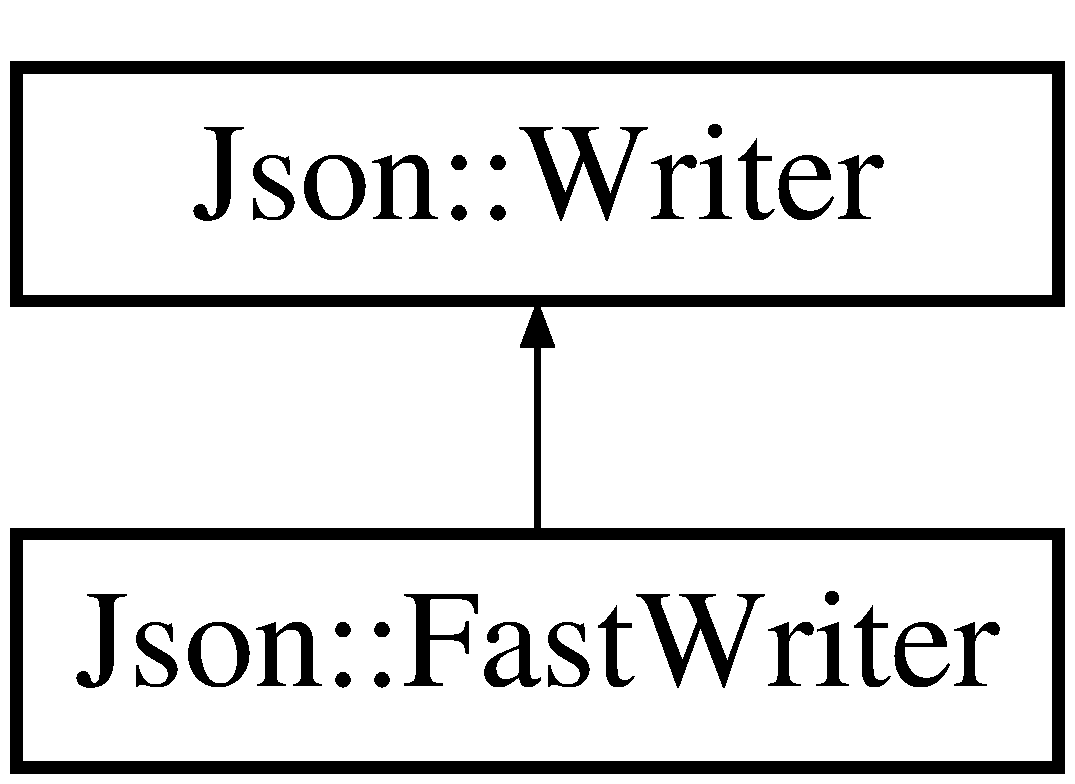
\includegraphics[height=2.000000cm]{class_json_1_1_fast_writer}
\end{center}
\end{figure}
\subsection*{Public Member Functions}
\begin{DoxyCompactItemize}
\item 
\hypertarget{class_json_1_1_fast_writer_a78d98e9f76d33660ad6e6a1abe287d45}{void {\bfseries enable\-Y\-A\-M\-L\-Compatibility} ()}\label{class_json_1_1_fast_writer_a78d98e9f76d33660ad6e6a1abe287d45}

\item 
\hypertarget{class_json_1_1_fast_writer_aa66218a56447222f91d64db618935a19}{virtual std\-::string {\bfseries write} (const \hyperlink{class_json_1_1_value}{Value} \&root)}\label{class_json_1_1_fast_writer_aa66218a56447222f91d64db618935a19}

\end{DoxyCompactItemize}
\subsection*{Private Member Functions}
\begin{DoxyCompactItemize}
\item 
\hypertarget{class_json_1_1_fast_writer_a2ef4a2ce13a341171f01f414f4fdd765}{void {\bfseries write\-Value} (const \hyperlink{class_json_1_1_value}{Value} \&value)}\label{class_json_1_1_fast_writer_a2ef4a2ce13a341171f01f414f4fdd765}

\end{DoxyCompactItemize}
\subsection*{Private Attributes}
\begin{DoxyCompactItemize}
\item 
\hypertarget{class_json_1_1_fast_writer_afc70d465b79bfc7741ff75294dcefeab}{std\-::string {\bfseries document\-\_\-}}\label{class_json_1_1_fast_writer_afc70d465b79bfc7741ff75294dcefeab}

\item 
\hypertarget{class_json_1_1_fast_writer_a4c4c1911179bf472d24492915b0e489a}{bool {\bfseries yaml\-Compatiblity\-Enabled\-\_\-}}\label{class_json_1_1_fast_writer_a4c4c1911179bf472d24492915b0e489a}

\end{DoxyCompactItemize}


\subsection{Detailed Description}
Outputs a \hyperlink{class_json_1_1_value}{Value} in \href{http://www.json.org}{\tt J\-S\-O\-N} format without formatting (not human friendly). 

The J\-S\-O\-N document is written in a single line. It is not intended for 'human' consumption, but may be usefull to support feature such as R\-P\-C where bandwith is limited. \begin{DoxySeeAlso}{See Also}
\hyperlink{class_json_1_1_reader}{Reader}, \hyperlink{class_json_1_1_value}{Value} 
\end{DoxySeeAlso}


The documentation for this class was generated from the following files\-:\begin{DoxyCompactItemize}
\item 
/\-Users/\-Alex/github/\-A\-W\-E\-Media\-Center/\-Code/libs/json/json.\-h\item 
/\-Users/\-Alex/github/\-A\-W\-E\-Media\-Center/\-Code/libs/json/jsoncpp.\-cpp\end{DoxyCompactItemize}

\hypertarget{class_json_1_1_features}{\section{Json\-:\-:Features Class Reference}
\label{class_json_1_1_features}\index{Json\-::\-Features@{Json\-::\-Features}}
}


Configuration passed to reader and writer. This configuration object can be used to force the \hyperlink{class_json_1_1_reader}{Reader} or \hyperlink{class_json_1_1_writer}{Writer} to behave in a standard conforming way.  




{\ttfamily \#include $<$json.\-h$>$}

\subsection*{Public Member Functions}
\begin{DoxyCompactItemize}
\item 
\hypertarget{class_json_1_1_features_ad15a091cb61bb31323299a95970d2644}{\hyperlink{class_json_1_1_features_ad15a091cb61bb31323299a95970d2644}{Features} ()}\label{class_json_1_1_features_ad15a091cb61bb31323299a95970d2644}

\begin{DoxyCompactList}\small\item\em Initialize the configuration like Json\-Config\-::all\-Features;. \end{DoxyCompactList}\end{DoxyCompactItemize}
\subsection*{Static Public Member Functions}
\begin{DoxyCompactItemize}
\item 
static \hyperlink{class_json_1_1_features}{Features} \hyperlink{class_json_1_1_features_a63894da6e2c100b38741fa933f3d33ae}{all} ()
\begin{DoxyCompactList}\small\item\em A configuration that allows all features and assumes all strings are U\-T\-F-\/8. \end{DoxyCompactList}\item 
static \hyperlink{class_json_1_1_features}{Features} \hyperlink{class_json_1_1_features_ae23176c14b2e79e81fb61fb1a8ab58ee}{strict\-Mode} ()
\begin{DoxyCompactList}\small\item\em A configuration that is strictly compatible with the J\-S\-O\-N specification. \end{DoxyCompactList}\end{DoxyCompactItemize}
\subsection*{Public Attributes}
\begin{DoxyCompactItemize}
\item 
\hypertarget{class_json_1_1_features_a33afd389719624b6bdb23950b3c346c9}{bool \hyperlink{class_json_1_1_features_a33afd389719624b6bdb23950b3c346c9}{allow\-Comments\-\_\-}}\label{class_json_1_1_features_a33afd389719624b6bdb23950b3c346c9}

\begin{DoxyCompactList}\small\item\em {\ttfamily true} if comments are allowed. Default\-: {\ttfamily true}. \end{DoxyCompactList}\item 
\hypertarget{class_json_1_1_features_a1162c37a1458adc32582b585b552f9c3}{bool \hyperlink{class_json_1_1_features_a1162c37a1458adc32582b585b552f9c3}{strict\-Root\-\_\-}}\label{class_json_1_1_features_a1162c37a1458adc32582b585b552f9c3}

\begin{DoxyCompactList}\small\item\em {\ttfamily true} if root must be either an array or an object value. Default\-: {\ttfamily false}. \end{DoxyCompactList}\end{DoxyCompactItemize}


\subsection{Detailed Description}
Configuration passed to reader and writer. This configuration object can be used to force the \hyperlink{class_json_1_1_reader}{Reader} or \hyperlink{class_json_1_1_writer}{Writer} to behave in a standard conforming way. 

\subsection{Member Function Documentation}
\hypertarget{class_json_1_1_features_a63894da6e2c100b38741fa933f3d33ae}{\index{Json\-::\-Features@{Json\-::\-Features}!all@{all}}
\index{all@{all}!Json::Features@{Json\-::\-Features}}
\subsubsection[{all}]{\setlength{\rightskip}{0pt plus 5cm}{\bf Features} Json\-::\-Features\-::all (
\begin{DoxyParamCaption}
{}
\end{DoxyParamCaption}
)\hspace{0.3cm}{\ttfamily [static]}}}\label{class_json_1_1_features_a63894da6e2c100b38741fa933f3d33ae}


A configuration that allows all features and assumes all strings are U\-T\-F-\/8. 


\begin{DoxyItemize}
\item C \& C++ comments are allowed
\item Root object can be any J\-S\-O\-N value
\item Assumes \hyperlink{class_json_1_1_value}{Value} strings are encoded in U\-T\-F-\/8 
\end{DoxyItemize}\hypertarget{class_json_1_1_features_ae23176c14b2e79e81fb61fb1a8ab58ee}{\index{Json\-::\-Features@{Json\-::\-Features}!strict\-Mode@{strict\-Mode}}
\index{strict\-Mode@{strict\-Mode}!Json::Features@{Json\-::\-Features}}
\subsubsection[{strict\-Mode}]{\setlength{\rightskip}{0pt plus 5cm}{\bf Features} Json\-::\-Features\-::strict\-Mode (
\begin{DoxyParamCaption}
{}
\end{DoxyParamCaption}
)\hspace{0.3cm}{\ttfamily [static]}}}\label{class_json_1_1_features_ae23176c14b2e79e81fb61fb1a8ab58ee}


A configuration that is strictly compatible with the J\-S\-O\-N specification. 


\begin{DoxyItemize}
\item Comments are forbidden.
\item Root object must be either an array or an object value.
\item Assumes \hyperlink{class_json_1_1_value}{Value} strings are encoded in U\-T\-F-\/8 
\end{DoxyItemize}

The documentation for this class was generated from the following files\-:\begin{DoxyCompactItemize}
\item 
/\-Users/\-Alex/github/\-A\-W\-E\-Media\-Center/\-Code/libs/json/json.\-h\item 
/\-Users/\-Alex/github/\-A\-W\-E\-Media\-Center/\-Code/libs/json/jsoncpp.\-cpp\end{DoxyCompactItemize}

\hypertarget{class_a_w_e_1_1_folder}{\section{A\-W\-E\-:\-:Folder Class Reference}
\label{class_a_w_e_1_1_folder}\index{A\-W\-E\-::\-Folder@{A\-W\-E\-::\-Folder}}
}


A folder that contains {\ttfamily \hyperlink{class_a_w_e_1_1_media_item}{Media\-Item}}s.  




{\ttfamily \#include $<$A\-W\-E\-Folder.\-h$>$}

Inheritance diagram for A\-W\-E\-:\-:Folder\-:\begin{figure}[H]
\begin{center}
\leavevmode
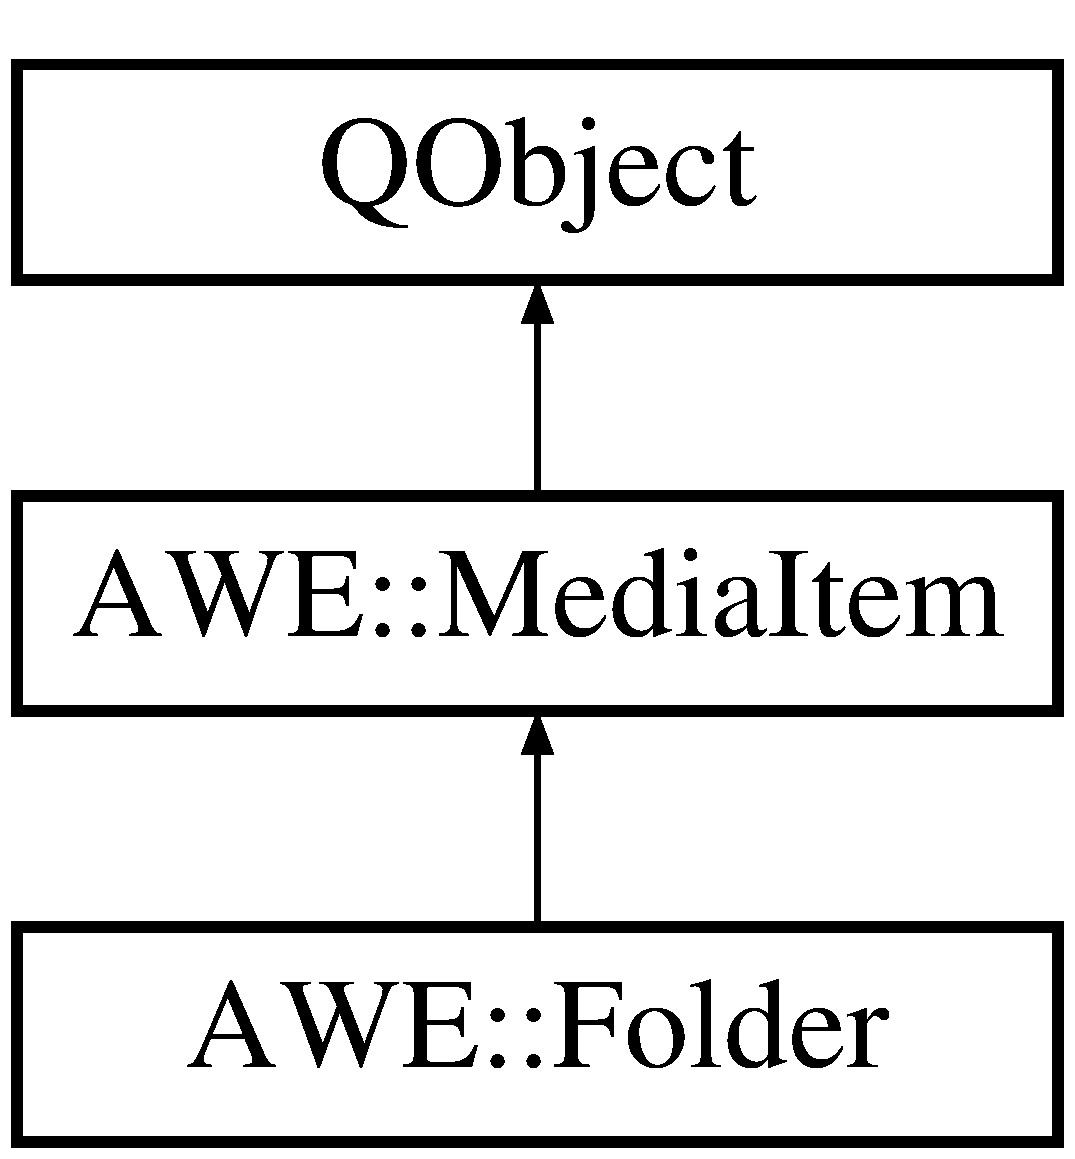
\includegraphics[height=3.000000cm]{class_a_w_e_1_1_folder}
\end{center}
\end{figure}
\subsection*{Public Member Functions}
\begin{DoxyCompactItemize}
\item 
\hyperlink{class_a_w_e_1_1_folder_aee5d9308a9e516eb913e419c24248810}{Folder} (Q\-Dir folder)
\begin{DoxyCompactList}\small\item\em Construct from the folder's settings. \end{DoxyCompactList}\item 
\hypertarget{class_a_w_e_1_1_folder_a7b9eaf0f340d5275809494685b0a3e1d}{virtual \hyperlink{class_a_w_e_1_1_folder_a7b9eaf0f340d5275809494685b0a3e1d}{$\sim$\-Folder} ()}\label{class_a_w_e_1_1_folder_a7b9eaf0f340d5275809494685b0a3e1d}

\begin{DoxyCompactList}\small\item\em Deconstructor. \end{DoxyCompactList}\item 
virtual \hyperlink{namespace_a_w_e_ad175a5b8a86bf7848825c9bd94c41470}{Item\-Type} \hyperlink{class_a_w_e_1_1_folder_a315c0a52f6e37b357d5f0e4fc5526d52}{get\-Item\-Type} () const 
\begin{DoxyCompactList}\small\item\em Determine the basic type (folder, file, service) \end{DoxyCompactList}\item 
virtual Q\-List$<$ \hyperlink{class_a_w_e_1_1_media_item}{Media\-Item} $\ast$ $>$ \hyperlink{class_a_w_e_1_1_folder_ae5e4053b40082661ad5debf17cbe64ca}{get\-Items} ()
\begin{DoxyCompactList}\small\item\em Get a list of all of the items this folder contains. \end{DoxyCompactList}\item 
virtual void \hyperlink{class_a_w_e_1_1_folder_adb8c48413775f2a23a8107596d617a9d}{add\-Item} (\hyperlink{class_a_w_e_1_1_media_item}{Media\-Item} $\ast$item)
\begin{DoxyCompactList}\small\item\em Add an item. \end{DoxyCompactList}\end{DoxyCompactItemize}
\subsection*{Private Attributes}
\begin{DoxyCompactItemize}
\item 
\hypertarget{class_a_w_e_1_1_folder_a25f0aa0adf40e5deea27e82c06fa29ea}{Q\-List$<$ \hyperlink{class_a_w_e_1_1_media_item}{Media\-Item} $\ast$ $>$ \hyperlink{class_a_w_e_1_1_folder_a25f0aa0adf40e5deea27e82c06fa29ea}{my\-Items}}\label{class_a_w_e_1_1_folder_a25f0aa0adf40e5deea27e82c06fa29ea}

\begin{DoxyCompactList}\small\item\em List of contained items. \end{DoxyCompactList}\end{DoxyCompactItemize}
\subsection*{Additional Inherited Members}


\subsection{Detailed Description}
A folder that contains {\ttfamily \hyperlink{class_a_w_e_1_1_media_item}{Media\-Item}}s. 

\subsection{Constructor \& Destructor Documentation}
\hypertarget{class_a_w_e_1_1_folder_aee5d9308a9e516eb913e419c24248810}{\index{A\-W\-E\-::\-Folder@{A\-W\-E\-::\-Folder}!Folder@{Folder}}
\index{Folder@{Folder}!AWE::Folder@{A\-W\-E\-::\-Folder}}
\subsubsection[{Folder}]{\setlength{\rightskip}{0pt plus 5cm}Folder\-::\-Folder (
\begin{DoxyParamCaption}
\item[{Q\-Dir}]{folder}
\end{DoxyParamCaption}
)}}\label{class_a_w_e_1_1_folder_aee5d9308a9e516eb913e419c24248810}


Construct from the folder's settings. 


\begin{DoxyParams}{Parameters}
{\em folder} & The configuration file for this folder. \\
\hline
\end{DoxyParams}


\subsection{Member Function Documentation}
\hypertarget{class_a_w_e_1_1_folder_adb8c48413775f2a23a8107596d617a9d}{\index{A\-W\-E\-::\-Folder@{A\-W\-E\-::\-Folder}!add\-Item@{add\-Item}}
\index{add\-Item@{add\-Item}!AWE::Folder@{A\-W\-E\-::\-Folder}}
\subsubsection[{add\-Item}]{\setlength{\rightskip}{0pt plus 5cm}void Folder\-::add\-Item (
\begin{DoxyParamCaption}
\item[{{\bf Media\-Item} $\ast$}]{item}
\end{DoxyParamCaption}
)\hspace{0.3cm}{\ttfamily [virtual]}}}\label{class_a_w_e_1_1_folder_adb8c48413775f2a23a8107596d617a9d}


Add an item. 


\begin{DoxyParams}{Parameters}
{\em item} & The item to add to this {\ttfamily \hyperlink{class_a_w_e_1_1_folder}{Folder}}. \\
\hline
\end{DoxyParams}
\hypertarget{class_a_w_e_1_1_folder_ae5e4053b40082661ad5debf17cbe64ca}{\index{A\-W\-E\-::\-Folder@{A\-W\-E\-::\-Folder}!get\-Items@{get\-Items}}
\index{get\-Items@{get\-Items}!AWE::Folder@{A\-W\-E\-::\-Folder}}
\subsubsection[{get\-Items}]{\setlength{\rightskip}{0pt plus 5cm}Q\-List$<$ {\bf Media\-Item} $\ast$ $>$ Folder\-::get\-Items (
\begin{DoxyParamCaption}
{}
\end{DoxyParamCaption}
)\hspace{0.3cm}{\ttfamily [virtual]}}}\label{class_a_w_e_1_1_folder_ae5e4053b40082661ad5debf17cbe64ca}


Get a list of all of the items this folder contains. 

\begin{DoxyReturn}{Returns}
All of the items this folder contains. 
\end{DoxyReturn}
\hypertarget{class_a_w_e_1_1_folder_a315c0a52f6e37b357d5f0e4fc5526d52}{\index{A\-W\-E\-::\-Folder@{A\-W\-E\-::\-Folder}!get\-Item\-Type@{get\-Item\-Type}}
\index{get\-Item\-Type@{get\-Item\-Type}!AWE::Folder@{A\-W\-E\-::\-Folder}}
\subsubsection[{get\-Item\-Type}]{\setlength{\rightskip}{0pt plus 5cm}{\bf Item\-Type} Folder\-::get\-Item\-Type (
\begin{DoxyParamCaption}
{}
\end{DoxyParamCaption}
) const\hspace{0.3cm}{\ttfamily [virtual]}}}\label{class_a_w_e_1_1_folder_a315c0a52f6e37b357d5f0e4fc5526d52}


Determine the basic type (folder, file, service) 

\begin{DoxyReturn}{Returns}
The basic type of this item. 
\end{DoxyReturn}


Implements \hyperlink{class_a_w_e_1_1_media_item_ad7a7ef28069986fad8b2be060fef6e48}{A\-W\-E\-::\-Media\-Item}.



The documentation for this class was generated from the following files\-:\begin{DoxyCompactItemize}
\item 
/\-Users/\-Alex/github/\-A\-W\-E\-Media\-Center/\-Code/items/A\-W\-E\-Folder.\-h\item 
/\-Users/\-Alex/github/\-A\-W\-E\-Media\-Center/\-Code/items/A\-W\-E\-Folder.\-cpp\end{DoxyCompactItemize}

\hypertarget{class_a_w_e_1_1_global_settings}{\section{A\-W\-E\-:\-:Global\-Settings Class Reference}
\label{class_a_w_e_1_1_global_settings}\index{A\-W\-E\-::\-Global\-Settings@{A\-W\-E\-::\-Global\-Settings}}
}


Holds the global settings for A\-W\-E\-M\-C.  




{\ttfamily \#include $<$A\-W\-E\-Global\-Settings.\-h$>$}

\subsection*{Public Types}
\begin{DoxyCompactItemize}
\item 
\hypertarget{class_a_w_e_1_1_global_settings_a45df15954e36fb1bad5385f5249c408e}{typedef std\-::set$<$ std\-::string $>$ \hyperlink{class_a_w_e_1_1_global_settings_a45df15954e36fb1bad5385f5249c408e}{Name\-Set}}\label{class_a_w_e_1_1_global_settings_a45df15954e36fb1bad5385f5249c408e}

\begin{DoxyCompactList}\small\item\em The set type used to hold names. \end{DoxyCompactList}\end{DoxyCompactItemize}
\subsection*{Public Member Functions}
\begin{DoxyCompactItemize}
\item 
\hyperlink{class_a_w_e_1_1_global_settings_a8aa60ae622af94d79cba5321fb0a2816}{Global\-Settings} (const std\-::string \&settings\-File)
\begin{DoxyCompactList}\small\item\em Create the global settings object. \end{DoxyCompactList}\item 
\hyperlink{class_a_w_e_1_1_global_settings_ad3e8fa5120473c6c0151573ad81e1b04}{$\sim$\-Global\-Settings} ()
\begin{DoxyCompactList}\small\item\em Deconstructor. \end{DoxyCompactList}\item 
\hyperlink{class_a_w_e_1_1_metadata_scraper}{Metadata\-Scraper} $\ast$ \hyperlink{class_a_w_e_1_1_global_settings_a40bfab45d901e7c1acdd2d0a8700fd69}{get\-Scraper\-By\-Name} (const std\-::string \&name)
\begin{DoxyCompactList}\small\item\em Get a metadata scraper by name. \end{DoxyCompactList}\item 
\hyperlink{class_json_1_1_value}{Json\-::\-Value} \& \hyperlink{class_a_w_e_1_1_global_settings_a45d865b8b7242f17ad6e83ff014ee4c6}{get\-Scraper\-Settings\-By\-Name} (const std\-::string \&name)
\begin{DoxyCompactList}\small\item\em Get a metadata scraper's settings by name. \end{DoxyCompactList}\item 
const \hyperlink{class_a_w_e_1_1_global_settings_a45df15954e36fb1bad5385f5249c408e}{Name\-Set} \& \hyperlink{class_a_w_e_1_1_global_settings_ac1824eeb7c6319dda29aa061dd13184c}{get\-All\-Metadata\-Scraper\-Names} ()
\begin{DoxyCompactList}\small\item\em Get a set of all metadata scrapers. \end{DoxyCompactList}\item 
\hyperlink{class_a_w_e_1_1_media_player}{Media\-Player} $\ast$ \hyperlink{class_a_w_e_1_1_global_settings_ae2cc7da9b20e508de12f472ba86cf351}{get\-Player\-By\-Name} (const std\-::string \&name)
\begin{DoxyCompactList}\small\item\em Get a media player by name. \end{DoxyCompactList}\item 
\hyperlink{class_json_1_1_value}{Json\-::\-Value} \& \hyperlink{class_a_w_e_1_1_global_settings_a27fbf04ccbc5fb4bf42db0412ff2ab23}{get\-Player\-Settings\-By\-Name} (const std\-::string \&name)
\begin{DoxyCompactList}\small\item\em Get a media player's settings by name. \end{DoxyCompactList}\item 
const \hyperlink{class_a_w_e_1_1_global_settings_a45df15954e36fb1bad5385f5249c408e}{Name\-Set} \& \hyperlink{class_a_w_e_1_1_global_settings_a0fb7bb8eba01fa51841a827741a0731a}{get\-All\-Media\-Player\-Names} ()
\begin{DoxyCompactList}\small\item\em Get a set of all media players. \end{DoxyCompactList}\item 
\hyperlink{class_json_1_1_value}{Json\-::\-Value} \& \hyperlink{class_a_w_e_1_1_global_settings_ab7026bd5fdd6c7b566a1d5c71ef4b21e}{get\-Type\-By\-Name} (const std\-::string \&name)
\begin{DoxyCompactList}\small\item\em Get the media type with the given name. \end{DoxyCompactList}\item 
const \hyperlink{class_a_w_e_1_1_global_settings_a45df15954e36fb1bad5385f5249c408e}{Name\-Set} \& \hyperlink{class_a_w_e_1_1_global_settings_a4104e5ab20b0e63eccc887ef84d8581f}{get\-All\-Media\-Type\-Names} ()
\begin{DoxyCompactList}\small\item\em Get a set of all media types. \end{DoxyCompactList}\item 
const \hyperlink{class_a_w_e_1_1_global_settings_a45df15954e36fb1bad5385f5249c408e}{Name\-Set} \& \hyperlink{class_a_w_e_1_1_global_settings_a836c7a1e4d711e64fcc87b2908a2eb4e}{get\-All\-Media\-Service\-Names} ()
\begin{DoxyCompactList}\small\item\em Get the names of all of the media services. \end{DoxyCompactList}\item 
\hyperlink{class_a_w_e_1_1_media_service}{Media\-Service} $\ast$ \hyperlink{class_a_w_e_1_1_global_settings_ad0d26204fee1973539c9a6962ea9f462}{get\-Media\-Service\-By\-Name} (const std\-::string \&name)
\begin{DoxyCompactList}\small\item\em Get a media service by name. \end{DoxyCompactList}\item 
\hyperlink{class_a_w_e_1_1_media_item}{Media\-Item} $\ast$ \hyperlink{class_a_w_e_1_1_global_settings_ab13f95f4967f7058de61199ad48626ed}{get\-Media\-Item\-By\-J\-S\-O\-N\-File} (const Q\-Dir \&file)
\begin{DoxyCompactList}\small\item\em Get a media item from its J\-S\-O\-N file. \end{DoxyCompactList}\item 
void \hyperlink{class_a_w_e_1_1_global_settings_ac776a76c7c09678fa753e6561cafeda2}{add\-Folder} (const std\-::string \&path, \hyperlink{class_a_w_e_1_1_folder}{Folder} $\ast$folder)
\begin{DoxyCompactList}\small\item\em Add the given folder. \end{DoxyCompactList}\item 
\hyperlink{class_a_w_e_1_1_folder}{Folder} $\ast$ \hyperlink{class_a_w_e_1_1_global_settings_a958723c6d73aa7ab7574ba4c31675e5d}{get\-Root\-Folder} ()
\begin{DoxyCompactList}\small\item\em Get the root folder. \end{DoxyCompactList}\end{DoxyCompactItemize}
\subsection*{Static Public Attributes}
\begin{DoxyCompactItemize}
\item 
\hypertarget{class_a_w_e_1_1_global_settings_a4df7847cd94fe68cf28382f70eedb0b2}{static \hyperlink{class_json_1_1_value}{Json\-::\-Value} {\bfseries null} = Value\-::null}\label{class_a_w_e_1_1_global_settings_a4df7847cd94fe68cf28382f70eedb0b2}

\end{DoxyCompactItemize}


\subsection{Detailed Description}
Holds the global settings for A\-W\-E\-M\-C. 

\begin{DoxyRefDesc}{Todo}
\item[\hyperlink{todo__todo000006}{Todo}]Skins... 

Get a better folder adding system.\end{DoxyRefDesc}


Functions for pretty much anything you want to know about the prefernces for A\-W\-E\-M\-C are here. Every plugin extending A\-W\-E\-M\-C has its own configuration file, which is held in here via sub-\/configuration objects.

You shouldn't need to instantiate this class on your own; most objects are passed a copy of the settings object during creation or through some other means. 

\subsection{Constructor \& Destructor Documentation}
\hypertarget{class_a_w_e_1_1_global_settings_a8aa60ae622af94d79cba5321fb0a2816}{\index{A\-W\-E\-::\-Global\-Settings@{A\-W\-E\-::\-Global\-Settings}!Global\-Settings@{Global\-Settings}}
\index{Global\-Settings@{Global\-Settings}!AWE::GlobalSettings@{A\-W\-E\-::\-Global\-Settings}}
\subsubsection[{Global\-Settings}]{\setlength{\rightskip}{0pt plus 5cm}Global\-Settings\-::\-Global\-Settings (
\begin{DoxyParamCaption}
\item[{const std\-::string \&}]{settings\-File}
\end{DoxyParamCaption}
)}}\label{class_a_w_e_1_1_global_settings_a8aa60ae622af94d79cba5321fb0a2816}


Create the global settings object. 


\begin{DoxyParams}[1]{Parameters}
\mbox{\tt in}  & {\em settings\-File} & The file that contains the settings for A\-W\-E\-M\-C (usually {\ttfamily settings.\-json} in the root folder) \\
\hline
\end{DoxyParams}
\hypertarget{class_a_w_e_1_1_global_settings_ad3e8fa5120473c6c0151573ad81e1b04}{\index{A\-W\-E\-::\-Global\-Settings@{A\-W\-E\-::\-Global\-Settings}!$\sim$\-Global\-Settings@{$\sim$\-Global\-Settings}}
\index{$\sim$\-Global\-Settings@{$\sim$\-Global\-Settings}!AWE::GlobalSettings@{A\-W\-E\-::\-Global\-Settings}}
\subsubsection[{$\sim$\-Global\-Settings}]{\setlength{\rightskip}{0pt plus 5cm}Global\-Settings\-::$\sim$\-Global\-Settings (
\begin{DoxyParamCaption}
{}
\end{DoxyParamCaption}
)}}\label{class_a_w_e_1_1_global_settings_ad3e8fa5120473c6c0151573ad81e1b04}


Deconstructor. 

Deletes every scraper, player and item. 

\subsection{Member Function Documentation}
\hypertarget{class_a_w_e_1_1_global_settings_ac776a76c7c09678fa753e6561cafeda2}{\index{A\-W\-E\-::\-Global\-Settings@{A\-W\-E\-::\-Global\-Settings}!add\-Folder@{add\-Folder}}
\index{add\-Folder@{add\-Folder}!AWE::GlobalSettings@{A\-W\-E\-::\-Global\-Settings}}
\subsubsection[{add\-Folder}]{\setlength{\rightskip}{0pt plus 5cm}void Global\-Settings\-::add\-Folder (
\begin{DoxyParamCaption}
\item[{const std\-::string \&}]{path, }
\item[{{\bf Folder} $\ast$}]{folder}
\end{DoxyParamCaption}
)}}\label{class_a_w_e_1_1_global_settings_ac776a76c7c09678fa753e6561cafeda2}


Add the given folder. 


\begin{DoxyParams}{Parameters}
{\em path} & The path to the config file. \\
\hline
{\em folder} & The folder. \\
\hline
\end{DoxyParams}
\hypertarget{class_a_w_e_1_1_global_settings_a0fb7bb8eba01fa51841a827741a0731a}{\index{A\-W\-E\-::\-Global\-Settings@{A\-W\-E\-::\-Global\-Settings}!get\-All\-Media\-Player\-Names@{get\-All\-Media\-Player\-Names}}
\index{get\-All\-Media\-Player\-Names@{get\-All\-Media\-Player\-Names}!AWE::GlobalSettings@{A\-W\-E\-::\-Global\-Settings}}
\subsubsection[{get\-All\-Media\-Player\-Names}]{\setlength{\rightskip}{0pt plus 5cm}const {\bf Global\-Settings\-::\-Name\-Set} \& Global\-Settings\-::get\-All\-Media\-Player\-Names (
\begin{DoxyParamCaption}
{}
\end{DoxyParamCaption}
)}}\label{class_a_w_e_1_1_global_settings_a0fb7bb8eba01fa51841a827741a0731a}


Get a set of all media players. 

\begin{DoxyReturn}{Returns}
A set filled with every media player name. 
\end{DoxyReturn}
\hypertarget{class_a_w_e_1_1_global_settings_a836c7a1e4d711e64fcc87b2908a2eb4e}{\index{A\-W\-E\-::\-Global\-Settings@{A\-W\-E\-::\-Global\-Settings}!get\-All\-Media\-Service\-Names@{get\-All\-Media\-Service\-Names}}
\index{get\-All\-Media\-Service\-Names@{get\-All\-Media\-Service\-Names}!AWE::GlobalSettings@{A\-W\-E\-::\-Global\-Settings}}
\subsubsection[{get\-All\-Media\-Service\-Names}]{\setlength{\rightskip}{0pt plus 5cm}const {\bf Global\-Settings\-::\-Name\-Set} \& Global\-Settings\-::get\-All\-Media\-Service\-Names (
\begin{DoxyParamCaption}
{}
\end{DoxyParamCaption}
)}}\label{class_a_w_e_1_1_global_settings_a836c7a1e4d711e64fcc87b2908a2eb4e}


Get the names of all of the media services. 

\begin{DoxyReturn}{Returns}
A set filled with every media service name. 
\end{DoxyReturn}
\hypertarget{class_a_w_e_1_1_global_settings_a4104e5ab20b0e63eccc887ef84d8581f}{\index{A\-W\-E\-::\-Global\-Settings@{A\-W\-E\-::\-Global\-Settings}!get\-All\-Media\-Type\-Names@{get\-All\-Media\-Type\-Names}}
\index{get\-All\-Media\-Type\-Names@{get\-All\-Media\-Type\-Names}!AWE::GlobalSettings@{A\-W\-E\-::\-Global\-Settings}}
\subsubsection[{get\-All\-Media\-Type\-Names}]{\setlength{\rightskip}{0pt plus 5cm}const {\bf Global\-Settings\-::\-Name\-Set} \& Global\-Settings\-::get\-All\-Media\-Type\-Names (
\begin{DoxyParamCaption}
{}
\end{DoxyParamCaption}
)}}\label{class_a_w_e_1_1_global_settings_a4104e5ab20b0e63eccc887ef84d8581f}


Get a set of all media types. 

\begin{DoxyReturn}{Returns}
A set filled with every media type name. 
\end{DoxyReturn}
\hypertarget{class_a_w_e_1_1_global_settings_ac1824eeb7c6319dda29aa061dd13184c}{\index{A\-W\-E\-::\-Global\-Settings@{A\-W\-E\-::\-Global\-Settings}!get\-All\-Metadata\-Scraper\-Names@{get\-All\-Metadata\-Scraper\-Names}}
\index{get\-All\-Metadata\-Scraper\-Names@{get\-All\-Metadata\-Scraper\-Names}!AWE::GlobalSettings@{A\-W\-E\-::\-Global\-Settings}}
\subsubsection[{get\-All\-Metadata\-Scraper\-Names}]{\setlength{\rightskip}{0pt plus 5cm}const {\bf Global\-Settings\-::\-Name\-Set} \& Global\-Settings\-::get\-All\-Metadata\-Scraper\-Names (
\begin{DoxyParamCaption}
{}
\end{DoxyParamCaption}
)}}\label{class_a_w_e_1_1_global_settings_ac1824eeb7c6319dda29aa061dd13184c}


Get a set of all metadata scrapers. 

\begin{DoxyReturn}{Returns}
A set filled with every metadata scraper name. 
\end{DoxyReturn}
\hypertarget{class_a_w_e_1_1_global_settings_ab13f95f4967f7058de61199ad48626ed}{\index{A\-W\-E\-::\-Global\-Settings@{A\-W\-E\-::\-Global\-Settings}!get\-Media\-Item\-By\-J\-S\-O\-N\-File@{get\-Media\-Item\-By\-J\-S\-O\-N\-File}}
\index{get\-Media\-Item\-By\-J\-S\-O\-N\-File@{get\-Media\-Item\-By\-J\-S\-O\-N\-File}!AWE::GlobalSettings@{A\-W\-E\-::\-Global\-Settings}}
\subsubsection[{get\-Media\-Item\-By\-J\-S\-O\-N\-File}]{\setlength{\rightskip}{0pt plus 5cm}{\bf Media\-Item} $\ast$ Global\-Settings\-::get\-Media\-Item\-By\-J\-S\-O\-N\-File (
\begin{DoxyParamCaption}
\item[{const Q\-Dir \&}]{file}
\end{DoxyParamCaption}
)}}\label{class_a_w_e_1_1_global_settings_ab13f95f4967f7058de61199ad48626ed}


Get a media item from its J\-S\-O\-N file. 

{\ttfamily file} is a {\ttfamily Q\-Dir}, so relative paths and links do not duplicate. If {\ttfamily file} is not found, it is added.

\begin{DoxyReturn}{Returns}
The desired media item. 
\end{DoxyReturn}
\hypertarget{class_a_w_e_1_1_global_settings_ad0d26204fee1973539c9a6962ea9f462}{\index{A\-W\-E\-::\-Global\-Settings@{A\-W\-E\-::\-Global\-Settings}!get\-Media\-Service\-By\-Name@{get\-Media\-Service\-By\-Name}}
\index{get\-Media\-Service\-By\-Name@{get\-Media\-Service\-By\-Name}!AWE::GlobalSettings@{A\-W\-E\-::\-Global\-Settings}}
\subsubsection[{get\-Media\-Service\-By\-Name}]{\setlength{\rightskip}{0pt plus 5cm}{\bf Media\-Service} $\ast$ Global\-Settings\-::get\-Media\-Service\-By\-Name (
\begin{DoxyParamCaption}
\item[{const std\-::string \&}]{name}
\end{DoxyParamCaption}
)}}\label{class_a_w_e_1_1_global_settings_ad0d26204fee1973539c9a6962ea9f462}


Get a media service by name. 


\begin{DoxyParams}{Parameters}
{\em name} & The name of the media service.\\
\hline
\end{DoxyParams}
\begin{DoxyReturn}{Returns}
The desired media service. 
\end{DoxyReturn}
\hypertarget{class_a_w_e_1_1_global_settings_ae2cc7da9b20e508de12f472ba86cf351}{\index{A\-W\-E\-::\-Global\-Settings@{A\-W\-E\-::\-Global\-Settings}!get\-Player\-By\-Name@{get\-Player\-By\-Name}}
\index{get\-Player\-By\-Name@{get\-Player\-By\-Name}!AWE::GlobalSettings@{A\-W\-E\-::\-Global\-Settings}}
\subsubsection[{get\-Player\-By\-Name}]{\setlength{\rightskip}{0pt plus 5cm}{\bf Media\-Player} $\ast$ Global\-Settings\-::get\-Player\-By\-Name (
\begin{DoxyParamCaption}
\item[{const std\-::string \&}]{name}
\end{DoxyParamCaption}
)}}\label{class_a_w_e_1_1_global_settings_ae2cc7da9b20e508de12f472ba86cf351}


Get a media player by name. 


\begin{DoxyParams}[1]{Parameters}
\mbox{\tt in}  & {\em name} & The name of the player.\\
\hline
\end{DoxyParams}
\begin{DoxyReturn}{Returns}
The desired media player or {\ttfamily N\-U\-L\-L} if it does not exist. 
\end{DoxyReturn}
\hypertarget{class_a_w_e_1_1_global_settings_a27fbf04ccbc5fb4bf42db0412ff2ab23}{\index{A\-W\-E\-::\-Global\-Settings@{A\-W\-E\-::\-Global\-Settings}!get\-Player\-Settings\-By\-Name@{get\-Player\-Settings\-By\-Name}}
\index{get\-Player\-Settings\-By\-Name@{get\-Player\-Settings\-By\-Name}!AWE::GlobalSettings@{A\-W\-E\-::\-Global\-Settings}}
\subsubsection[{get\-Player\-Settings\-By\-Name}]{\setlength{\rightskip}{0pt plus 5cm}{\bf Value} \& Global\-Settings\-::get\-Player\-Settings\-By\-Name (
\begin{DoxyParamCaption}
\item[{const std\-::string \&}]{name}
\end{DoxyParamCaption}
)}}\label{class_a_w_e_1_1_global_settings_a27fbf04ccbc5fb4bf42db0412ff2ab23}


Get a media player's settings by name. 


\begin{DoxyParams}[1]{Parameters}
\mbox{\tt in}  & {\em name} & The name of the player.\\
\hline
\end{DoxyParams}
\begin{DoxyReturn}{Returns}
The settings of the desired media player or {\ttfamily Json\-::\-Value\-::null} if it does not exist. 
\end{DoxyReturn}
\hypertarget{class_a_w_e_1_1_global_settings_a958723c6d73aa7ab7574ba4c31675e5d}{\index{A\-W\-E\-::\-Global\-Settings@{A\-W\-E\-::\-Global\-Settings}!get\-Root\-Folder@{get\-Root\-Folder}}
\index{get\-Root\-Folder@{get\-Root\-Folder}!AWE::GlobalSettings@{A\-W\-E\-::\-Global\-Settings}}
\subsubsection[{get\-Root\-Folder}]{\setlength{\rightskip}{0pt plus 5cm}{\bf Folder} $\ast$ Global\-Settings\-::get\-Root\-Folder (
\begin{DoxyParamCaption}
{}
\end{DoxyParamCaption}
)}}\label{class_a_w_e_1_1_global_settings_a958723c6d73aa7ab7574ba4c31675e5d}


Get the root folder. 

\begin{DoxyReturn}{Returns}
The root folder. 
\end{DoxyReturn}
\hypertarget{class_a_w_e_1_1_global_settings_a40bfab45d901e7c1acdd2d0a8700fd69}{\index{A\-W\-E\-::\-Global\-Settings@{A\-W\-E\-::\-Global\-Settings}!get\-Scraper\-By\-Name@{get\-Scraper\-By\-Name}}
\index{get\-Scraper\-By\-Name@{get\-Scraper\-By\-Name}!AWE::GlobalSettings@{A\-W\-E\-::\-Global\-Settings}}
\subsubsection[{get\-Scraper\-By\-Name}]{\setlength{\rightskip}{0pt plus 5cm}{\bf Metadata\-Scraper} $\ast$ Global\-Settings\-::get\-Scraper\-By\-Name (
\begin{DoxyParamCaption}
\item[{const std\-::string \&}]{name}
\end{DoxyParamCaption}
)}}\label{class_a_w_e_1_1_global_settings_a40bfab45d901e7c1acdd2d0a8700fd69}


Get a metadata scraper by name. 


\begin{DoxyParams}[1]{Parameters}
\mbox{\tt in}  & {\em name} & The name of the scraper.\\
\hline
\end{DoxyParams}
\begin{DoxyReturn}{Returns}
The desired scraper as an {\ttfamily \hyperlink{class_a_w_e_1_1_metadata_scraper}{Metadata\-Scraper}} object or {\ttfamily N\-U\-L\-L} if it does not exist. 
\end{DoxyReturn}
\hypertarget{class_a_w_e_1_1_global_settings_a45d865b8b7242f17ad6e83ff014ee4c6}{\index{A\-W\-E\-::\-Global\-Settings@{A\-W\-E\-::\-Global\-Settings}!get\-Scraper\-Settings\-By\-Name@{get\-Scraper\-Settings\-By\-Name}}
\index{get\-Scraper\-Settings\-By\-Name@{get\-Scraper\-Settings\-By\-Name}!AWE::GlobalSettings@{A\-W\-E\-::\-Global\-Settings}}
\subsubsection[{get\-Scraper\-Settings\-By\-Name}]{\setlength{\rightskip}{0pt plus 5cm}{\bf Value} \& Global\-Settings\-::get\-Scraper\-Settings\-By\-Name (
\begin{DoxyParamCaption}
\item[{const std\-::string \&}]{name}
\end{DoxyParamCaption}
)}}\label{class_a_w_e_1_1_global_settings_a45d865b8b7242f17ad6e83ff014ee4c6}


Get a metadata scraper's settings by name. 


\begin{DoxyParams}[1]{Parameters}
\mbox{\tt in}  & {\em name} & The name of the scraper.\\
\hline
\end{DoxyParams}
\begin{DoxyReturn}{Returns}
The settings of the desired scraper or {\ttfamily Json\-::\-Value\-::null} if it does not exist. 
\end{DoxyReturn}
\hypertarget{class_a_w_e_1_1_global_settings_ab7026bd5fdd6c7b566a1d5c71ef4b21e}{\index{A\-W\-E\-::\-Global\-Settings@{A\-W\-E\-::\-Global\-Settings}!get\-Type\-By\-Name@{get\-Type\-By\-Name}}
\index{get\-Type\-By\-Name@{get\-Type\-By\-Name}!AWE::GlobalSettings@{A\-W\-E\-::\-Global\-Settings}}
\subsubsection[{get\-Type\-By\-Name}]{\setlength{\rightskip}{0pt plus 5cm}{\bf Value} \& Global\-Settings\-::get\-Type\-By\-Name (
\begin{DoxyParamCaption}
\item[{const std\-::string \&}]{name}
\end{DoxyParamCaption}
)}}\label{class_a_w_e_1_1_global_settings_ab7026bd5fdd6c7b566a1d5c71ef4b21e}


Get the media type with the given name. 

\begin{DoxyReturn}{Returns}
The default metadata settings for the given type. 
\end{DoxyReturn}


The documentation for this class was generated from the following files\-:\begin{DoxyCompactItemize}
\item 
/\-Users/\-Alex/github/\-A\-W\-E\-Media\-Center/\-Code/settings/A\-W\-E\-Global\-Settings.\-h\item 
/\-Users/\-Alex/github/\-A\-W\-E\-Media\-Center/\-Code/settings/A\-W\-E\-Global\-Settings.\-cpp\end{DoxyCompactItemize}

\hypertarget{class_a_w_e_1_1_j_s_o_n_player}{\section{A\-W\-E\-:\-:J\-S\-O\-N\-Player Class Reference}
\label{class_a_w_e_1_1_j_s_o_n_player}\index{A\-W\-E\-::\-J\-S\-O\-N\-Player@{A\-W\-E\-::\-J\-S\-O\-N\-Player}}
}


Represents an external media player designed in a J\-S\-O\-N file.  




{\ttfamily \#include $<$A\-W\-E\-J\-S\-O\-N\-Player.\-h$>$}

Inheritance diagram for A\-W\-E\-:\-:J\-S\-O\-N\-Player\-:\begin{figure}[H]
\begin{center}
\leavevmode
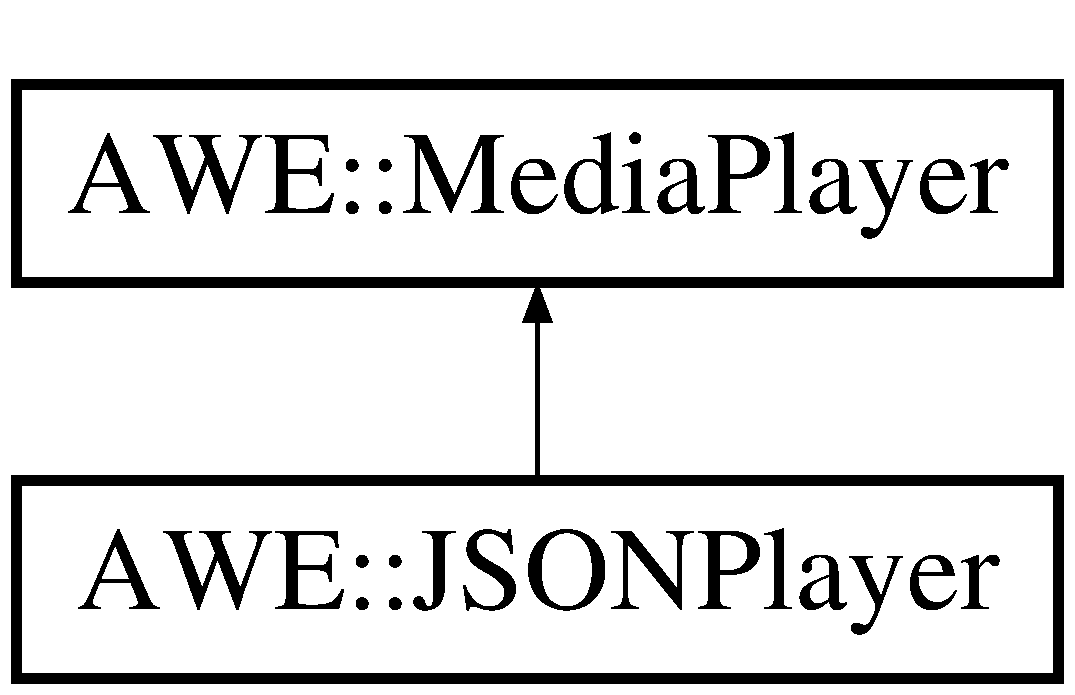
\includegraphics[height=2.000000cm]{class_a_w_e_1_1_j_s_o_n_player}
\end{center}
\end{figure}
\subsection*{Public Member Functions}
\begin{DoxyCompactItemize}
\item 
\hyperlink{class_a_w_e_1_1_j_s_o_n_player_a7aceda6a2e246528d952d4b50c0645e0}{J\-S\-O\-N\-Player} (\hyperlink{class_json_1_1_value}{Json\-::\-Value} \&player)
\begin{DoxyCompactList}\small\item\em Construct a media player from the given J\-S\-O\-N object. \end{DoxyCompactList}\item 
virtual int \hyperlink{class_a_w_e_1_1_j_s_o_n_player_a417957c7b0826ecef28b232a2cf9d49e}{play} (\hyperlink{class_a_w_e_1_1_media_file}{Media\-File} $\ast$file)
\begin{DoxyCompactList}\small\item\em Play the given file. \end{DoxyCompactList}\item 
virtual const std\-::string \& \hyperlink{class_a_w_e_1_1_j_s_o_n_player_a24bd164f654e3fda5587be04013bb366}{get\-Name} () const 
\begin{DoxyCompactList}\small\item\em Get the name of the player. \end{DoxyCompactList}\end{DoxyCompactItemize}


\subsection{Detailed Description}
Represents an external media player designed in a J\-S\-O\-N file. 

\subsection{Constructor \& Destructor Documentation}
\hypertarget{class_a_w_e_1_1_j_s_o_n_player_a7aceda6a2e246528d952d4b50c0645e0}{\index{A\-W\-E\-::\-J\-S\-O\-N\-Player@{A\-W\-E\-::\-J\-S\-O\-N\-Player}!J\-S\-O\-N\-Player@{J\-S\-O\-N\-Player}}
\index{J\-S\-O\-N\-Player@{J\-S\-O\-N\-Player}!AWE::JSONPlayer@{A\-W\-E\-::\-J\-S\-O\-N\-Player}}
\subsubsection[{J\-S\-O\-N\-Player}]{\setlength{\rightskip}{0pt plus 5cm}J\-S\-O\-N\-Player\-::\-J\-S\-O\-N\-Player (
\begin{DoxyParamCaption}
\item[{{\bf Json\-::\-Value} \&}]{player}
\end{DoxyParamCaption}
)}}\label{class_a_w_e_1_1_j_s_o_n_player_a7aceda6a2e246528d952d4b50c0645e0}


Construct a media player from the given J\-S\-O\-N object. 


\begin{DoxyParams}{Parameters}
{\em player} & The J\-S\-O\-N object representing this player. \\
\hline
\end{DoxyParams}


\subsection{Member Function Documentation}
\hypertarget{class_a_w_e_1_1_j_s_o_n_player_a24bd164f654e3fda5587be04013bb366}{\index{A\-W\-E\-::\-J\-S\-O\-N\-Player@{A\-W\-E\-::\-J\-S\-O\-N\-Player}!get\-Name@{get\-Name}}
\index{get\-Name@{get\-Name}!AWE::JSONPlayer@{A\-W\-E\-::\-J\-S\-O\-N\-Player}}
\subsubsection[{get\-Name}]{\setlength{\rightskip}{0pt plus 5cm}const string \& J\-S\-O\-N\-Player\-::get\-Name (
\begin{DoxyParamCaption}
{}
\end{DoxyParamCaption}
) const\hspace{0.3cm}{\ttfamily [virtual]}}}\label{class_a_w_e_1_1_j_s_o_n_player_a24bd164f654e3fda5587be04013bb366}


Get the name of the player. 

\begin{DoxyReturn}{Returns}
The name of the player. 
\end{DoxyReturn}


Implements \hyperlink{class_a_w_e_1_1_media_player_a59d47b0590a9cba607e2189947ea0239}{A\-W\-E\-::\-Media\-Player}.

\hypertarget{class_a_w_e_1_1_j_s_o_n_player_a417957c7b0826ecef28b232a2cf9d49e}{\index{A\-W\-E\-::\-J\-S\-O\-N\-Player@{A\-W\-E\-::\-J\-S\-O\-N\-Player}!play@{play}}
\index{play@{play}!AWE::JSONPlayer@{A\-W\-E\-::\-J\-S\-O\-N\-Player}}
\subsubsection[{play}]{\setlength{\rightskip}{0pt plus 5cm}int J\-S\-O\-N\-Player\-::play (
\begin{DoxyParamCaption}
\item[{{\bf Media\-File} $\ast$}]{file}
\end{DoxyParamCaption}
)\hspace{0.3cm}{\ttfamily [virtual]}}}\label{class_a_w_e_1_1_j_s_o_n_player_a417957c7b0826ecef28b232a2cf9d49e}


Play the given file. 


\begin{DoxyParams}{Parameters}
{\em file} & The media file to play.\\
\hline
\end{DoxyParams}
\begin{DoxyReturn}{Returns}
{\ttfamily true} if {\ttfamily file} played successfully, {\ttfamily false} otherwise. 
\end{DoxyReturn}


Implements \hyperlink{class_a_w_e_1_1_media_player_a8a7660cdf7306adf61a7c79831ee7171}{A\-W\-E\-::\-Media\-Player}.



The documentation for this class was generated from the following files\-:\begin{DoxyCompactItemize}
\item 
/\-Users/\-Alex/github/\-A\-W\-E\-Media\-Center/\-Code/player/A\-W\-E\-J\-S\-O\-N\-Player.\-h\item 
/\-Users/\-Alex/github/\-A\-W\-E\-Media\-Center/\-Code/player/A\-W\-E\-J\-S\-O\-N\-Player.\-cpp\end{DoxyCompactItemize}

\hypertarget{class_a_w_e_1_1_j_s_o_n_scraper}{\section{A\-W\-E\-:\-:J\-S\-O\-N\-Scraper Class Reference}
\label{class_a_w_e_1_1_j_s_o_n_scraper}\index{A\-W\-E\-::\-J\-S\-O\-N\-Scraper@{A\-W\-E\-::\-J\-S\-O\-N\-Scraper}}
}


A metadata scraper based on J\-S\-O\-N files.  




{\ttfamily \#include $<$A\-W\-E\-J\-S\-O\-N\-Scraper.\-h$>$}

Inheritance diagram for A\-W\-E\-:\-:J\-S\-O\-N\-Scraper\-:\begin{figure}[H]
\begin{center}
\leavevmode
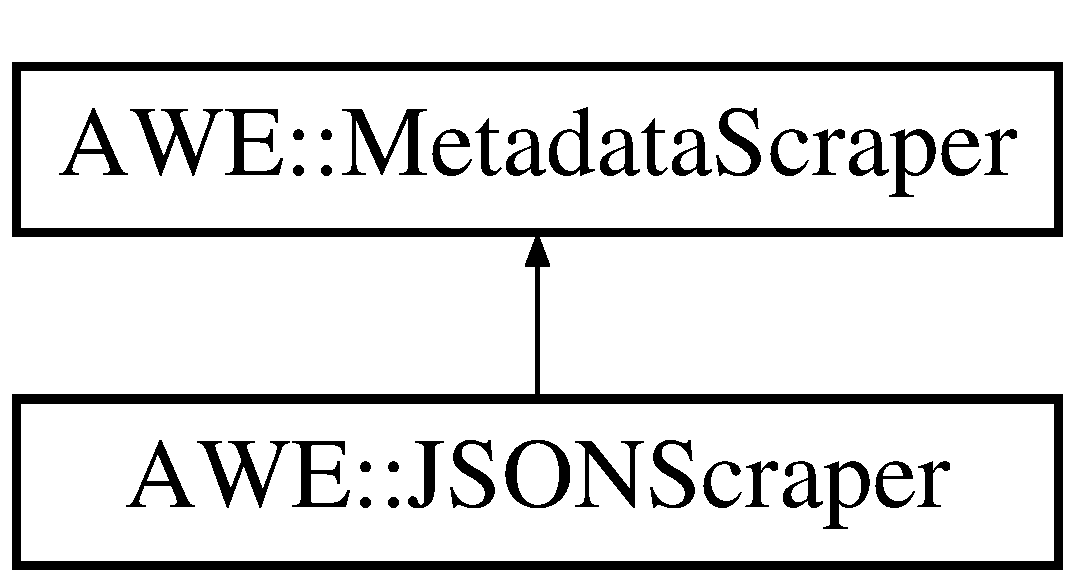
\includegraphics[height=2.000000cm]{class_a_w_e_1_1_j_s_o_n_scraper}
\end{center}
\end{figure}
\subsection*{Public Member Functions}
\begin{DoxyCompactItemize}
\item 
\hyperlink{class_a_w_e_1_1_j_s_o_n_scraper_ac6fe5d6f084e3b9ff5fdd1e5cd883351}{J\-S\-O\-N\-Scraper} (Q\-String name, Q\-String type)
\begin{DoxyCompactList}\small\item\em Construct a new J\-S\-O\-N-\/based scraper from the given name. \end{DoxyCompactList}\item 
virtual bool \hyperlink{class_a_w_e_1_1_j_s_o_n_scraper_a1b12fde072ef979911fcca4191c3c2a7}{prepare} (\hyperlink{class_a_w_e_1_1_global_settings}{Global\-Settings} $\ast$settings)
\begin{DoxyCompactList}\small\item\em Prepares the scraper by reading the scraper and type files. \end{DoxyCompactList}\item 
virtual bool \hyperlink{class_a_w_e_1_1_j_s_o_n_scraper_a883ec1b6814b4f192a28f32c8f47dd39}{scrape\-Data\-For\-File} (\hyperlink{class_a_w_e_1_1_media_item}{Media\-Item} $\ast$file, bool ask\-User, bool import, bool inherit\-Metadata)
\begin{DoxyCompactList}\small\item\em Retrieves metadata for a media file. \end{DoxyCompactList}\item 
virtual Q\-List$<$ \hyperlink{class_a_w_e_1_1_media_item}{Media\-Item} $\ast$ $>$ \hyperlink{class_a_w_e_1_1_j_s_o_n_scraper_a1ccab4a9c36f8420222a75de1282eb2f}{scrape\-Data\-For\-File} (\hyperlink{class_a_w_e_1_1_folder}{Folder} $\ast$place\-In\-Me, \hyperlink{class_a_w_e_1_1_global_settings}{Global\-Settings} $\ast$global\-Settings, Q\-Dir file, bool ask\-User, bool import, bool inherit\-Metadata)
\begin{DoxyCompactList}\small\item\em Create a media item (or multiple if applicable) from a given file or folder. \end{DoxyCompactList}\item 
virtual void \hyperlink{class_a_w_e_1_1_j_s_o_n_scraper_a0d1a05a4c7273ff1063518592d68501a}{deactivate} ()
\begin{DoxyCompactList}\small\item\em Destroys any used-\/up dynamic memory. \end{DoxyCompactList}\item 
virtual bool \hyperlink{class_a_w_e_1_1_j_s_o_n_scraper_abb4ca61ee617b473198a635c6f3ac57d}{is\-Valid} ()
\begin{DoxyCompactList}\small\item\em Determines if this is scraper can be used. \end{DoxyCompactList}\item 
virtual Q\-String \hyperlink{class_a_w_e_1_1_j_s_o_n_scraper_a9a2613e43da4d36040f704d0481fff50}{get\-Name} ()
\begin{DoxyCompactList}\small\item\em Gets the name of the scraper. \end{DoxyCompactList}\item 
virtual Q\-String \hyperlink{class_a_w_e_1_1_j_s_o_n_scraper_a95ff503c69c697cacc121182c4aa5ea4}{get\-Type} ()
\begin{DoxyCompactList}\small\item\em Gets the media type for this scraper. \end{DoxyCompactList}\end{DoxyCompactItemize}
\subsection*{Private Member Functions}
\begin{DoxyCompactItemize}
\item 
bool \hyperlink{class_a_w_e_1_1_j_s_o_n_scraper_aefc9dd0f99a2adab9b595ef3b3582c8b}{execute\-Procedure} (\hyperlink{class_json_1_1_value}{Json\-::\-Value} \&procedure, Q\-Regular\-Expression\-Match backrefs, bool ask\-User, bool import, bool inherit\-Metadata)
\begin{DoxyCompactList}\small\item\em Execute a specific procedure from a {\ttfamily \char`\"{}procedures\char`\"{}} array. \end{DoxyCompactList}\item 
bool \hyperlink{class_a_w_e_1_1_j_s_o_n_scraper_a575f13fe24c45ea6a06d61569ed22fe7}{use\-Match\-For\-Procedure} (\hyperlink{class_json_1_1_value}{Json\-::\-Value} \&procedure, Q\-Regular\-Expression\-Match backrefs, bool ask\-User, bool import, bool inherit\-Metadata)
\begin{DoxyCompactList}\small\item\em Helper function that sets properties and executes sub-\/procedures. \end{DoxyCompactList}\item 
void \hyperlink{class_a_w_e_1_1_j_s_o_n_scraper_a339670a46a5b55b1c59b3ddba5986742}{import\-Files} (\hyperlink{class_json_1_1_value}{Json\-::\-Value} \&props)
\begin{DoxyCompactList}\small\item\em Helper function that imports the files in the given {\ttfamily \hyperlink{class_json_1_1_value}{Json\-::\-Value}}. \end{DoxyCompactList}\item 
int \hyperlink{class_a_w_e_1_1_j_s_o_n_scraper_afb2118a214f52055259d4e214c147cf9}{replace\-Backrefs} (Q\-String \&pseudo\-\_\-reg, Q\-Regular\-Expression\-Match backrefs)
\begin{DoxyCompactList}\small\item\em Replace the backreferences in {\ttfamily pseudo\-\_\-reg} with the references from {\ttfamily backrefs}. \end{DoxyCompactList}\item 
Q\-String \& \hyperlink{class_a_w_e_1_1_j_s_o_n_scraper_a406666e30d724336826cdaae6ede7c8c}{get\-File\-Contents} (Q\-String file)
\begin{DoxyCompactList}\small\item\em Get the contents of a file, either from the already opened files or a new file. \end{DoxyCompactList}\item 
bool \hyperlink{class_a_w_e_1_1_j_s_o_n_scraper_ac83bcfb3d69108024c23ff49e8b8c274}{check\-Validity} ()
\begin{DoxyCompactList}\small\item\em Does a test run of the procedures to decide if this scraper is valid. \end{DoxyCompactList}\item 
bool \hyperlink{class_a_w_e_1_1_j_s_o_n_scraper_ac73167b683a6dec42cd84211e337dc46}{check\-Procedure\-Validity} (\hyperlink{class_json_1_1_value}{Json\-::\-Value} \&procedure, int cap\-Count)
\begin{DoxyCompactList}\small\item\em Does a test run of a procedure to decide if it is valid. \end{DoxyCompactList}\end{DoxyCompactItemize}
\subsection*{Private Attributes}
\begin{DoxyCompactItemize}
\item 
\hypertarget{class_a_w_e_1_1_j_s_o_n_scraper_a5ca0c55dde4c469a4a09680257792d9d}{bool \hyperlink{class_a_w_e_1_1_j_s_o_n_scraper_a5ca0c55dde4c469a4a09680257792d9d}{my\-Validity}}\label{class_a_w_e_1_1_j_s_o_n_scraper_a5ca0c55dde4c469a4a09680257792d9d}

\begin{DoxyCompactList}\small\item\em Can this be used effectively? \end{DoxyCompactList}\item 
\hypertarget{class_a_w_e_1_1_j_s_o_n_scraper_a0073f1a2fbbc412756c6ae2318972d39}{Q\-String \hyperlink{class_a_w_e_1_1_j_s_o_n_scraper_a0073f1a2fbbc412756c6ae2318972d39}{my\-Name}}\label{class_a_w_e_1_1_j_s_o_n_scraper_a0073f1a2fbbc412756c6ae2318972d39}

\begin{DoxyCompactList}\small\item\em Name of the scraper. \end{DoxyCompactList}\item 
\hypertarget{class_a_w_e_1_1_j_s_o_n_scraper_a53b36c31016a1c503630c41b1d5b7901}{Q\-String \hyperlink{class_a_w_e_1_1_j_s_o_n_scraper_a53b36c31016a1c503630c41b1d5b7901}{my\-Type}}\label{class_a_w_e_1_1_j_s_o_n_scraper_a53b36c31016a1c503630c41b1d5b7901}

\begin{DoxyCompactList}\small\item\em The type of the scraper. \end{DoxyCompactList}\item 
\hypertarget{class_a_w_e_1_1_j_s_o_n_scraper_a1a569b18d21b70f8777fe24605860efb}{\hyperlink{class_json_1_1_value}{Json\-::\-Value} \hyperlink{class_a_w_e_1_1_j_s_o_n_scraper_a1a569b18d21b70f8777fe24605860efb}{my\-Scraper}}\label{class_a_w_e_1_1_j_s_o_n_scraper_a1a569b18d21b70f8777fe24605860efb}

\begin{DoxyCompactList}\small\item\em The data determining how to scrape. \end{DoxyCompactList}\item 
\hypertarget{class_a_w_e_1_1_j_s_o_n_scraper_a72e4f32c2432abd2f3e9259d1227cb5a}{\hyperlink{class_json_1_1_value}{Json\-::\-Value} \hyperlink{class_a_w_e_1_1_j_s_o_n_scraper_a72e4f32c2432abd2f3e9259d1227cb5a}{my\-Default\-Properties}}\label{class_a_w_e_1_1_j_s_o_n_scraper_a72e4f32c2432abd2f3e9259d1227cb5a}

\begin{DoxyCompactList}\small\item\em The global settings. \end{DoxyCompactList}\item 
\hypertarget{class_a_w_e_1_1_j_s_o_n_scraper_a9672341060610ef66334d232f1319149}{\hyperlink{class_a_w_e_1_1_media_item}{Media\-Item} $\ast$ \hyperlink{class_a_w_e_1_1_j_s_o_n_scraper_a9672341060610ef66334d232f1319149}{my\-Current\-File}}\label{class_a_w_e_1_1_j_s_o_n_scraper_a9672341060610ef66334d232f1319149}

\begin{DoxyCompactList}\small\item\em The current file. \end{DoxyCompactList}\item 
\hypertarget{class_a_w_e_1_1_j_s_o_n_scraper_a00f08f99c83dbeadd7fdf44d6677ff47}{\hyperlink{class_a_w_e_1_1_folder}{Folder} $\ast$ \hyperlink{class_a_w_e_1_1_j_s_o_n_scraper_a00f08f99c83dbeadd7fdf44d6677ff47}{my\-Current\-Folder}}\label{class_a_w_e_1_1_j_s_o_n_scraper_a00f08f99c83dbeadd7fdf44d6677ff47}

\begin{DoxyCompactList}\small\item\em The folder contianing my\-Current\-File. \end{DoxyCompactList}\item 
\hypertarget{class_a_w_e_1_1_j_s_o_n_scraper_a91f5819597613553161fe9bf22581c31}{\hyperlink{class_a_w_e_1_1_global_settings}{Global\-Settings} $\ast$ \hyperlink{class_a_w_e_1_1_j_s_o_n_scraper_a91f5819597613553161fe9bf22581c31}{my\-Global\-Settings}}\label{class_a_w_e_1_1_j_s_o_n_scraper_a91f5819597613553161fe9bf22581c31}

\begin{DoxyCompactList}\small\item\em The global settings of \hyperlink{class_a_w_e_1_1_a_w_e_m_c}{A\-W\-E\-M\-C}. \end{DoxyCompactList}\item 
\hypertarget{class_a_w_e_1_1_j_s_o_n_scraper_a17088ef91b31db71172616f62b2d257c}{Q\-Hash$<$ Q\-String, Q\-String $>$ \hyperlink{class_a_w_e_1_1_j_s_o_n_scraper_a17088ef91b31db71172616f62b2d257c}{my\-Metadata\-Files}}\label{class_a_w_e_1_1_j_s_o_n_scraper_a17088ef91b31db71172616f62b2d257c}

\begin{DoxyCompactList}\small\item\em Maps file onto file contents (for speed boost). \end{DoxyCompactList}\item 
\hypertarget{class_a_w_e_1_1_j_s_o_n_scraper_ade471d4c08caf575269396b9321278ab}{Q\-Hash$<$ Q\-String, Q\-String $>$ \hyperlink{class_a_w_e_1_1_j_s_o_n_scraper_ade471d4c08caf575269396b9321278ab}{my\-Inherited\-Properties}}\label{class_a_w_e_1_1_j_s_o_n_scraper_ade471d4c08caf575269396b9321278ab}

\begin{DoxyCompactList}\small\item\em Maps {\ttfamily my\-Current\-File} props onto {\ttfamily my\-Current\-Folder} props. \end{DoxyCompactList}\item 
\hypertarget{class_a_w_e_1_1_j_s_o_n_scraper_af8181e179af7036bee14fa3f04651c99}{Q\-Set$<$ Q\-String $>$ \hyperlink{class_a_w_e_1_1_j_s_o_n_scraper_af8181e179af7036bee14fa3f04651c99}{my\-File\-Properties}}\label{class_a_w_e_1_1_j_s_o_n_scraper_af8181e179af7036bee14fa3f04651c99}

\begin{DoxyCompactList}\small\item\em Set of file properties. \end{DoxyCompactList}\end{DoxyCompactItemize}


\subsection{Detailed Description}
A metadata scraper based on J\-S\-O\-N files. 

\begin{DoxyRefDesc}{Todo}
\item[\hyperlink{todo__todo000002}{Todo}]Change {\ttfamily my\-Type} to be the mystical know-\/all configuration object.\end{DoxyRefDesc}


One way of defining a scraper is through a J\-S\-O\-N file interpreted by an instantiation of this class. To read more about the format of such a J\-S\-O\-N file, read this document.

For information on media types, read ../type/\-R\-E\-A\-D\-M\-E.md \char`\"{}this document\char`\"{}. 

\subsection{Constructor \& Destructor Documentation}
\hypertarget{class_a_w_e_1_1_j_s_o_n_scraper_ac6fe5d6f084e3b9ff5fdd1e5cd883351}{\index{A\-W\-E\-::\-J\-S\-O\-N\-Scraper@{A\-W\-E\-::\-J\-S\-O\-N\-Scraper}!J\-S\-O\-N\-Scraper@{J\-S\-O\-N\-Scraper}}
\index{J\-S\-O\-N\-Scraper@{J\-S\-O\-N\-Scraper}!AWE::JSONScraper@{A\-W\-E\-::\-J\-S\-O\-N\-Scraper}}
\subsubsection[{J\-S\-O\-N\-Scraper}]{\setlength{\rightskip}{0pt plus 5cm}J\-S\-O\-N\-Scraper\-::\-J\-S\-O\-N\-Scraper (
\begin{DoxyParamCaption}
\item[{Q\-String}]{name, }
\item[{Q\-String}]{type}
\end{DoxyParamCaption}
)}}\label{class_a_w_e_1_1_j_s_o_n_scraper_ac6fe5d6f084e3b9ff5fdd1e5cd883351}


Construct a new J\-S\-O\-N-\/based scraper from the given name. 


\begin{DoxyParams}[1]{Parameters}
\mbox{\tt in}  & {\em name} & The name of the scraper. \\
\hline
\mbox{\tt in}  & {\em type} & The media type for this scraper. \\
\hline
\end{DoxyParams}


\subsection{Member Function Documentation}
\hypertarget{class_a_w_e_1_1_j_s_o_n_scraper_ac73167b683a6dec42cd84211e337dc46}{\index{A\-W\-E\-::\-J\-S\-O\-N\-Scraper@{A\-W\-E\-::\-J\-S\-O\-N\-Scraper}!check\-Procedure\-Validity@{check\-Procedure\-Validity}}
\index{check\-Procedure\-Validity@{check\-Procedure\-Validity}!AWE::JSONScraper@{A\-W\-E\-::\-J\-S\-O\-N\-Scraper}}
\subsubsection[{check\-Procedure\-Validity}]{\setlength{\rightskip}{0pt plus 5cm}bool J\-S\-O\-N\-Scraper\-::check\-Procedure\-Validity (
\begin{DoxyParamCaption}
\item[{{\bf Json\-::\-Value} \&}]{procedure, }
\item[{int}]{cap\-Count}
\end{DoxyParamCaption}
)\hspace{0.3cm}{\ttfamily [private]}}}\label{class_a_w_e_1_1_j_s_o_n_scraper_ac73167b683a6dec42cd84211e337dc46}


Does a test run of a procedure to decide if it is valid. 

\begin{DoxyRefDesc}{Todo}
\item[\hyperlink{todo__todo000006}{Todo}]This entire function (which at the moment just returns {\ttfamily true})\end{DoxyRefDesc}



\begin{DoxyParams}[1]{Parameters}
\mbox{\tt in}  & {\em procedure} & The procedure to check. \\
\hline
\mbox{\tt in}  & {\em cap\-Count} & The number of backrefs passed to the procedure.\\
\hline
\end{DoxyParams}
\begin{DoxyReturn}{Returns}
{\ttfamily true} if {\ttfamily procedure} is safe to use, {\ttfamily false} otherwise. 
\end{DoxyReturn}
\hypertarget{class_a_w_e_1_1_j_s_o_n_scraper_ac83bcfb3d69108024c23ff49e8b8c274}{\index{A\-W\-E\-::\-J\-S\-O\-N\-Scraper@{A\-W\-E\-::\-J\-S\-O\-N\-Scraper}!check\-Validity@{check\-Validity}}
\index{check\-Validity@{check\-Validity}!AWE::JSONScraper@{A\-W\-E\-::\-J\-S\-O\-N\-Scraper}}
\subsubsection[{check\-Validity}]{\setlength{\rightskip}{0pt plus 5cm}bool J\-S\-O\-N\-Scraper\-::check\-Validity (
\begin{DoxyParamCaption}
{}
\end{DoxyParamCaption}
)\hspace{0.3cm}{\ttfamily [private]}}}\label{class_a_w_e_1_1_j_s_o_n_scraper_ac83bcfb3d69108024c23ff49e8b8c274}


Does a test run of the procedures to decide if this scraper is valid. 

\begin{DoxyRefDesc}{Todo}
\item[\hyperlink{todo__todo000005}{Todo}]This entire function (which at the moment just returns {\ttfamily true})\end{DoxyRefDesc}


\begin{DoxyReturn}{Returns}
{\ttfamily true} if this scraper is safe to use, {\ttfamily false} otherwise. 
\end{DoxyReturn}
\hypertarget{class_a_w_e_1_1_j_s_o_n_scraper_a0d1a05a4c7273ff1063518592d68501a}{\index{A\-W\-E\-::\-J\-S\-O\-N\-Scraper@{A\-W\-E\-::\-J\-S\-O\-N\-Scraper}!deactivate@{deactivate}}
\index{deactivate@{deactivate}!AWE::JSONScraper@{A\-W\-E\-::\-J\-S\-O\-N\-Scraper}}
\subsubsection[{deactivate}]{\setlength{\rightskip}{0pt plus 5cm}void J\-S\-O\-N\-Scraper\-::deactivate (
\begin{DoxyParamCaption}
{}
\end{DoxyParamCaption}
)\hspace{0.3cm}{\ttfamily [virtual]}}}\label{class_a_w_e_1_1_j_s_o_n_scraper_a0d1a05a4c7273ff1063518592d68501a}


Destroys any used-\/up dynamic memory. 

This helps with memory management. 

Implements \hyperlink{class_a_w_e_1_1_metadata_scraper_a9a90e9974be775dff73c004ada209cb0}{A\-W\-E\-::\-Metadata\-Scraper}.

\hypertarget{class_a_w_e_1_1_j_s_o_n_scraper_aefc9dd0f99a2adab9b595ef3b3582c8b}{\index{A\-W\-E\-::\-J\-S\-O\-N\-Scraper@{A\-W\-E\-::\-J\-S\-O\-N\-Scraper}!execute\-Procedure@{execute\-Procedure}}
\index{execute\-Procedure@{execute\-Procedure}!AWE::JSONScraper@{A\-W\-E\-::\-J\-S\-O\-N\-Scraper}}
\subsubsection[{execute\-Procedure}]{\setlength{\rightskip}{0pt plus 5cm}bool J\-S\-O\-N\-Scraper\-::execute\-Procedure (
\begin{DoxyParamCaption}
\item[{{\bf Json\-::\-Value} \&}]{procedure, }
\item[{Q\-Regular\-Expression\-Match}]{backrefs, }
\item[{bool}]{ask\-User, }
\item[{bool}]{import, }
\item[{bool}]{inherit\-Metadata}
\end{DoxyParamCaption}
)\hspace{0.3cm}{\ttfamily [private]}}}\label{class_a_w_e_1_1_j_s_o_n_scraper_aefc9dd0f99a2adab9b595ef3b3582c8b}


Execute a specific procedure from a {\ttfamily \char`\"{}procedures\char`\"{}} array. 


\begin{DoxyParams}[1]{Parameters}
\mbox{\tt in}  & {\em procedure} & The procedure to execute. \\
\hline
\mbox{\tt in}  & {\em backrefs} & The backreferences to use on the {\ttfamily \char`\"{}look in file\char`\"{}} and {\ttfamily \char`\"{}for\char`\"{}} tags. \\
\hline
\mbox{\tt in}  & {\em ask\-User} & {\ttfamily true} if the user wants semi-\/automatic scraping, {\ttfamily false} if completely automatic. \\
\hline
\mbox{\tt in}  & {\em import} & {\ttfamily true} if the user wants to import files, {\ttfamily false} if the user wants links. \\
\hline
\mbox{\tt in}  & {\em inherit\-Metadata} & {\ttfamily true} if designated metadata items should be inherited from the containing folder, {\ttfamily false} otherwise.\\
\hline
\end{DoxyParams}
\begin{DoxyReturn}{Returns}
{\ttfamily true} if the procedure ran without issue, {\ttfamily false} otherwise. 
\end{DoxyReturn}
\hypertarget{class_a_w_e_1_1_j_s_o_n_scraper_a406666e30d724336826cdaae6ede7c8c}{\index{A\-W\-E\-::\-J\-S\-O\-N\-Scraper@{A\-W\-E\-::\-J\-S\-O\-N\-Scraper}!get\-File\-Contents@{get\-File\-Contents}}
\index{get\-File\-Contents@{get\-File\-Contents}!AWE::JSONScraper@{A\-W\-E\-::\-J\-S\-O\-N\-Scraper}}
\subsubsection[{get\-File\-Contents}]{\setlength{\rightskip}{0pt plus 5cm}Q\-String \& J\-S\-O\-N\-Scraper\-::get\-File\-Contents (
\begin{DoxyParamCaption}
\item[{Q\-String}]{file}
\end{DoxyParamCaption}
)\hspace{0.3cm}{\ttfamily [private]}}}\label{class_a_w_e_1_1_j_s_o_n_scraper_a406666e30d724336826cdaae6ede7c8c}


Get the contents of a file, either from the already opened files or a new file. 


\begin{DoxyParams}[1]{Parameters}
\mbox{\tt in}  & {\em file} & The file to get the contents for.\\
\hline
\end{DoxyParams}
\begin{DoxyReturn}{Returns}
The contents of {\ttfamily file}. 
\end{DoxyReturn}
\hypertarget{class_a_w_e_1_1_j_s_o_n_scraper_a9a2613e43da4d36040f704d0481fff50}{\index{A\-W\-E\-::\-J\-S\-O\-N\-Scraper@{A\-W\-E\-::\-J\-S\-O\-N\-Scraper}!get\-Name@{get\-Name}}
\index{get\-Name@{get\-Name}!AWE::JSONScraper@{A\-W\-E\-::\-J\-S\-O\-N\-Scraper}}
\subsubsection[{get\-Name}]{\setlength{\rightskip}{0pt plus 5cm}Q\-String J\-S\-O\-N\-Scraper\-::get\-Name (
\begin{DoxyParamCaption}
{}
\end{DoxyParamCaption}
)\hspace{0.3cm}{\ttfamily [virtual]}}}\label{class_a_w_e_1_1_j_s_o_n_scraper_a9a2613e43da4d36040f704d0481fff50}


Gets the name of the scraper. 

\begin{DoxyReturn}{Returns}
The name of the scraper. 
\end{DoxyReturn}


Implements \hyperlink{class_a_w_e_1_1_metadata_scraper_ace0871b6861e04ec3ff39cba70606d29}{A\-W\-E\-::\-Metadata\-Scraper}.

\hypertarget{class_a_w_e_1_1_j_s_o_n_scraper_a95ff503c69c697cacc121182c4aa5ea4}{\index{A\-W\-E\-::\-J\-S\-O\-N\-Scraper@{A\-W\-E\-::\-J\-S\-O\-N\-Scraper}!get\-Type@{get\-Type}}
\index{get\-Type@{get\-Type}!AWE::JSONScraper@{A\-W\-E\-::\-J\-S\-O\-N\-Scraper}}
\subsubsection[{get\-Type}]{\setlength{\rightskip}{0pt plus 5cm}Q\-String J\-S\-O\-N\-Scraper\-::get\-Type (
\begin{DoxyParamCaption}
{}
\end{DoxyParamCaption}
)\hspace{0.3cm}{\ttfamily [virtual]}}}\label{class_a_w_e_1_1_j_s_o_n_scraper_a95ff503c69c697cacc121182c4aa5ea4}


Gets the media type for this scraper. 

\begin{DoxyReturn}{Returns}
The media type name for the scraper. 
\end{DoxyReturn}


Implements \hyperlink{class_a_w_e_1_1_metadata_scraper_a71f1b614a3196d5d8b68e3d216896e3d}{A\-W\-E\-::\-Metadata\-Scraper}.

\hypertarget{class_a_w_e_1_1_j_s_o_n_scraper_a339670a46a5b55b1c59b3ddba5986742}{\index{A\-W\-E\-::\-J\-S\-O\-N\-Scraper@{A\-W\-E\-::\-J\-S\-O\-N\-Scraper}!import\-Files@{import\-Files}}
\index{import\-Files@{import\-Files}!AWE::JSONScraper@{A\-W\-E\-::\-J\-S\-O\-N\-Scraper}}
\subsubsection[{import\-Files}]{\setlength{\rightskip}{0pt plus 5cm}void J\-S\-O\-N\-Scraper\-::import\-Files (
\begin{DoxyParamCaption}
\item[{{\bf Json\-::\-Value} \&}]{props}
\end{DoxyParamCaption}
)\hspace{0.3cm}{\ttfamily [private]}}}\label{class_a_w_e_1_1_j_s_o_n_scraper_a339670a46a5b55b1c59b3ddba5986742}


Helper function that imports the files in the given {\ttfamily \hyperlink{class_json_1_1_value}{Json\-::\-Value}}. 

This is used for the {\ttfamily \char`\"{}force copy\char`\"{}} and {\ttfamily \char`\"{}copy\char`\"{}} tags.


\begin{DoxyParams}[1]{Parameters}
\mbox{\tt in}  & {\em props} & The properties that contain files to import. \\
\hline
\end{DoxyParams}
\hypertarget{class_a_w_e_1_1_j_s_o_n_scraper_abb4ca61ee617b473198a635c6f3ac57d}{\index{A\-W\-E\-::\-J\-S\-O\-N\-Scraper@{A\-W\-E\-::\-J\-S\-O\-N\-Scraper}!is\-Valid@{is\-Valid}}
\index{is\-Valid@{is\-Valid}!AWE::JSONScraper@{A\-W\-E\-::\-J\-S\-O\-N\-Scraper}}
\subsubsection[{is\-Valid}]{\setlength{\rightskip}{0pt plus 5cm}bool J\-S\-O\-N\-Scraper\-::is\-Valid (
\begin{DoxyParamCaption}
{}
\end{DoxyParamCaption}
)\hspace{0.3cm}{\ttfamily [virtual]}}}\label{class_a_w_e_1_1_j_s_o_n_scraper_abb4ca61ee617b473198a635c6f3ac57d}


Determines if this is scraper can be used. 

\begin{DoxyReturn}{Returns}
{\ttfamily true} if this scraper can be used successfully, {\ttfamily false} otherwise. 
\end{DoxyReturn}


Implements \hyperlink{class_a_w_e_1_1_metadata_scraper_a06f9da8e43ac52378ec15fc849e42eb8}{A\-W\-E\-::\-Metadata\-Scraper}.

\hypertarget{class_a_w_e_1_1_j_s_o_n_scraper_a1b12fde072ef979911fcca4191c3c2a7}{\index{A\-W\-E\-::\-J\-S\-O\-N\-Scraper@{A\-W\-E\-::\-J\-S\-O\-N\-Scraper}!prepare@{prepare}}
\index{prepare@{prepare}!AWE::JSONScraper@{A\-W\-E\-::\-J\-S\-O\-N\-Scraper}}
\subsubsection[{prepare}]{\setlength{\rightskip}{0pt plus 5cm}bool J\-S\-O\-N\-Scraper\-::prepare (
\begin{DoxyParamCaption}
\item[{{\bf Global\-Settings} $\ast$}]{settings}
\end{DoxyParamCaption}
)\hspace{0.3cm}{\ttfamily [virtual]}}}\label{class_a_w_e_1_1_j_s_o_n_scraper_a1b12fde072ef979911fcca4191c3c2a7}


Prepares the scraper by reading the scraper and type files. 

This helps with memory management.


\begin{DoxyParams}[1]{Parameters}
\mbox{\tt in}  & {\em settings} & The ../settings/\-R\-E\-A\-D\-M\-E.md \char`\"{}global settings of A\-W\-E\-M\-C\char`\"{}.\\
\hline
\end{DoxyParams}
\begin{DoxyReturn}{Returns}
{\ttfamily true} if the scraper was able to prepare itself, {\ttfamily false} if an error occured and scraping should be aborted. Generally, a {\ttfamily false} result here means that the J\-S\-O\-N file was incorrectly written. 
\end{DoxyReturn}


Implements \hyperlink{class_a_w_e_1_1_metadata_scraper_a92f9039770add633140b825bf41bc30a}{A\-W\-E\-::\-Metadata\-Scraper}.

\hypertarget{class_a_w_e_1_1_j_s_o_n_scraper_afb2118a214f52055259d4e214c147cf9}{\index{A\-W\-E\-::\-J\-S\-O\-N\-Scraper@{A\-W\-E\-::\-J\-S\-O\-N\-Scraper}!replace\-Backrefs@{replace\-Backrefs}}
\index{replace\-Backrefs@{replace\-Backrefs}!AWE::JSONScraper@{A\-W\-E\-::\-J\-S\-O\-N\-Scraper}}
\subsubsection[{replace\-Backrefs}]{\setlength{\rightskip}{0pt plus 5cm}int J\-S\-O\-N\-Scraper\-::replace\-Backrefs (
\begin{DoxyParamCaption}
\item[{Q\-String \&}]{pseudo\-\_\-reg, }
\item[{Q\-Regular\-Expression\-Match}]{backrefs}
\end{DoxyParamCaption}
)\hspace{0.3cm}{\ttfamily [private]}}}\label{class_a_w_e_1_1_j_s_o_n_scraper_afb2118a214f52055259d4e214c147cf9}


Replace the backreferences in {\ttfamily pseudo\-\_\-reg} with the references from {\ttfamily backrefs}. 

{\ttfamily pseudo\-\_\-reg} should be formatted according to \href{http://www.cplusplus.com/reference/regex/match_replace/}{\tt this function's} {\ttfamily fmt} parameter.


\begin{DoxyParams}[1]{Parameters}
\mbox{\tt out}  & {\em pseudo\-\_\-reg} & The {\ttfamily Q\-String} with the references to replace. \\
\hline
\mbox{\tt in}  & {\em backrefs} & The backreferences to use.\\
\hline
\end{DoxyParams}
\begin{DoxyReturn}{Returns}
The highest backref requested. 
\end{DoxyReturn}
\hypertarget{class_a_w_e_1_1_j_s_o_n_scraper_a883ec1b6814b4f192a28f32c8f47dd39}{\index{A\-W\-E\-::\-J\-S\-O\-N\-Scraper@{A\-W\-E\-::\-J\-S\-O\-N\-Scraper}!scrape\-Data\-For\-File@{scrape\-Data\-For\-File}}
\index{scrape\-Data\-For\-File@{scrape\-Data\-For\-File}!AWE::JSONScraper@{A\-W\-E\-::\-J\-S\-O\-N\-Scraper}}
\subsubsection[{scrape\-Data\-For\-File}]{\setlength{\rightskip}{0pt plus 5cm}bool J\-S\-O\-N\-Scraper\-::scrape\-Data\-For\-File (
\begin{DoxyParamCaption}
\item[{{\bf Media\-Item} $\ast$}]{file, }
\item[{bool}]{ask\-User, }
\item[{bool}]{import, }
\item[{bool}]{inherit\-Metadata}
\end{DoxyParamCaption}
)\hspace{0.3cm}{\ttfamily [virtual]}}}\label{class_a_w_e_1_1_j_s_o_n_scraper_a883ec1b6814b4f192a28f32c8f47dd39}


Retrieves metadata for a media file. 

To construct your J\-S\-O\-N file, you should use \href{http://jsoncpp.sourceforge.net}{\tt jsoncpp}.

{\ttfamily ask\-User} tells your scraper if the user wants to be given a list of choices for certain things. You should N\-O\-T ask the user for everything if {\ttfamily ask\-User} is true; only basic things like, \char`\"{}\-Which icon do you want to use?\char`\"{}

{\ttfamily import} specifies if the files you get should be copied into \hyperlink{class_a_w_e_1_1_a_w_e_m_c}{A\-W\-E\-M\-C}'s folders. Do N\-O\-T copy the media file.

\begin{DoxyRefDesc}{Todo}
\item[\hyperlink{todo__todo000003}{Todo}]boolean flags\end{DoxyRefDesc}



\begin{DoxyParams}[1]{Parameters}
\mbox{\tt in,out}  & {\em file} & The media file to get metadata for. \\
\hline
\mbox{\tt in}  & {\em ask\-User} & {\ttfamily true} if the user wants to be given choices, {\ttfamily false} otherwise. \\
\hline
\mbox{\tt in}  & {\em import} & {\ttfamily true} if the user wants to import metadata files, {\ttfamily false} otherwise. \\
\hline
\mbox{\tt in}  & {\em inherit\-Metadata} & {\ttfamily true} if designated metadata items should be inherited from the containing folder, {\ttfamily false} otherwise.\\
\hline
\end{DoxyParams}
\begin{DoxyReturn}{Returns}
{\ttfamily true} if the scraper was able to get the metadata, {\ttfamily false} if it was not. 
\end{DoxyReturn}


Implements \hyperlink{class_a_w_e_1_1_metadata_scraper_a14f10736d12ada980b4c64a906ebe9a6}{A\-W\-E\-::\-Metadata\-Scraper}.

\hypertarget{class_a_w_e_1_1_j_s_o_n_scraper_a1ccab4a9c36f8420222a75de1282eb2f}{\index{A\-W\-E\-::\-J\-S\-O\-N\-Scraper@{A\-W\-E\-::\-J\-S\-O\-N\-Scraper}!scrape\-Data\-For\-File@{scrape\-Data\-For\-File}}
\index{scrape\-Data\-For\-File@{scrape\-Data\-For\-File}!AWE::JSONScraper@{A\-W\-E\-::\-J\-S\-O\-N\-Scraper}}
\subsubsection[{scrape\-Data\-For\-File}]{\setlength{\rightskip}{0pt plus 5cm}Q\-List$<$ {\bf Media\-Item} $\ast$ $>$ J\-S\-O\-N\-Scraper\-::scrape\-Data\-For\-File (
\begin{DoxyParamCaption}
\item[{{\bf Folder} $\ast$}]{place\-In\-Me, }
\item[{{\bf Global\-Settings} $\ast$}]{global\-Settings, }
\item[{Q\-Dir}]{file, }
\item[{bool}]{ask\-User, }
\item[{bool}]{import, }
\item[{bool}]{inherit\-Metadata}
\end{DoxyParamCaption}
)\hspace{0.3cm}{\ttfamily [virtual]}}}\label{class_a_w_e_1_1_j_s_o_n_scraper_a1ccab4a9c36f8420222a75de1282eb2f}


Create a media item (or multiple if applicable) from a given file or folder. 

To construct your J\-S\-O\-N file, you should use \href{http://jsoncpp.sourceforge.net}{\tt Json\-Cpp}.

{\ttfamily ask\-User} tells your scraper if the user wants to be given a list of choices for certain things. You should N\-O\-T ask the user for everything if {\ttfamily ask\-User} is true; only basic things like, \char`\"{}\-Which icon do you want to use?\char`\"{}

{\ttfamily import} specifies if the files you get should be copied into \hyperlink{class_a_w_e_1_1_a_w_e_m_c}{A\-W\-E\-M\-C}'s folders. Do N\-O\-T copy the media file.

{\ttfamily inherit\-Metadata} determines if data that could be inherited from the folder should be.

\begin{DoxyRefDesc}{Todo}
\item[\hyperlink{todo__todo000004}{Todo}]boolean flags\end{DoxyRefDesc}



\begin{DoxyParams}[1]{Parameters}
\mbox{\tt out}  & {\em place\-In\-Me} & The {\ttfamily \hyperlink{class_a_w_e_1_1_folder}{Folder}} to put the created items in. \\
\hline
\mbox{\tt in}  & {\em file} & The file or folder to get media items for. \\
\hline
\mbox{\tt in}  & {\em global\-Settings} & The global settings of \hyperlink{class_a_w_e_1_1_a_w_e_m_c}{A\-W\-E\-M\-C}. \\
\hline
\mbox{\tt in}  & {\em ask\-User} & {\ttfamily true} if the user wants to be given choices, {\ttfamily false} otherwise. \\
\hline
\mbox{\tt in}  & {\em import} & {\ttfamily true} if the user wants to import metadata files, {\ttfamily false} otherwise. \\
\hline
\mbox{\tt in}  & {\em inherit\-Metadata} & {\ttfamily true} if designated metadata items should be inherited from the containing folder, {\ttfamily false} otherwise.\\
\hline
\end{DoxyParams}
\begin{DoxyReturn}{Returns}
A list of media items for the given file. The list is empty if the file does not match. 
\end{DoxyReturn}


Implements \hyperlink{class_a_w_e_1_1_metadata_scraper_af3708cc05181299d7c5b37afc1568b3d}{A\-W\-E\-::\-Metadata\-Scraper}.

\hypertarget{class_a_w_e_1_1_j_s_o_n_scraper_a575f13fe24c45ea6a06d61569ed22fe7}{\index{A\-W\-E\-::\-J\-S\-O\-N\-Scraper@{A\-W\-E\-::\-J\-S\-O\-N\-Scraper}!use\-Match\-For\-Procedure@{use\-Match\-For\-Procedure}}
\index{use\-Match\-For\-Procedure@{use\-Match\-For\-Procedure}!AWE::JSONScraper@{A\-W\-E\-::\-J\-S\-O\-N\-Scraper}}
\subsubsection[{use\-Match\-For\-Procedure}]{\setlength{\rightskip}{0pt plus 5cm}bool J\-S\-O\-N\-Scraper\-::use\-Match\-For\-Procedure (
\begin{DoxyParamCaption}
\item[{{\bf Json\-::\-Value} \&}]{procedure, }
\item[{Q\-Regular\-Expression\-Match}]{backrefs, }
\item[{bool}]{ask\-User, }
\item[{bool}]{import, }
\item[{bool}]{inherit\-Metadata}
\end{DoxyParamCaption}
)\hspace{0.3cm}{\ttfamily [private]}}}\label{class_a_w_e_1_1_j_s_o_n_scraper_a575f13fe24c45ea6a06d61569ed22fe7}


Helper function that sets properties and executes sub-\/procedures. 


\begin{DoxyParams}[1]{Parameters}
\mbox{\tt in}  & {\em procedure} & The procedure describing the properties and sub-\/procedures. \\
\hline
\mbox{\tt in}  & {\em backrefs} & The backreferences to use on the properties tags. \\
\hline
\mbox{\tt in}  & {\em ask\-User} & {\ttfamily true} if the user wants semi-\/automatic scraping, {\ttfamily false} if completely automatic. \\
\hline
\mbox{\tt in}  & {\em import} & {\ttfamily true} if the user wants to import files, {\ttfamily false} if the user wants links. \\
\hline
\mbox{\tt in}  & {\em inherit\-Metadata} & {\ttfamily true} if designated metadata items should be inherited from the containing folder, {\ttfamily false} otherwise.\\
\hline
\end{DoxyParams}
\begin{DoxyReturn}{Returns}
{\ttfamily true} if the procedure ran without issue, {\ttfamily false} otherwise. 
\end{DoxyReturn}


The documentation for this class was generated from the following files\-:\begin{DoxyCompactItemize}
\item 
/\-Users/\-Alex/github/\-A\-W\-E\-Media\-Center/\-Code/scraper/A\-W\-E\-J\-S\-O\-N\-Scraper.\-h\item 
/\-Users/\-Alex/github/\-A\-W\-E\-Media\-Center/\-Code/scraper/A\-W\-E\-J\-S\-O\-N\-Scraper.\-cpp\end{DoxyCompactItemize}

\hypertarget{class_a_w_e_1_1_j_s_o_n_service}{\section{A\-W\-E\-:\-:J\-S\-O\-N\-Service Class Reference}
\label{class_a_w_e_1_1_j_s_o_n_service}\index{A\-W\-E\-::\-J\-S\-O\-N\-Service@{A\-W\-E\-::\-J\-S\-O\-N\-Service}}
}


An external media service (aka application) described by a J\-S\-O\-N file.  




{\ttfamily \#include $<$A\-W\-E\-J\-S\-O\-N\-Service.\-h$>$}

Inheritance diagram for A\-W\-E\-:\-:J\-S\-O\-N\-Service\-:\begin{figure}[H]
\begin{center}
\leavevmode
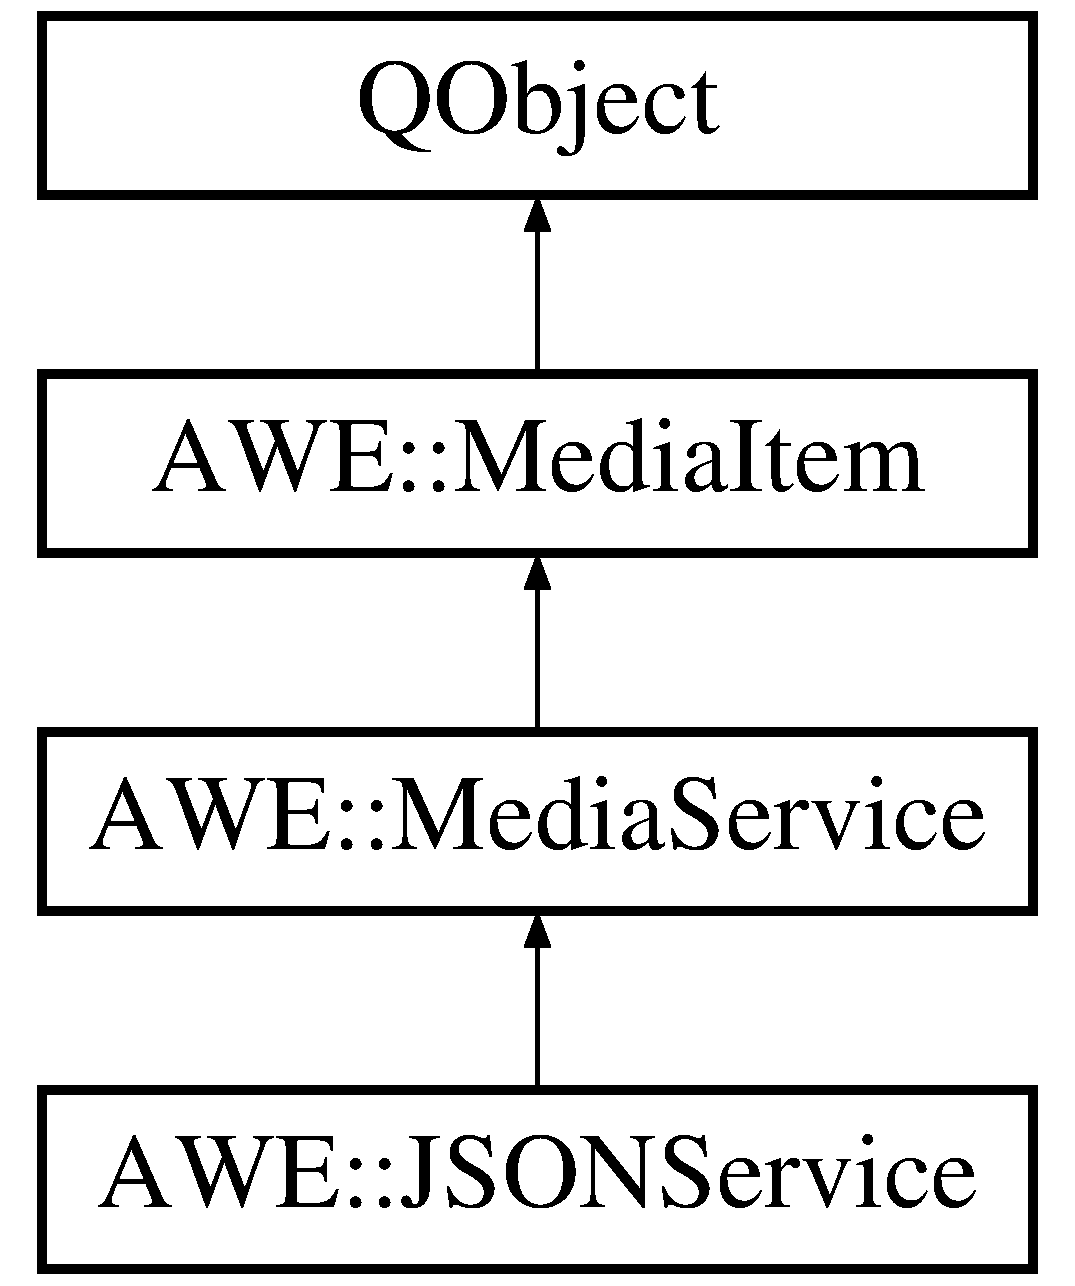
\includegraphics[height=3.000000cm]{class_a_w_e_1_1_j_s_o_n_service}
\end{center}
\end{figure}
\subsection*{Public Member Functions}
\begin{DoxyCompactItemize}
\item 
\hyperlink{class_a_w_e_1_1_j_s_o_n_service_a58c3b9fa5381f96db275cc3231dc4f83}{J\-S\-O\-N\-Service} (const Q\-Dir \&file)
\begin{DoxyCompactList}\small\item\em Construct an \hyperlink{class_a_w_e_1_1_media_service}{Media\-Service} from its J\-S\-O\-N file. \end{DoxyCompactList}\item 
virtual int \hyperlink{class_a_w_e_1_1_j_s_o_n_service_a19bbb59a75a05ad22d768d73febeeeda}{open} ()
\begin{DoxyCompactList}\small\item\em Open the application. \end{DoxyCompactList}\end{DoxyCompactItemize}
\subsection*{Additional Inherited Members}


\subsection{Detailed Description}
An external media service (aka application) described by a J\-S\-O\-N file. 

\subsection{Constructor \& Destructor Documentation}
\hypertarget{class_a_w_e_1_1_j_s_o_n_service_a58c3b9fa5381f96db275cc3231dc4f83}{\index{A\-W\-E\-::\-J\-S\-O\-N\-Service@{A\-W\-E\-::\-J\-S\-O\-N\-Service}!J\-S\-O\-N\-Service@{J\-S\-O\-N\-Service}}
\index{J\-S\-O\-N\-Service@{J\-S\-O\-N\-Service}!AWE::JSONService@{A\-W\-E\-::\-J\-S\-O\-N\-Service}}
\subsubsection[{J\-S\-O\-N\-Service}]{\setlength{\rightskip}{0pt plus 5cm}J\-S\-O\-N\-Service\-::\-J\-S\-O\-N\-Service (
\begin{DoxyParamCaption}
\item[{const Q\-Dir \&}]{file}
\end{DoxyParamCaption}
)}}\label{class_a_w_e_1_1_j_s_o_n_service_a58c3b9fa5381f96db275cc3231dc4f83}


Construct an \hyperlink{class_a_w_e_1_1_media_service}{Media\-Service} from its J\-S\-O\-N file. 


\begin{DoxyParams}{Parameters}
{\em file} & The J\-S\-O\-N file. \\
\hline
\end{DoxyParams}


\subsection{Member Function Documentation}
\hypertarget{class_a_w_e_1_1_j_s_o_n_service_a19bbb59a75a05ad22d768d73febeeeda}{\index{A\-W\-E\-::\-J\-S\-O\-N\-Service@{A\-W\-E\-::\-J\-S\-O\-N\-Service}!open@{open}}
\index{open@{open}!AWE::JSONService@{A\-W\-E\-::\-J\-S\-O\-N\-Service}}
\subsubsection[{open}]{\setlength{\rightskip}{0pt plus 5cm}int J\-S\-O\-N\-Service\-::open (
\begin{DoxyParamCaption}
{}
\end{DoxyParamCaption}
)\hspace{0.3cm}{\ttfamily [virtual]}}}\label{class_a_w_e_1_1_j_s_o_n_service_a19bbb59a75a05ad22d768d73febeeeda}


Open the application. 

\begin{DoxyReturn}{Returns}
The exit code of the application. 
\end{DoxyReturn}


Implements \hyperlink{class_a_w_e_1_1_media_service_ad13c100468482ce42880941bbeca4623}{A\-W\-E\-::\-Media\-Service}.



The documentation for this class was generated from the following files\-:\begin{DoxyCompactItemize}
\item 
/\-Users/\-Alex/github/\-A\-W\-E\-Media\-Center/\-Code/items/A\-W\-E\-J\-S\-O\-N\-Service.\-h\item 
/\-Users/\-Alex/github/\-A\-W\-E\-Media\-Center/\-Code/items/A\-W\-E\-J\-S\-O\-N\-Service.\-cpp\end{DoxyCompactItemize}

\hypertarget{class_a_w_e_1_1_media_file}{\section{A\-W\-E\-:\-:Media\-File Class Reference}
\label{class_a_w_e_1_1_media_file}\index{A\-W\-E\-::\-Media\-File@{A\-W\-E\-::\-Media\-File}}
}


Represents a media file.  




{\ttfamily \#include $<$A\-W\-E\-Media\-File.\-h$>$}

Inheritance diagram for A\-W\-E\-:\-:Media\-File\-:\begin{figure}[H]
\begin{center}
\leavevmode
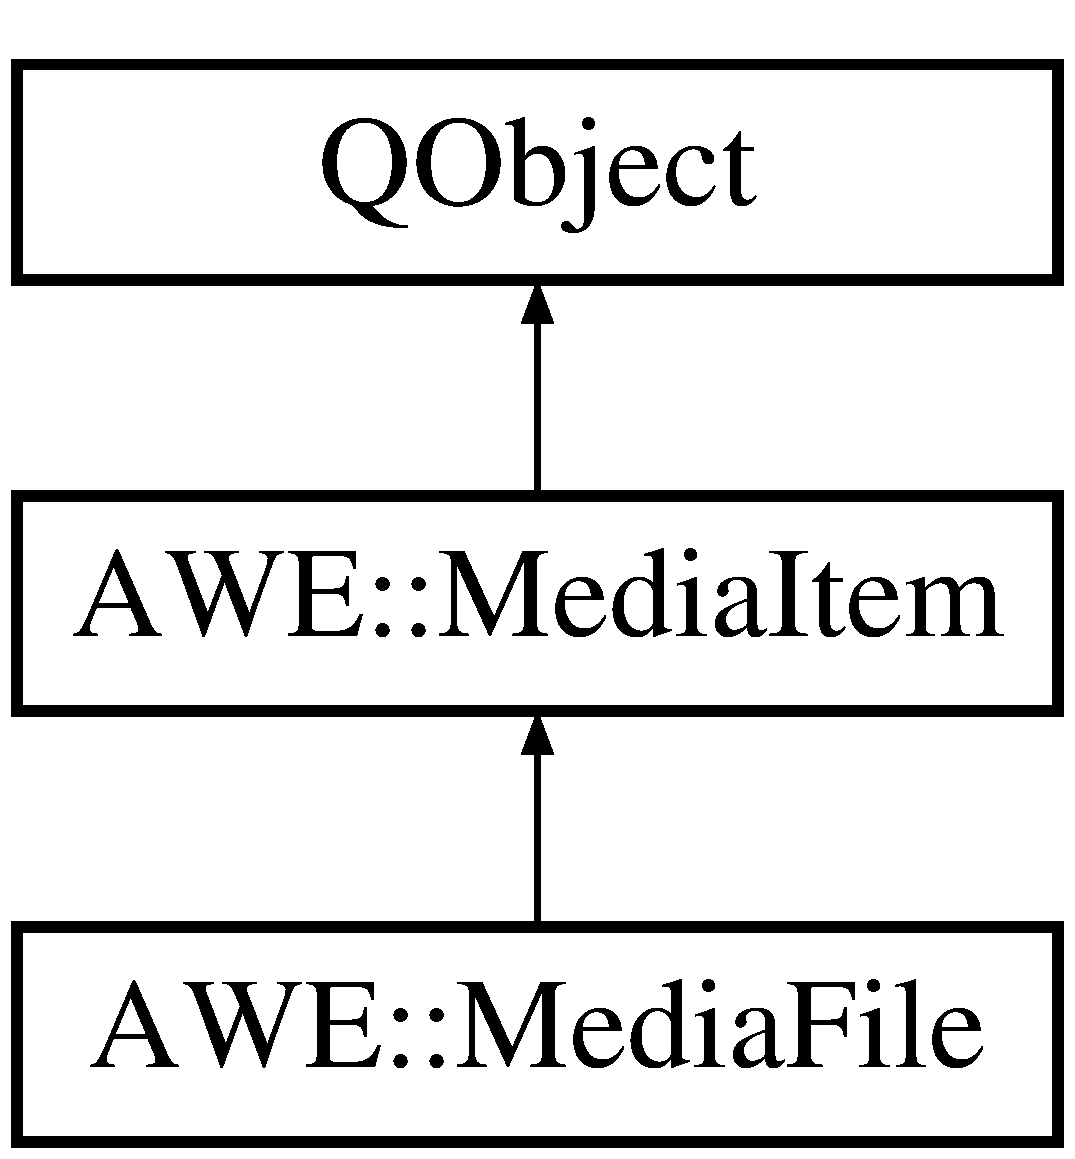
\includegraphics[height=3.000000cm]{class_a_w_e_1_1_media_file}
\end{center}
\end{figure}
\subsection*{Public Member Functions}
\begin{DoxyCompactItemize}
\item 
\hyperlink{class_a_w_e_1_1_media_file_af107afc7258da6cbadce1330bb9697a5}{Media\-File} (Q\-Dir file)
\begin{DoxyCompactList}\small\item\em Construct using the J\-S\-O\-N file. \end{DoxyCompactList}\item 
\hypertarget{class_a_w_e_1_1_media_file_a0ce25306ecf5a24c21dc3540d6293566}{virtual \hyperlink{class_a_w_e_1_1_media_file_a0ce25306ecf5a24c21dc3540d6293566}{$\sim$\-Media\-File} ()}\label{class_a_w_e_1_1_media_file_a0ce25306ecf5a24c21dc3540d6293566}

\begin{DoxyCompactList}\small\item\em Deconstructor. \end{DoxyCompactList}\item 
virtual Q\-Dir \hyperlink{class_a_w_e_1_1_media_file_a998b1415a248cf1915c7ff2b48af8586}{get\-Media\-File} () const 
\begin{DoxyCompactList}\small\item\em Get the absolute path to the media file. \end{DoxyCompactList}\item 
virtual \hyperlink{class_a_w_e_1_1_media_player}{Media\-Player} $\ast$ \hyperlink{class_a_w_e_1_1_media_file_a721cb652605a6cbc17a42899d9909079}{get\-Default\-Player} ()
\begin{DoxyCompactList}\small\item\em Get the default media player for this item. \end{DoxyCompactList}\item 
virtual int \hyperlink{class_a_w_e_1_1_media_file_a04870b77386642ea6568918f8d2693a2}{play} ()
\begin{DoxyCompactList}\small\item\em Play this item with the default player. \end{DoxyCompactList}\item 
virtual \hyperlink{namespace_a_w_e_ad175a5b8a86bf7848825c9bd94c41470}{Item\-Type} \hyperlink{class_a_w_e_1_1_media_file_a135ea553d8a72ec3c87b75281768ca69}{get\-Item\-Type} () const 
\begin{DoxyCompactList}\small\item\em Determine the basic type (folder, file, service) \end{DoxyCompactList}\end{DoxyCompactItemize}
\subsection*{Private Attributes}
\begin{DoxyCompactItemize}
\item 
\hypertarget{class_a_w_e_1_1_media_file_a546092fa2daee659f784573aa9fcdf99}{Q\-Dir \hyperlink{class_a_w_e_1_1_media_file_a546092fa2daee659f784573aa9fcdf99}{my\-Media\-File}}\label{class_a_w_e_1_1_media_file_a546092fa2daee659f784573aa9fcdf99}

\begin{DoxyCompactList}\small\item\em The path to the media file. \end{DoxyCompactList}\item 
\hypertarget{class_a_w_e_1_1_media_file_a86d064b6ab12e4eaade8e9cb32e0b595}{\hyperlink{class_a_w_e_1_1_media_player}{Media\-Player} $\ast$ \hyperlink{class_a_w_e_1_1_media_file_a86d064b6ab12e4eaade8e9cb32e0b595}{my\-Default\-Player}}\label{class_a_w_e_1_1_media_file_a86d064b6ab12e4eaade8e9cb32e0b595}

\begin{DoxyCompactList}\small\item\em The default media player. \end{DoxyCompactList}\end{DoxyCompactItemize}
\subsection*{Additional Inherited Members}


\subsection{Detailed Description}
Represents a media file. 

Holds the default player and all relevant metadata. 

\subsection{Constructor \& Destructor Documentation}
\hypertarget{class_a_w_e_1_1_media_file_af107afc7258da6cbadce1330bb9697a5}{\index{A\-W\-E\-::\-Media\-File@{A\-W\-E\-::\-Media\-File}!Media\-File@{Media\-File}}
\index{Media\-File@{Media\-File}!AWE::MediaFile@{A\-W\-E\-::\-Media\-File}}
\subsubsection[{Media\-File}]{\setlength{\rightskip}{0pt plus 5cm}Media\-File\-::\-Media\-File (
\begin{DoxyParamCaption}
\item[{Q\-Dir}]{file}
\end{DoxyParamCaption}
)}}\label{class_a_w_e_1_1_media_file_af107afc7258da6cbadce1330bb9697a5}


Construct using the J\-S\-O\-N file. 


\begin{DoxyParams}{Parameters}
{\em file} & The path to the file. \\
\hline
\end{DoxyParams}


\subsection{Member Function Documentation}
\hypertarget{class_a_w_e_1_1_media_file_a721cb652605a6cbc17a42899d9909079}{\index{A\-W\-E\-::\-Media\-File@{A\-W\-E\-::\-Media\-File}!get\-Default\-Player@{get\-Default\-Player}}
\index{get\-Default\-Player@{get\-Default\-Player}!AWE::MediaFile@{A\-W\-E\-::\-Media\-File}}
\subsubsection[{get\-Default\-Player}]{\setlength{\rightskip}{0pt plus 5cm}{\bf Media\-Player} $\ast$ Media\-File\-::get\-Default\-Player (
\begin{DoxyParamCaption}
{}
\end{DoxyParamCaption}
)\hspace{0.3cm}{\ttfamily [virtual]}}}\label{class_a_w_e_1_1_media_file_a721cb652605a6cbc17a42899d9909079}


Get the default media player for this item. 

\begin{DoxyReturn}{Returns}
The default media player for this item. 
\end{DoxyReturn}
\hypertarget{class_a_w_e_1_1_media_file_a135ea553d8a72ec3c87b75281768ca69}{\index{A\-W\-E\-::\-Media\-File@{A\-W\-E\-::\-Media\-File}!get\-Item\-Type@{get\-Item\-Type}}
\index{get\-Item\-Type@{get\-Item\-Type}!AWE::MediaFile@{A\-W\-E\-::\-Media\-File}}
\subsubsection[{get\-Item\-Type}]{\setlength{\rightskip}{0pt plus 5cm}{\bf Item\-Type} Media\-File\-::get\-Item\-Type (
\begin{DoxyParamCaption}
{}
\end{DoxyParamCaption}
) const\hspace{0.3cm}{\ttfamily [virtual]}}}\label{class_a_w_e_1_1_media_file_a135ea553d8a72ec3c87b75281768ca69}


Determine the basic type (folder, file, service) 

\begin{DoxyReturn}{Returns}
The basic type of this item. 
\end{DoxyReturn}


Implements \hyperlink{class_a_w_e_1_1_media_item_ad7a7ef28069986fad8b2be060fef6e48}{A\-W\-E\-::\-Media\-Item}.

\hypertarget{class_a_w_e_1_1_media_file_a998b1415a248cf1915c7ff2b48af8586}{\index{A\-W\-E\-::\-Media\-File@{A\-W\-E\-::\-Media\-File}!get\-Media\-File@{get\-Media\-File}}
\index{get\-Media\-File@{get\-Media\-File}!AWE::MediaFile@{A\-W\-E\-::\-Media\-File}}
\subsubsection[{get\-Media\-File}]{\setlength{\rightskip}{0pt plus 5cm}Q\-Dir Media\-File\-::get\-Media\-File (
\begin{DoxyParamCaption}
{}
\end{DoxyParamCaption}
) const\hspace{0.3cm}{\ttfamily [virtual]}}}\label{class_a_w_e_1_1_media_file_a998b1415a248cf1915c7ff2b48af8586}


Get the absolute path to the media file. 

\begin{DoxyReturn}{Returns}
The absolute path to of the media file. 
\end{DoxyReturn}
\hypertarget{class_a_w_e_1_1_media_file_a04870b77386642ea6568918f8d2693a2}{\index{A\-W\-E\-::\-Media\-File@{A\-W\-E\-::\-Media\-File}!play@{play}}
\index{play@{play}!AWE::MediaFile@{A\-W\-E\-::\-Media\-File}}
\subsubsection[{play}]{\setlength{\rightskip}{0pt plus 5cm}int Media\-File\-::play (
\begin{DoxyParamCaption}
{}
\end{DoxyParamCaption}
)\hspace{0.3cm}{\ttfamily [virtual]}}}\label{class_a_w_e_1_1_media_file_a04870b77386642ea6568918f8d2693a2}


Play this item with the default player. 

\begin{DoxyReturn}{Returns}
{\ttfamily true} if playback was successful, {\ttfamily false} if it was not. 
\end{DoxyReturn}


The documentation for this class was generated from the following files\-:\begin{DoxyCompactItemize}
\item 
/\-Users/\-Alex/github/\-A\-W\-E\-Media\-Center/\-Code/items/A\-W\-E\-Media\-File.\-h\item 
/\-Users/\-Alex/github/\-A\-W\-E\-Media\-Center/\-Code/items/A\-W\-E\-Media\-File.\-cpp\end{DoxyCompactItemize}

\hypertarget{class_a_w_e_1_1_media_item}{\section{A\-W\-E\-:\-:Media\-Item Class Reference}
\label{class_a_w_e_1_1_media_item}\index{A\-W\-E\-::\-Media\-Item@{A\-W\-E\-::\-Media\-Item}}
}


Represents a media file, folder, or service.  




{\ttfamily \#include $<$A\-W\-E\-Media\-Item.\-h$>$}

Inheritance diagram for A\-W\-E\-:\-:Media\-Item\-:\begin{figure}[H]
\begin{center}
\leavevmode
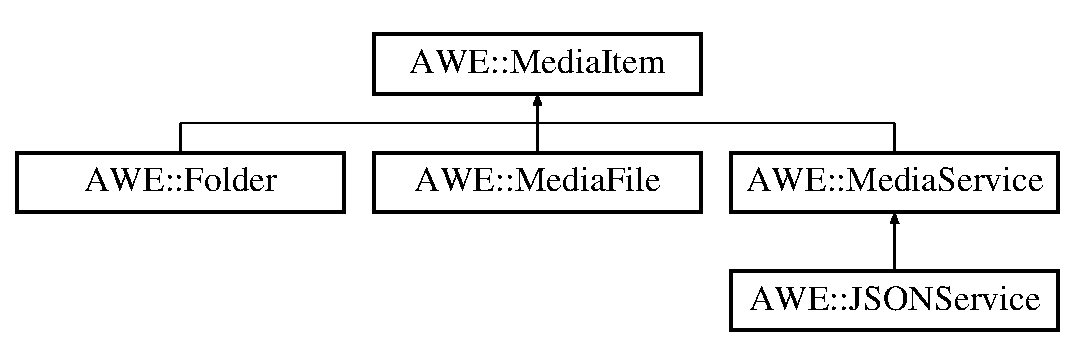
\includegraphics[height=3.000000cm]{class_a_w_e_1_1_media_item}
\end{center}
\end{figure}
\subsection*{Public Member Functions}
\begin{DoxyCompactItemize}
\item 
\hyperlink{class_a_w_e_1_1_media_item_a8cb8aeb690c2833d5bc175d40a1f7fe6}{Media\-Item} (const Q\-Dir \&file)
\begin{DoxyCompactList}\small\item\em Create from the given J\-S\-O\-N file. \end{DoxyCompactList}\item 
\hypertarget{class_a_w_e_1_1_media_item_a6999ea20d13e6fcd55b2d4104ca15b78}{virtual \hyperlink{class_a_w_e_1_1_media_item_a6999ea20d13e6fcd55b2d4104ca15b78}{$\sim$\-Media\-Item} ()}\label{class_a_w_e_1_1_media_item_a6999ea20d13e6fcd55b2d4104ca15b78}

\begin{DoxyCompactList}\small\item\em Deconstructor. \end{DoxyCompactList}\item 
virtual \hyperlink{class_json_1_1_value}{Json\-::\-Value} \& \hyperlink{class_a_w_e_1_1_media_item_ac3258f4f7f4557205b3906ff15c46612}{get\-Data} ()
\begin{DoxyCompactList}\small\item\em Get the data for this item. \end{DoxyCompactList}\item 
virtual const \hyperlink{class_json_1_1_value}{Json\-::\-Value} \& \hyperlink{class_a_w_e_1_1_media_item_abd79979e34b76f89d6cadabcb7886bd1}{get\-Data} () const 
\begin{DoxyCompactList}\small\item\em Get the data for this item. \end{DoxyCompactList}\item 
virtual const \hyperlink{class_json_1_1_value}{Json\-::\-Value} \& \hyperlink{class_a_w_e_1_1_media_item_a82bd831701d2a4c727ff505fbf9fbbb0}{get\-Member} (const std\-::string \&str) const 
\begin{DoxyCompactList}\small\item\em Get a member of unspecified type by name. \end{DoxyCompactList}\item 
virtual \hyperlink{class_json_1_1_value}{Json\-::\-Value} \& \hyperlink{class_a_w_e_1_1_media_item_a64bf0d84b75bd21dd27ef498c85bf695}{get\-Member} (const std\-::string \&str)
\begin{DoxyCompactList}\small\item\em Get a member of unspecified type by name. \end{DoxyCompactList}\item 
virtual bool \hyperlink{class_a_w_e_1_1_media_item_ad0beee6cac6524de24f5a1449502cdd5}{get\-Bool\-Member} (const std\-::string \&str) const 
\begin{DoxyCompactList}\small\item\em Get a member of {\ttfamily bool} type by name. \end{DoxyCompactList}\item 
virtual std\-::string \hyperlink{class_a_w_e_1_1_media_item_a86775a7b5252062953963840b3074568}{get\-String\-Member} (const std\-::string \&str) const 
\begin{DoxyCompactList}\small\item\em Get a member of {\ttfamily std\-::string} type by name. \end{DoxyCompactList}\item 
virtual int \hyperlink{class_a_w_e_1_1_media_item_a18ac2a793896f54695f4796f8457b073}{get\-Int\-Member} (const std\-::string \&str) const 
\begin{DoxyCompactList}\small\item\em Get a member of {\ttfamily int} type by name. \end{DoxyCompactList}\item 
virtual std\-::string \hyperlink{class_a_w_e_1_1_media_item_a20a3275880777c9c5338957ee5d2d1e1}{get\-Name} () const 
\begin{DoxyCompactList}\small\item\em Get the name of the media item. \end{DoxyCompactList}\item 
virtual const Q\-Dir \& \hyperlink{class_a_w_e_1_1_media_item_a6a26f1692daa54667f4efd3f89c2769d}{get\-J\-S\-O\-N\-File} () const 
\begin{DoxyCompactList}\small\item\em Get the absolute path to the J\-S\-O\-N settings file. \end{DoxyCompactList}\item 
virtual Item\-Type \hyperlink{class_a_w_e_1_1_media_item_ad7a7ef28069986fad8b2be060fef6e48}{get\-Item\-Type} () const =0
\begin{DoxyCompactList}\small\item\em Determine the basic type (folder, file, service) \end{DoxyCompactList}\end{DoxyCompactItemize}
\subsection*{Protected Attributes}
\begin{DoxyCompactItemize}
\item 
\hypertarget{class_a_w_e_1_1_media_item_a7f9dd23352cad06e432264b85e58778d}{Q\-Dir \hyperlink{class_a_w_e_1_1_media_item_a7f9dd23352cad06e432264b85e58778d}{my\-J\-S\-O\-N\-File}}\label{class_a_w_e_1_1_media_item_a7f9dd23352cad06e432264b85e58778d}

\begin{DoxyCompactList}\small\item\em The J\-S\-O\-N file for this item. \end{DoxyCompactList}\item 
\hypertarget{class_a_w_e_1_1_media_item_a7af1109bed3163e1c5a33aac5d369ad8}{\hyperlink{class_json_1_1_value}{Json\-::\-Value} \hyperlink{class_a_w_e_1_1_media_item_a7af1109bed3163e1c5a33aac5d369ad8}{my\-Data}}\label{class_a_w_e_1_1_media_item_a7af1109bed3163e1c5a33aac5d369ad8}

\begin{DoxyCompactList}\small\item\em The data for this item. \end{DoxyCompactList}\end{DoxyCompactItemize}


\subsection{Detailed Description}
Represents a media file, folder, or service. 

Holds all relevant metadata for the item. 

\subsection{Constructor \& Destructor Documentation}
\hypertarget{class_a_w_e_1_1_media_item_a8cb8aeb690c2833d5bc175d40a1f7fe6}{\index{A\-W\-E\-::\-Media\-Item@{A\-W\-E\-::\-Media\-Item}!Media\-Item@{Media\-Item}}
\index{Media\-Item@{Media\-Item}!AWE::MediaItem@{A\-W\-E\-::\-Media\-Item}}
\subsubsection[{Media\-Item}]{\setlength{\rightskip}{0pt plus 5cm}Media\-Item\-::\-Media\-Item (
\begin{DoxyParamCaption}
\item[{const Q\-Dir \&}]{file}
\end{DoxyParamCaption}
)}}\label{class_a_w_e_1_1_media_item_a8cb8aeb690c2833d5bc175d40a1f7fe6}


Create from the given J\-S\-O\-N file. 


\begin{DoxyParams}{Parameters}
{\em file} & The J\-S\-O\-N file path. \\
\hline
\end{DoxyParams}


\subsection{Member Function Documentation}
\hypertarget{class_a_w_e_1_1_media_item_ad0beee6cac6524de24f5a1449502cdd5}{\index{A\-W\-E\-::\-Media\-Item@{A\-W\-E\-::\-Media\-Item}!get\-Bool\-Member@{get\-Bool\-Member}}
\index{get\-Bool\-Member@{get\-Bool\-Member}!AWE::MediaItem@{A\-W\-E\-::\-Media\-Item}}
\subsubsection[{get\-Bool\-Member}]{\setlength{\rightskip}{0pt plus 5cm}bool Media\-Item\-::get\-Bool\-Member (
\begin{DoxyParamCaption}
\item[{const std\-::string \&}]{str}
\end{DoxyParamCaption}
) const\hspace{0.3cm}{\ttfamily [virtual]}}}\label{class_a_w_e_1_1_media_item_ad0beee6cac6524de24f5a1449502cdd5}


Get a member of {\ttfamily bool} type by name. 


\begin{DoxyParams}{Parameters}
{\em str} & A formatted string representing the path to the member variable in the J\-S\-O\-N file.\\
\hline
\end{DoxyParams}
\begin{DoxyReturn}{Returns}
The value associated with the key {\ttfamily str}. 
\end{DoxyReturn}
\hypertarget{class_a_w_e_1_1_media_item_ac3258f4f7f4557205b3906ff15c46612}{\index{A\-W\-E\-::\-Media\-Item@{A\-W\-E\-::\-Media\-Item}!get\-Data@{get\-Data}}
\index{get\-Data@{get\-Data}!AWE::MediaItem@{A\-W\-E\-::\-Media\-Item}}
\subsubsection[{get\-Data}]{\setlength{\rightskip}{0pt plus 5cm}{\bf Value} \& Media\-Item\-::get\-Data (
\begin{DoxyParamCaption}
{}
\end{DoxyParamCaption}
)\hspace{0.3cm}{\ttfamily [virtual]}}}\label{class_a_w_e_1_1_media_item_ac3258f4f7f4557205b3906ff15c46612}


Get the data for this item. 

\begin{DoxyReturn}{Returns}
The data for this item. 
\end{DoxyReturn}
\hypertarget{class_a_w_e_1_1_media_item_abd79979e34b76f89d6cadabcb7886bd1}{\index{A\-W\-E\-::\-Media\-Item@{A\-W\-E\-::\-Media\-Item}!get\-Data@{get\-Data}}
\index{get\-Data@{get\-Data}!AWE::MediaItem@{A\-W\-E\-::\-Media\-Item}}
\subsubsection[{get\-Data}]{\setlength{\rightskip}{0pt plus 5cm}const {\bf Value} \& Media\-Item\-::get\-Data (
\begin{DoxyParamCaption}
{}
\end{DoxyParamCaption}
) const\hspace{0.3cm}{\ttfamily [virtual]}}}\label{class_a_w_e_1_1_media_item_abd79979e34b76f89d6cadabcb7886bd1}


Get the data for this item. 

\begin{DoxyReturn}{Returns}
The data for this item. 
\end{DoxyReturn}
\hypertarget{class_a_w_e_1_1_media_item_a18ac2a793896f54695f4796f8457b073}{\index{A\-W\-E\-::\-Media\-Item@{A\-W\-E\-::\-Media\-Item}!get\-Int\-Member@{get\-Int\-Member}}
\index{get\-Int\-Member@{get\-Int\-Member}!AWE::MediaItem@{A\-W\-E\-::\-Media\-Item}}
\subsubsection[{get\-Int\-Member}]{\setlength{\rightskip}{0pt plus 5cm}int Media\-Item\-::get\-Int\-Member (
\begin{DoxyParamCaption}
\item[{const std\-::string \&}]{str}
\end{DoxyParamCaption}
) const\hspace{0.3cm}{\ttfamily [virtual]}}}\label{class_a_w_e_1_1_media_item_a18ac2a793896f54695f4796f8457b073}


Get a member of {\ttfamily int} type by name. 


\begin{DoxyParams}{Parameters}
{\em str} & A formatted string representing the path to the member variable in the J\-S\-O\-N file.\\
\hline
\end{DoxyParams}
\begin{DoxyReturn}{Returns}
The value associated with the key {\ttfamily str}. 
\end{DoxyReturn}
\hypertarget{class_a_w_e_1_1_media_item_ad7a7ef28069986fad8b2be060fef6e48}{\index{A\-W\-E\-::\-Media\-Item@{A\-W\-E\-::\-Media\-Item}!get\-Item\-Type@{get\-Item\-Type}}
\index{get\-Item\-Type@{get\-Item\-Type}!AWE::MediaItem@{A\-W\-E\-::\-Media\-Item}}
\subsubsection[{get\-Item\-Type}]{\setlength{\rightskip}{0pt plus 5cm}virtual Item\-Type A\-W\-E\-::\-Media\-Item\-::get\-Item\-Type (
\begin{DoxyParamCaption}
{}
\end{DoxyParamCaption}
) const\hspace{0.3cm}{\ttfamily [pure virtual]}}}\label{class_a_w_e_1_1_media_item_ad7a7ef28069986fad8b2be060fef6e48}


Determine the basic type (folder, file, service) 

\begin{DoxyReturn}{Returns}
The basic type of this item. 
\end{DoxyReturn}


Implemented in \hyperlink{class_a_w_e_1_1_media_file_a135ea553d8a72ec3c87b75281768ca69}{A\-W\-E\-::\-Media\-File}, \hyperlink{class_a_w_e_1_1_folder_a315c0a52f6e37b357d5f0e4fc5526d52}{A\-W\-E\-::\-Folder}, and \hyperlink{class_a_w_e_1_1_media_service_a680d2f9fd50b27cb7156c3a5777dee12}{A\-W\-E\-::\-Media\-Service}.

\hypertarget{class_a_w_e_1_1_media_item_a6a26f1692daa54667f4efd3f89c2769d}{\index{A\-W\-E\-::\-Media\-Item@{A\-W\-E\-::\-Media\-Item}!get\-J\-S\-O\-N\-File@{get\-J\-S\-O\-N\-File}}
\index{get\-J\-S\-O\-N\-File@{get\-J\-S\-O\-N\-File}!AWE::MediaItem@{A\-W\-E\-::\-Media\-Item}}
\subsubsection[{get\-J\-S\-O\-N\-File}]{\setlength{\rightskip}{0pt plus 5cm}const Q\-Dir \& Media\-Item\-::get\-J\-S\-O\-N\-File (
\begin{DoxyParamCaption}
{}
\end{DoxyParamCaption}
) const\hspace{0.3cm}{\ttfamily [virtual]}}}\label{class_a_w_e_1_1_media_item_a6a26f1692daa54667f4efd3f89c2769d}


Get the absolute path to the J\-S\-O\-N settings file. 

\begin{DoxyReturn}{Returns}
The path to the J\-S\-O\-N settings file. 
\end{DoxyReturn}
\hypertarget{class_a_w_e_1_1_media_item_a82bd831701d2a4c727ff505fbf9fbbb0}{\index{A\-W\-E\-::\-Media\-Item@{A\-W\-E\-::\-Media\-Item}!get\-Member@{get\-Member}}
\index{get\-Member@{get\-Member}!AWE::MediaItem@{A\-W\-E\-::\-Media\-Item}}
\subsubsection[{get\-Member}]{\setlength{\rightskip}{0pt plus 5cm}const {\bf Value} \& Media\-Item\-::get\-Member (
\begin{DoxyParamCaption}
\item[{const std\-::string \&}]{str}
\end{DoxyParamCaption}
) const\hspace{0.3cm}{\ttfamily [virtual]}}}\label{class_a_w_e_1_1_media_item_a82bd831701d2a4c727ff505fbf9fbbb0}


Get a member of unspecified type by name. 


\begin{DoxyParams}{Parameters}
{\em str} & A formatted string representing the path to the member variable in the J\-S\-O\-N file.\\
\hline
\end{DoxyParams}
\begin{DoxyReturn}{Returns}
The value associated with the key {\ttfamily str}. 
\end{DoxyReturn}
\hypertarget{class_a_w_e_1_1_media_item_a64bf0d84b75bd21dd27ef498c85bf695}{\index{A\-W\-E\-::\-Media\-Item@{A\-W\-E\-::\-Media\-Item}!get\-Member@{get\-Member}}
\index{get\-Member@{get\-Member}!AWE::MediaItem@{A\-W\-E\-::\-Media\-Item}}
\subsubsection[{get\-Member}]{\setlength{\rightskip}{0pt plus 5cm}{\bf Value} \& Media\-Item\-::get\-Member (
\begin{DoxyParamCaption}
\item[{const std\-::string \&}]{str}
\end{DoxyParamCaption}
)\hspace{0.3cm}{\ttfamily [virtual]}}}\label{class_a_w_e_1_1_media_item_a64bf0d84b75bd21dd27ef498c85bf695}


Get a member of unspecified type by name. 


\begin{DoxyParams}{Parameters}
{\em str} & A formatted string representing the path to the member variable in the J\-S\-O\-N file.\\
\hline
\end{DoxyParams}
\begin{DoxyReturn}{Returns}
The value associated with the key {\ttfamily str}. 
\end{DoxyReturn}
\hypertarget{class_a_w_e_1_1_media_item_a20a3275880777c9c5338957ee5d2d1e1}{\index{A\-W\-E\-::\-Media\-Item@{A\-W\-E\-::\-Media\-Item}!get\-Name@{get\-Name}}
\index{get\-Name@{get\-Name}!AWE::MediaItem@{A\-W\-E\-::\-Media\-Item}}
\subsubsection[{get\-Name}]{\setlength{\rightskip}{0pt plus 5cm}std\-::string Media\-Item\-::get\-Name (
\begin{DoxyParamCaption}
{}
\end{DoxyParamCaption}
) const\hspace{0.3cm}{\ttfamily [virtual]}}}\label{class_a_w_e_1_1_media_item_a20a3275880777c9c5338957ee5d2d1e1}


Get the name of the media item. 

Equivalent to {\ttfamily get\-String\-Member(\char`\"{}metadata.\-name\char`\"{})}

\begin{DoxyReturn}{Returns}
The name of this media item. 
\end{DoxyReturn}
\hypertarget{class_a_w_e_1_1_media_item_a86775a7b5252062953963840b3074568}{\index{A\-W\-E\-::\-Media\-Item@{A\-W\-E\-::\-Media\-Item}!get\-String\-Member@{get\-String\-Member}}
\index{get\-String\-Member@{get\-String\-Member}!AWE::MediaItem@{A\-W\-E\-::\-Media\-Item}}
\subsubsection[{get\-String\-Member}]{\setlength{\rightskip}{0pt plus 5cm}std\-::string Media\-Item\-::get\-String\-Member (
\begin{DoxyParamCaption}
\item[{const std\-::string \&}]{str}
\end{DoxyParamCaption}
) const\hspace{0.3cm}{\ttfamily [virtual]}}}\label{class_a_w_e_1_1_media_item_a86775a7b5252062953963840b3074568}


Get a member of {\ttfamily std\-::string} type by name. 


\begin{DoxyParams}{Parameters}
{\em str} & A formatted string representing the path to the member variable in the J\-S\-O\-N file.\\
\hline
\end{DoxyParams}
\begin{DoxyReturn}{Returns}
The value associated with the key {\ttfamily str}. 
\end{DoxyReturn}


The documentation for this class was generated from the following files\-:\begin{DoxyCompactItemize}
\item 
/\-Users/\-Alex/github/\-A\-W\-E\-Media\-Center/\-Code/items/A\-W\-E\-Media\-Item.\-h\item 
/\-Users/\-Alex/github/\-A\-W\-E\-Media\-Center/\-Code/items/A\-W\-E\-Media\-Item.\-cpp\end{DoxyCompactItemize}

\hypertarget{class_a_w_e_1_1_media_player}{\section{A\-W\-E\-:\-:Media\-Player Class Reference}
\label{class_a_w_e_1_1_media_player}\index{A\-W\-E\-::\-Media\-Player@{A\-W\-E\-::\-Media\-Player}}
}


Represents an abstract media player's functions.  




{\ttfamily \#include $<$A\-W\-E\-Media\-Player.\-h$>$}

Inheritance diagram for A\-W\-E\-:\-:Media\-Player\-:\begin{figure}[H]
\begin{center}
\leavevmode
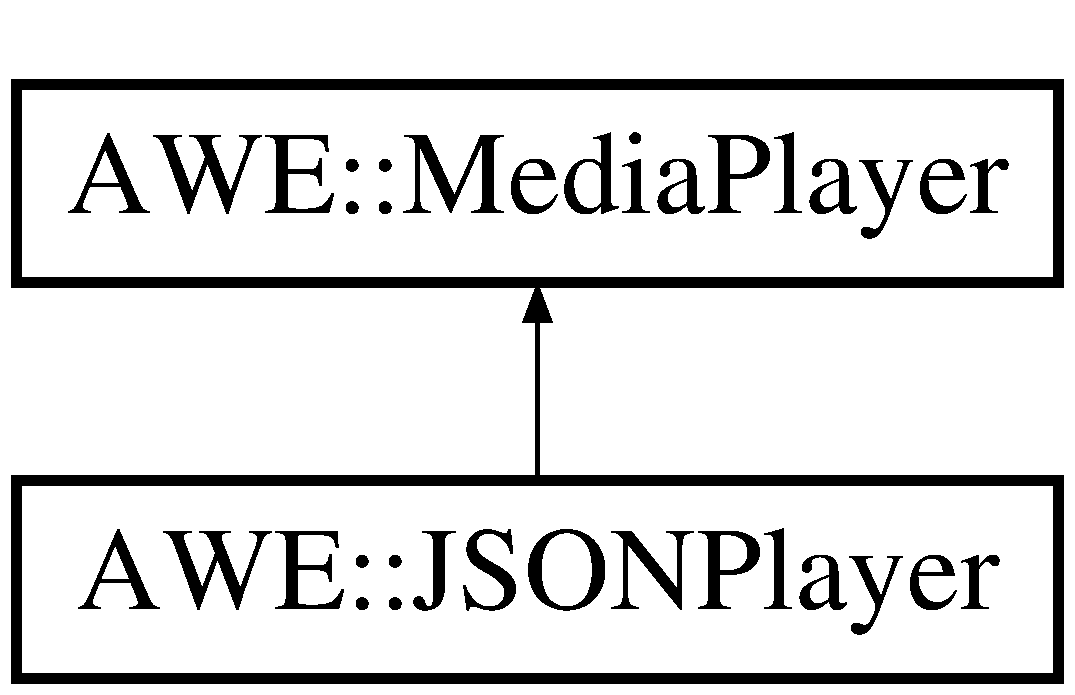
\includegraphics[height=2.000000cm]{class_a_w_e_1_1_media_player}
\end{center}
\end{figure}
\subsection*{Public Member Functions}
\begin{DoxyCompactItemize}
\item 
\hypertarget{class_a_w_e_1_1_media_player_af4e56a79d4ee564e0337a6b5c0bbf592}{virtual \hyperlink{class_a_w_e_1_1_media_player_af4e56a79d4ee564e0337a6b5c0bbf592}{$\sim$\-Media\-Player} ()}\label{class_a_w_e_1_1_media_player_af4e56a79d4ee564e0337a6b5c0bbf592}

\begin{DoxyCompactList}\small\item\em Deconstructor. \end{DoxyCompactList}\item 
virtual int \hyperlink{class_a_w_e_1_1_media_player_a8a7660cdf7306adf61a7c79831ee7171}{play} (\hyperlink{class_a_w_e_1_1_media_file}{Media\-File} $\ast$file)=0
\begin{DoxyCompactList}\small\item\em Play the given file. \end{DoxyCompactList}\item 
virtual Q\-String \hyperlink{class_a_w_e_1_1_media_player_a481bc1288b8b3bde9c5116d7ffd3c2f2}{get\-Name} () const =0
\begin{DoxyCompactList}\small\item\em Get the name of the player. \end{DoxyCompactList}\item 
virtual bool \hyperlink{class_a_w_e_1_1_media_player_a8dd37e3307cef837b296f94e4b398138}{can\-Play} (\hyperlink{class_a_w_e_1_1_media_file}{Media\-File} $\ast$file)=0
\begin{DoxyCompactList}\small\item\em Determine if the given media file can be played by this player. \end{DoxyCompactList}\end{DoxyCompactItemize}


\subsection{Detailed Description}
Represents an abstract media player's functions. 

\begin{DoxyRefDesc}{Todo}
\item[\hyperlink{todo__todo000001}{Todo}]Make plugin interface. \end{DoxyRefDesc}


\subsection{Member Function Documentation}
\hypertarget{class_a_w_e_1_1_media_player_a8dd37e3307cef837b296f94e4b398138}{\index{A\-W\-E\-::\-Media\-Player@{A\-W\-E\-::\-Media\-Player}!can\-Play@{can\-Play}}
\index{can\-Play@{can\-Play}!AWE::MediaPlayer@{A\-W\-E\-::\-Media\-Player}}
\subsubsection[{can\-Play}]{\setlength{\rightskip}{0pt plus 5cm}virtual bool A\-W\-E\-::\-Media\-Player\-::can\-Play (
\begin{DoxyParamCaption}
\item[{{\bf Media\-File} $\ast$}]{file}
\end{DoxyParamCaption}
)\hspace{0.3cm}{\ttfamily [pure virtual]}}}\label{class_a_w_e_1_1_media_player_a8dd37e3307cef837b296f94e4b398138}


Determine if the given media file can be played by this player. 


\begin{DoxyParams}{Parameters}
{\em file} & The file to determine playability for.\\
\hline
\end{DoxyParams}
\begin{DoxyReturn}{Returns}
{\ttfamily true} if this player can play {\ttfamily file}, {\ttfamily false} otherwise. 
\end{DoxyReturn}


Implemented in \hyperlink{class_a_w_e_1_1_j_s_o_n_player_adba5012e59f5d77f0e08fafeaac017fa}{A\-W\-E\-::\-J\-S\-O\-N\-Player}.

\hypertarget{class_a_w_e_1_1_media_player_a481bc1288b8b3bde9c5116d7ffd3c2f2}{\index{A\-W\-E\-::\-Media\-Player@{A\-W\-E\-::\-Media\-Player}!get\-Name@{get\-Name}}
\index{get\-Name@{get\-Name}!AWE::MediaPlayer@{A\-W\-E\-::\-Media\-Player}}
\subsubsection[{get\-Name}]{\setlength{\rightskip}{0pt plus 5cm}virtual Q\-String A\-W\-E\-::\-Media\-Player\-::get\-Name (
\begin{DoxyParamCaption}
{}
\end{DoxyParamCaption}
) const\hspace{0.3cm}{\ttfamily [pure virtual]}}}\label{class_a_w_e_1_1_media_player_a481bc1288b8b3bde9c5116d7ffd3c2f2}


Get the name of the player. 

\begin{DoxyReturn}{Returns}
The name of the player. 
\end{DoxyReturn}


Implemented in \hyperlink{class_a_w_e_1_1_j_s_o_n_player_a9d65a8aa1003452e607ecb481adfb79e}{A\-W\-E\-::\-J\-S\-O\-N\-Player}.

\hypertarget{class_a_w_e_1_1_media_player_a8a7660cdf7306adf61a7c79831ee7171}{\index{A\-W\-E\-::\-Media\-Player@{A\-W\-E\-::\-Media\-Player}!play@{play}}
\index{play@{play}!AWE::MediaPlayer@{A\-W\-E\-::\-Media\-Player}}
\subsubsection[{play}]{\setlength{\rightskip}{0pt plus 5cm}virtual int A\-W\-E\-::\-Media\-Player\-::play (
\begin{DoxyParamCaption}
\item[{{\bf Media\-File} $\ast$}]{file}
\end{DoxyParamCaption}
)\hspace{0.3cm}{\ttfamily [pure virtual]}}}\label{class_a_w_e_1_1_media_player_a8a7660cdf7306adf61a7c79831ee7171}


Play the given file. 


\begin{DoxyParams}{Parameters}
{\em file} & The media file to play.\\
\hline
\end{DoxyParams}
\begin{DoxyReturn}{Returns}
{\ttfamily true} if {\ttfamily file} played successfully, {\ttfamily false} otherwise. 
\end{DoxyReturn}


Implemented in \hyperlink{class_a_w_e_1_1_j_s_o_n_player_a417957c7b0826ecef28b232a2cf9d49e}{A\-W\-E\-::\-J\-S\-O\-N\-Player}.



The documentation for this class was generated from the following file\-:\begin{DoxyCompactItemize}
\item 
/\-Users/\-Alex/github/\-A\-W\-E\-Media\-Center/\-Code/player/A\-W\-E\-Media\-Player.\-h\end{DoxyCompactItemize}

\hypertarget{class_a_w_e_1_1_media_service}{\section{A\-W\-E\-:\-:Media\-Service Class Reference}
\label{class_a_w_e_1_1_media_service}\index{A\-W\-E\-::\-Media\-Service@{A\-W\-E\-::\-Media\-Service}}
}


A media service, which is basically an application with its own media browser.  




{\ttfamily \#include $<$A\-W\-E\-Media\-Service.\-h$>$}

Inheritance diagram for A\-W\-E\-:\-:Media\-Service\-:\begin{figure}[H]
\begin{center}
\leavevmode
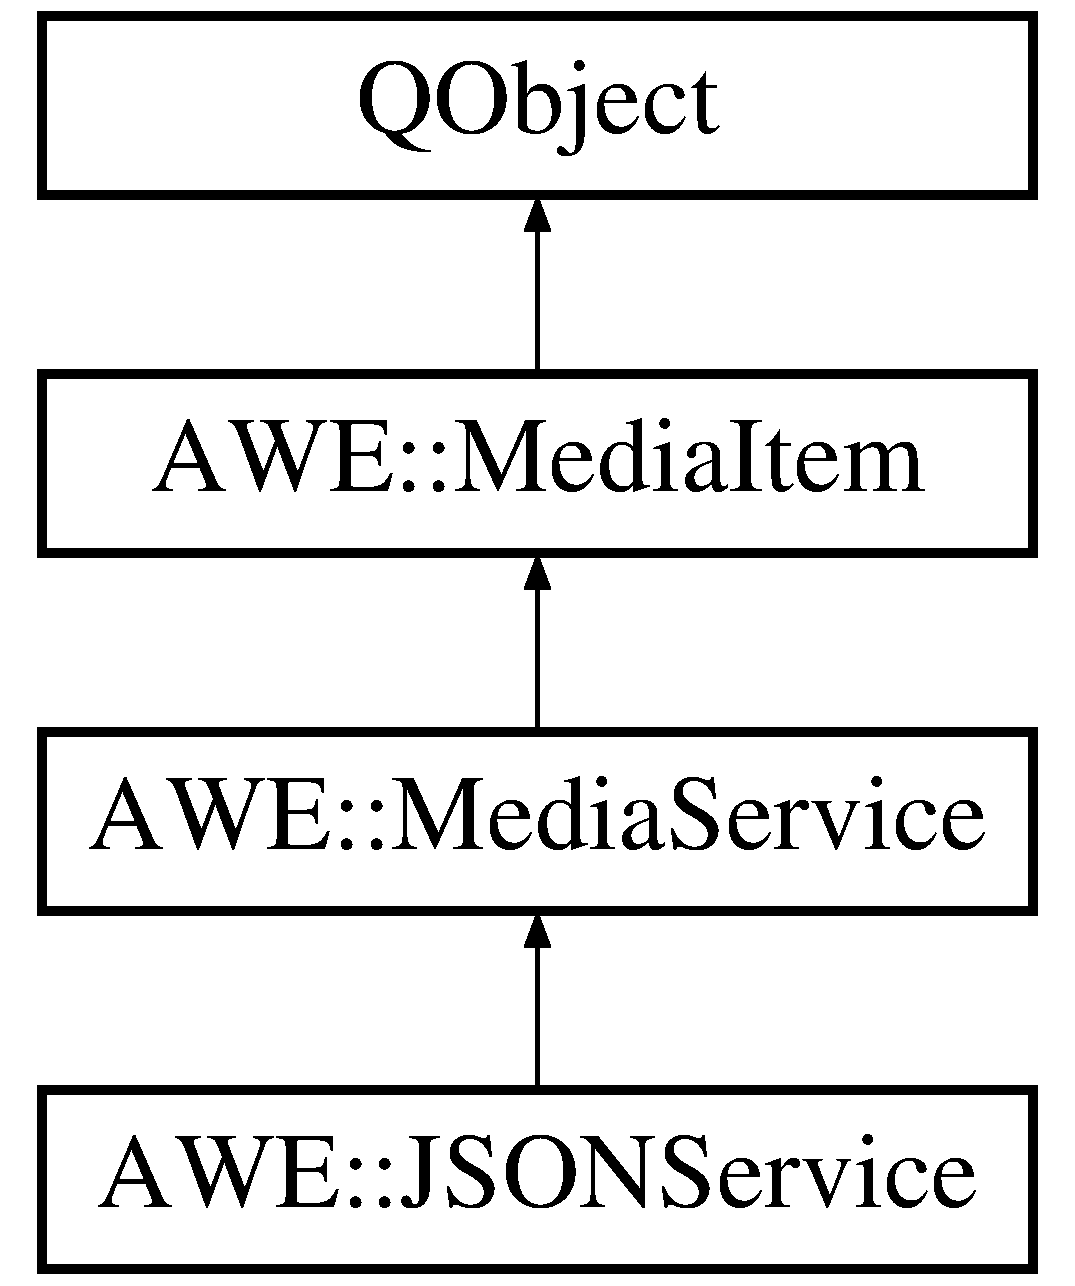
\includegraphics[height=3.000000cm]{class_a_w_e_1_1_media_service}
\end{center}
\end{figure}
\subsection*{Public Member Functions}
\begin{DoxyCompactItemize}
\item 
\hyperlink{class_a_w_e_1_1_media_service_ac843939cc99358391e249e5fbaa4e318}{Media\-Service} (const Q\-Dir \&file)
\begin{DoxyCompactList}\small\item\em Construct from thie given J\-S\-O\-N file. \end{DoxyCompactList}\item 
virtual int \hyperlink{class_a_w_e_1_1_media_service_ad13c100468482ce42880941bbeca4623}{open} ()=0
\begin{DoxyCompactList}\small\item\em Open the media service. \end{DoxyCompactList}\item 
virtual Item\-Type \hyperlink{class_a_w_e_1_1_media_service_a680d2f9fd50b27cb7156c3a5777dee12}{get\-Item\-Type} () const 
\begin{DoxyCompactList}\small\item\em Get the type of this item. \end{DoxyCompactList}\end{DoxyCompactItemize}
\subsection*{Additional Inherited Members}


\subsection{Detailed Description}
A media service, which is basically an application with its own media browser. 

\subsection{Constructor \& Destructor Documentation}
\hypertarget{class_a_w_e_1_1_media_service_ac843939cc99358391e249e5fbaa4e318}{\index{A\-W\-E\-::\-Media\-Service@{A\-W\-E\-::\-Media\-Service}!Media\-Service@{Media\-Service}}
\index{Media\-Service@{Media\-Service}!AWE::MediaService@{A\-W\-E\-::\-Media\-Service}}
\subsubsection[{Media\-Service}]{\setlength{\rightskip}{0pt plus 5cm}Media\-Service\-::\-Media\-Service (
\begin{DoxyParamCaption}
\item[{const Q\-Dir \&}]{file}
\end{DoxyParamCaption}
)}}\label{class_a_w_e_1_1_media_service_ac843939cc99358391e249e5fbaa4e318}


Construct from thie given J\-S\-O\-N file. 


\begin{DoxyParams}{Parameters}
{\em file} & The J\-S\-O\-N file for this service. \\
\hline
\end{DoxyParams}


\subsection{Member Function Documentation}
\hypertarget{class_a_w_e_1_1_media_service_a680d2f9fd50b27cb7156c3a5777dee12}{\index{A\-W\-E\-::\-Media\-Service@{A\-W\-E\-::\-Media\-Service}!get\-Item\-Type@{get\-Item\-Type}}
\index{get\-Item\-Type@{get\-Item\-Type}!AWE::MediaService@{A\-W\-E\-::\-Media\-Service}}
\subsubsection[{get\-Item\-Type}]{\setlength{\rightskip}{0pt plus 5cm}Item\-Type Media\-Service\-::get\-Item\-Type (
\begin{DoxyParamCaption}
{}
\end{DoxyParamCaption}
) const\hspace{0.3cm}{\ttfamily [virtual]}}}\label{class_a_w_e_1_1_media_service_a680d2f9fd50b27cb7156c3a5777dee12}


Get the type of this item. 

\begin{DoxyReturn}{Returns}
S\-E\-R\-V\-I\-C\-E\-\_\-\-T\-Y\-P\-E 
\end{DoxyReturn}


Implements \hyperlink{class_a_w_e_1_1_media_item_ad7a7ef28069986fad8b2be060fef6e48}{A\-W\-E\-::\-Media\-Item}.

\hypertarget{class_a_w_e_1_1_media_service_ad13c100468482ce42880941bbeca4623}{\index{A\-W\-E\-::\-Media\-Service@{A\-W\-E\-::\-Media\-Service}!open@{open}}
\index{open@{open}!AWE::MediaService@{A\-W\-E\-::\-Media\-Service}}
\subsubsection[{open}]{\setlength{\rightskip}{0pt plus 5cm}virtual int A\-W\-E\-::\-Media\-Service\-::open (
\begin{DoxyParamCaption}
{}
\end{DoxyParamCaption}
)\hspace{0.3cm}{\ttfamily [pure virtual]}}}\label{class_a_w_e_1_1_media_service_ad13c100468482ce42880941bbeca4623}


Open the media service. 

\begin{DoxyReturn}{Returns}
The exit code of the application. 
\end{DoxyReturn}


Implemented in \hyperlink{class_a_w_e_1_1_j_s_o_n_service_a19bbb59a75a05ad22d768d73febeeeda}{A\-W\-E\-::\-J\-S\-O\-N\-Service}.



The documentation for this class was generated from the following files\-:\begin{DoxyCompactItemize}
\item 
/\-Users/\-Alex/github/\-A\-W\-E\-Media\-Center/\-Code/items/A\-W\-E\-Media\-Service.\-h\item 
/\-Users/\-Alex/github/\-A\-W\-E\-Media\-Center/\-Code/items/A\-W\-E\-Media\-Service.\-cpp\end{DoxyCompactItemize}

\hypertarget{class_a_w_e_1_1_metadata_scraper}{\section{A\-W\-E\-:\-:Metadata\-Scraper Class Reference}
\label{class_a_w_e_1_1_metadata_scraper}\index{A\-W\-E\-::\-Metadata\-Scraper@{A\-W\-E\-::\-Metadata\-Scraper}}
}


Defines the general interface for a metadata scraper.  




{\ttfamily \#include $<$A\-W\-E\-Metadata\-Scraper.\-h$>$}

Inheritance diagram for A\-W\-E\-:\-:Metadata\-Scraper\-:\begin{figure}[H]
\begin{center}
\leavevmode
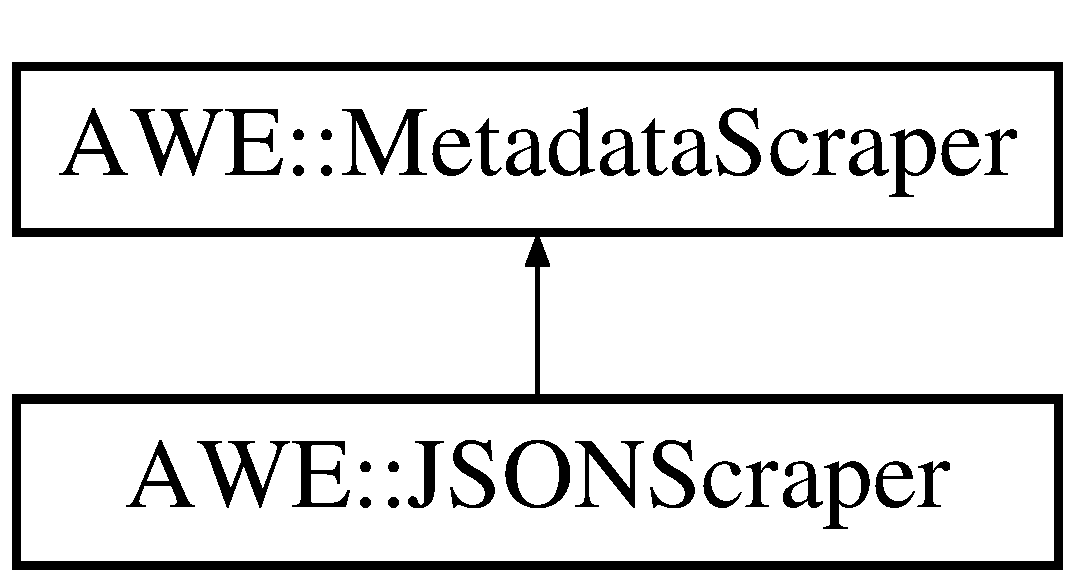
\includegraphics[height=2.000000cm]{class_a_w_e_1_1_metadata_scraper}
\end{center}
\end{figure}
\subsection*{Public Member Functions}
\begin{DoxyCompactItemize}
\item 
\hypertarget{class_a_w_e_1_1_metadata_scraper_a0a7ae0178e838b07bbd960be7c9e7dac}{virtual \hyperlink{class_a_w_e_1_1_metadata_scraper_a0a7ae0178e838b07bbd960be7c9e7dac}{$\sim$\-Metadata\-Scraper} ()}\label{class_a_w_e_1_1_metadata_scraper_a0a7ae0178e838b07bbd960be7c9e7dac}

\begin{DoxyCompactList}\small\item\em Deconstructor. \end{DoxyCompactList}\item 
virtual bool \hyperlink{class_a_w_e_1_1_metadata_scraper_a92f9039770add633140b825bf41bc30a}{prepare} (\hyperlink{class_a_w_e_1_1_global_settings}{Global\-Settings} $\ast$settings)=0
\begin{DoxyCompactList}\small\item\em Prepares the scraper. \end{DoxyCompactList}\item 
virtual bool \hyperlink{class_a_w_e_1_1_metadata_scraper_a509832b172ce67e5e9788134016481b3}{scrape\-Data\-For\-File} (\hyperlink{class_a_w_e_1_1_media_file}{Media\-File} $\ast$file, bool ask\-User, bool import)=0
\begin{DoxyCompactList}\small\item\em Retrieves metadata for a media file. \end{DoxyCompactList}\item 
virtual void \hyperlink{class_a_w_e_1_1_metadata_scraper_a9a90e9974be775dff73c004ada209cb0}{deactivate} ()=0
\begin{DoxyCompactList}\small\item\em Destroys any used-\/up dynamic memory. \end{DoxyCompactList}\item 
virtual bool \hyperlink{class_a_w_e_1_1_metadata_scraper_a06f9da8e43ac52378ec15fc849e42eb8}{is\-Valid} ()=0
\begin{DoxyCompactList}\small\item\em Determines if this is scraper can be used. \end{DoxyCompactList}\item 
virtual const std\-::string \& \hyperlink{class_a_w_e_1_1_metadata_scraper_a375745d101342f062a1a3eb89a63ec6b}{get\-Name} ()=0
\begin{DoxyCompactList}\small\item\em Gets the name of the scraper. \end{DoxyCompactList}\item 
virtual const std\-::string \& \hyperlink{class_a_w_e_1_1_metadata_scraper_a02549221a803b624300ea6994be1b1a2}{get\-Type} ()=0
\begin{DoxyCompactList}\small\item\em Gets the media type for this scraper. \end{DoxyCompactList}\end{DoxyCompactItemize}


\subsection{Detailed Description}
Defines the general interface for a metadata scraper. 

Metadata scrapers must take in the path to a media file and use that path to collect icons, fanart images, and other details about the media item.

In order to scrape for metadata, A\-W\-E\-M\-C does the following\-:
\begin{DoxyItemize}
\item Prepare the scraper by calling {\ttfamily \hyperlink{class_a_w_e_1_1_metadata_scraper_a92f9039770add633140b825bf41bc30a}{prepare()}}.
\item Scrape for metadata using {\ttfamily \hyperlink{class_a_w_e_1_1_metadata_scraper_a509832b172ce67e5e9788134016481b3}{scrape\-Data\-For\-File()}}.
\item Deactivate the scraper by calling {\ttfamily \hyperlink{class_a_w_e_1_1_metadata_scraper_a9a90e9974be775dff73c004ada209cb0}{deactivate()}}.
\end{DoxyItemize}

{\ttfamily \hyperlink{class_a_w_e_1_1_metadata_scraper}{Metadata\-Scraper}} implementations should be largely immutable, at least as seen by the functions outside of the class. The only place internal changes should be made is during the scraping of a file with temporary instance variables. 

\subsection{Member Function Documentation}
\hypertarget{class_a_w_e_1_1_metadata_scraper_a9a90e9974be775dff73c004ada209cb0}{\index{A\-W\-E\-::\-Metadata\-Scraper@{A\-W\-E\-::\-Metadata\-Scraper}!deactivate@{deactivate}}
\index{deactivate@{deactivate}!AWE::MetadataScraper@{A\-W\-E\-::\-Metadata\-Scraper}}
\subsubsection[{deactivate}]{\setlength{\rightskip}{0pt plus 5cm}virtual void A\-W\-E\-::\-Metadata\-Scraper\-::deactivate (
\begin{DoxyParamCaption}
{}
\end{DoxyParamCaption}
)\hspace{0.3cm}{\ttfamily [pure virtual]}}}\label{class_a_w_e_1_1_metadata_scraper_a9a90e9974be775dff73c004ada209cb0}


Destroys any used-\/up dynamic memory. 

This helps with memory management. If you rely on large objects to scrape for metadata, this is where you should {\ttfamily delete} them. 

Implemented in \hyperlink{class_a_w_e_1_1_j_s_o_n_scraper_a0d1a05a4c7273ff1063518592d68501a}{A\-W\-E\-::\-J\-S\-O\-N\-Scraper}.

\hypertarget{class_a_w_e_1_1_metadata_scraper_a375745d101342f062a1a3eb89a63ec6b}{\index{A\-W\-E\-::\-Metadata\-Scraper@{A\-W\-E\-::\-Metadata\-Scraper}!get\-Name@{get\-Name}}
\index{get\-Name@{get\-Name}!AWE::MetadataScraper@{A\-W\-E\-::\-Metadata\-Scraper}}
\subsubsection[{get\-Name}]{\setlength{\rightskip}{0pt plus 5cm}virtual const std\-::string\& A\-W\-E\-::\-Metadata\-Scraper\-::get\-Name (
\begin{DoxyParamCaption}
{}
\end{DoxyParamCaption}
)\hspace{0.3cm}{\ttfamily [pure virtual]}}}\label{class_a_w_e_1_1_metadata_scraper_a375745d101342f062a1a3eb89a63ec6b}


Gets the name of the scraper. 

\begin{DoxyReturn}{Returns}
The name of the scraper. 
\end{DoxyReturn}


Implemented in \hyperlink{class_a_w_e_1_1_j_s_o_n_scraper_a77c2ed4ece4a88876f6381b97d6c5a93}{A\-W\-E\-::\-J\-S\-O\-N\-Scraper}.

\hypertarget{class_a_w_e_1_1_metadata_scraper_a02549221a803b624300ea6994be1b1a2}{\index{A\-W\-E\-::\-Metadata\-Scraper@{A\-W\-E\-::\-Metadata\-Scraper}!get\-Type@{get\-Type}}
\index{get\-Type@{get\-Type}!AWE::MetadataScraper@{A\-W\-E\-::\-Metadata\-Scraper}}
\subsubsection[{get\-Type}]{\setlength{\rightskip}{0pt plus 5cm}virtual const std\-::string\& A\-W\-E\-::\-Metadata\-Scraper\-::get\-Type (
\begin{DoxyParamCaption}
{}
\end{DoxyParamCaption}
)\hspace{0.3cm}{\ttfamily [pure virtual]}}}\label{class_a_w_e_1_1_metadata_scraper_a02549221a803b624300ea6994be1b1a2}


Gets the media type for this scraper. 

\begin{DoxyReturn}{Returns}
The media type name for the scraper. 
\end{DoxyReturn}


Implemented in \hyperlink{class_a_w_e_1_1_j_s_o_n_scraper_a5b540056aa7ddf4e343220b0a54a0279}{A\-W\-E\-::\-J\-S\-O\-N\-Scraper}.

\hypertarget{class_a_w_e_1_1_metadata_scraper_a06f9da8e43ac52378ec15fc849e42eb8}{\index{A\-W\-E\-::\-Metadata\-Scraper@{A\-W\-E\-::\-Metadata\-Scraper}!is\-Valid@{is\-Valid}}
\index{is\-Valid@{is\-Valid}!AWE::MetadataScraper@{A\-W\-E\-::\-Metadata\-Scraper}}
\subsubsection[{is\-Valid}]{\setlength{\rightskip}{0pt plus 5cm}virtual bool A\-W\-E\-::\-Metadata\-Scraper\-::is\-Valid (
\begin{DoxyParamCaption}
{}
\end{DoxyParamCaption}
)\hspace{0.3cm}{\ttfamily [pure virtual]}}}\label{class_a_w_e_1_1_metadata_scraper_a06f9da8e43ac52378ec15fc849e42eb8}


Determines if this is scraper can be used. 

\begin{DoxyReturn}{Returns}
{\ttfamily true} if this scraper can be used successfully, {\ttfamily false} otherwise. 
\end{DoxyReturn}


Implemented in \hyperlink{class_a_w_e_1_1_j_s_o_n_scraper_abb4ca61ee617b473198a635c6f3ac57d}{A\-W\-E\-::\-J\-S\-O\-N\-Scraper}.

\hypertarget{class_a_w_e_1_1_metadata_scraper_a92f9039770add633140b825bf41bc30a}{\index{A\-W\-E\-::\-Metadata\-Scraper@{A\-W\-E\-::\-Metadata\-Scraper}!prepare@{prepare}}
\index{prepare@{prepare}!AWE::MetadataScraper@{A\-W\-E\-::\-Metadata\-Scraper}}
\subsubsection[{prepare}]{\setlength{\rightskip}{0pt plus 5cm}virtual bool A\-W\-E\-::\-Metadata\-Scraper\-::prepare (
\begin{DoxyParamCaption}
\item[{{\bf Global\-Settings} $\ast$}]{settings}
\end{DoxyParamCaption}
)\hspace{0.3cm}{\ttfamily [pure virtual]}}}\label{class_a_w_e_1_1_metadata_scraper_a92f9039770add633140b825bf41bc30a}


Prepares the scraper. 

This helps with memory management. If you rely on large objects to scrape for metadata, this is where you should construct them.


\begin{DoxyParams}[1]{Parameters}
\mbox{\tt in}  & {\em settings} & The ../settings/\-R\-E\-A\-D\-M\-E.md \char`\"{}global settings of A\-W\-E\-M\-C\char`\"{}, so that your scraper can be customized.\\
\hline
\end{DoxyParams}
\begin{DoxyReturn}{Returns}
{\ttfamily true} if the scraper was able to prepare itself, {\ttfamily false} if an error occured and scraping should be aborted. 
\end{DoxyReturn}


Implemented in \hyperlink{class_a_w_e_1_1_j_s_o_n_scraper_a1b12fde072ef979911fcca4191c3c2a7}{A\-W\-E\-::\-J\-S\-O\-N\-Scraper}.

\hypertarget{class_a_w_e_1_1_metadata_scraper_a509832b172ce67e5e9788134016481b3}{\index{A\-W\-E\-::\-Metadata\-Scraper@{A\-W\-E\-::\-Metadata\-Scraper}!scrape\-Data\-For\-File@{scrape\-Data\-For\-File}}
\index{scrape\-Data\-For\-File@{scrape\-Data\-For\-File}!AWE::MetadataScraper@{A\-W\-E\-::\-Metadata\-Scraper}}
\subsubsection[{scrape\-Data\-For\-File}]{\setlength{\rightskip}{0pt plus 5cm}virtual bool A\-W\-E\-::\-Metadata\-Scraper\-::scrape\-Data\-For\-File (
\begin{DoxyParamCaption}
\item[{{\bf Media\-File} $\ast$}]{file, }
\item[{bool}]{ask\-User, }
\item[{bool}]{import}
\end{DoxyParamCaption}
)\hspace{0.3cm}{\ttfamily [pure virtual]}}}\label{class_a_w_e_1_1_metadata_scraper_a509832b172ce67e5e9788134016481b3}


Retrieves metadata for a media file. 

You must write the metadata to {\ttfamily file}.

To construct your J\-S\-O\-N file, you should use \href{http://jsoncpp.sourceforge.net}{\tt jsoncpp}.

{\ttfamily ask\-User} tells your scraper if the user wants to be given a list of choices for certain things. You should N\-O\-T ask the user for everything if {\ttfamily ask\-User} is true; only basic things like, \char`\"{}\-Which icon do you want to use?\char`\"{}

{\ttfamily import} specifies if the files you get should be copied into A\-W\-E\-M\-C's folders. Do N\-O\-T copy the media file.


\begin{DoxyParams}[1]{Parameters}
\mbox{\tt in,out}  & {\em file} & The media file to get metadata for. \\
\hline
\mbox{\tt in}  & {\em ask\-User} & {\ttfamily true} if the user wants to be given choices, {\ttfamily false} otherwise. \\
\hline
\mbox{\tt in}  & {\em import} & {\ttfamily true} if the user wants to import metadata files, {\ttfamily false} otherwise.\\
\hline
\end{DoxyParams}
\begin{DoxyReturn}{Returns}
{\ttfamily true} if the scraper was able to get the metadata, {\ttfamily false} if it was not. 
\end{DoxyReturn}


Implemented in \hyperlink{class_a_w_e_1_1_j_s_o_n_scraper_afbed287c0fcae8d797552c711854b4e9}{A\-W\-E\-::\-J\-S\-O\-N\-Scraper}.



The documentation for this class was generated from the following file\-:\begin{DoxyCompactItemize}
\item 
/\-Users/\-Alex/github/\-A\-W\-E\-Media\-Center/\-Code/scraper/A\-W\-E\-Metadata\-Scraper.\-h\end{DoxyCompactItemize}

\hypertarget{class_json_1_1_path}{\section{Json\-:\-:Path Class Reference}
\label{class_json_1_1_path}\index{Json\-::\-Path@{Json\-::\-Path}}
}


Experimental and untested\-: represents a \char`\"{}path\char`\"{} to access a node.  




{\ttfamily \#include $<$json.\-h$>$}

\subsection*{Public Member Functions}
\begin{DoxyCompactItemize}
\item 
\hypertarget{class_json_1_1_path_aaa37a99650e770d0cd680bf53585ec99}{{\bfseries Path} (const std\-::string \&path, const \hyperlink{class_json_1_1_path_argument}{Path\-Argument} \&a1=\hyperlink{class_json_1_1_path_argument}{Path\-Argument}(), const \hyperlink{class_json_1_1_path_argument}{Path\-Argument} \&a2=\hyperlink{class_json_1_1_path_argument}{Path\-Argument}(), const \hyperlink{class_json_1_1_path_argument}{Path\-Argument} \&a3=\hyperlink{class_json_1_1_path_argument}{Path\-Argument}(), const \hyperlink{class_json_1_1_path_argument}{Path\-Argument} \&a4=\hyperlink{class_json_1_1_path_argument}{Path\-Argument}(), const \hyperlink{class_json_1_1_path_argument}{Path\-Argument} \&a5=\hyperlink{class_json_1_1_path_argument}{Path\-Argument}())}\label{class_json_1_1_path_aaa37a99650e770d0cd680bf53585ec99}

\item 
\hypertarget{class_json_1_1_path_ae1d05fa985a6ee3c57f2b8ed186b5982}{const \hyperlink{class_json_1_1_value}{Value} \& {\bfseries resolve} (const \hyperlink{class_json_1_1_value}{Value} \&root) const }\label{class_json_1_1_path_ae1d05fa985a6ee3c57f2b8ed186b5982}

\item 
\hypertarget{class_json_1_1_path_a33d1749770a4cf74e9a3de419bc7febe}{\hyperlink{class_json_1_1_value}{Value} {\bfseries resolve} (const \hyperlink{class_json_1_1_value}{Value} \&root, const \hyperlink{class_json_1_1_value}{Value} \&default\-Value) const }\label{class_json_1_1_path_a33d1749770a4cf74e9a3de419bc7febe}

\item 
\hypertarget{class_json_1_1_path_a5289901fc58ad1fdca1de7fb5a0b620c}{\hyperlink{class_json_1_1_value}{Value} \& \hyperlink{class_json_1_1_path_a5289901fc58ad1fdca1de7fb5a0b620c}{make} (\hyperlink{class_json_1_1_value}{Value} \&root) const }\label{class_json_1_1_path_a5289901fc58ad1fdca1de7fb5a0b620c}

\begin{DoxyCompactList}\small\item\em Creates the \char`\"{}path\char`\"{} to access the specified node and returns a reference on the node. \end{DoxyCompactList}\end{DoxyCompactItemize}
\subsection*{Private Types}
\begin{DoxyCompactItemize}
\item 
\hypertarget{class_json_1_1_path_a763349989466ac275fad176708378f95}{typedef std\-::vector$<$ const \\*
\hyperlink{class_json_1_1_path_argument}{Path\-Argument} $\ast$ $>$ {\bfseries In\-Args}}\label{class_json_1_1_path_a763349989466ac275fad176708378f95}

\item 
\hypertarget{class_json_1_1_path_a27d96232d034d7a78286468676f9cb3e}{typedef std\-::vector$<$ \hyperlink{class_json_1_1_path_argument}{Path\-Argument} $>$ {\bfseries Args}}\label{class_json_1_1_path_a27d96232d034d7a78286468676f9cb3e}

\end{DoxyCompactItemize}
\subsection*{Private Member Functions}
\begin{DoxyCompactItemize}
\item 
\hypertarget{class_json_1_1_path_a874e5339f8059ebeef049721f8897277}{void {\bfseries make\-Path} (const std\-::string \&path, const In\-Args \&in)}\label{class_json_1_1_path_a874e5339f8059ebeef049721f8897277}

\item 
\hypertarget{class_json_1_1_path_af4d2ab3a6f09b69bab3d3e9fcdf13328}{void {\bfseries add\-Path\-In\-Arg} (const std\-::string \&path, const In\-Args \&in, In\-Args\-::const\-\_\-iterator \&it\-In\-Arg, Path\-Argument\-::\-Kind kind)}\label{class_json_1_1_path_af4d2ab3a6f09b69bab3d3e9fcdf13328}

\item 
\hypertarget{class_json_1_1_path_a3729e6d3682338b2cfad2c10d4746f53}{void {\bfseries invalid\-Path} (const std\-::string \&path, int location)}\label{class_json_1_1_path_a3729e6d3682338b2cfad2c10d4746f53}

\end{DoxyCompactItemize}
\subsection*{Private Attributes}
\begin{DoxyCompactItemize}
\item 
\hypertarget{class_json_1_1_path_af33d0de7ee9f99d3e361bdf504dc2bc7}{Args {\bfseries args\-\_\-}}\label{class_json_1_1_path_af33d0de7ee9f99d3e361bdf504dc2bc7}

\end{DoxyCompactItemize}


\subsection{Detailed Description}
Experimental and untested\-: represents a \char`\"{}path\char`\"{} to access a node. 

Syntax\-:
\begin{DoxyItemize}
\item \char`\"{}.\char`\"{} =$>$ root node
\item \char`\"{}.\mbox{[}n\mbox{]}\char`\"{} =$>$ elements at index 'n' of root node (an array value)
\item \char`\"{}.\-name\char`\"{} =$>$ member named 'name' of root node (an object value)
\item \char`\"{}.\-name1.\-name2.\-name3\char`\"{}
\item \char`\"{}.\mbox{[}0\mbox{]}\mbox{[}1\mbox{]}\mbox{[}2\mbox{]}.\-name1\mbox{[}3\mbox{]}\char`\"{}
\item \char`\"{}.\%\char`\"{} =$>$ member name is provided as parameter
\item \char`\"{}.\mbox{[}\%\mbox{]}\char`\"{} =$>$ index is provied as parameter 
\end{DoxyItemize}

The documentation for this class was generated from the following files\-:\begin{DoxyCompactItemize}
\item 
/\-Users/\-Alex/github/\-A\-W\-E\-Media\-Center/\-Code/libs/json/json.\-h\item 
/\-Users/\-Alex/github/\-A\-W\-E\-Media\-Center/\-Code/libs/json/jsoncpp.\-cpp\end{DoxyCompactItemize}

\hypertarget{class_json_1_1_path_argument}{\section{Json\-:\-:Path\-Argument Class Reference}
\label{class_json_1_1_path_argument}\index{Json\-::\-Path\-Argument@{Json\-::\-Path\-Argument}}
}


Experimental and untested\-: represents an element of the \char`\"{}path\char`\"{} to access a node.  




{\ttfamily \#include $<$json.\-h$>$}

\subsection*{Public Member Functions}
\begin{DoxyCompactItemize}
\item 
\hypertarget{class_json_1_1_path_argument_a53c5b27143b161301b95fd544c139ecf}{{\bfseries Path\-Argument} (Array\-Index index)}\label{class_json_1_1_path_argument_a53c5b27143b161301b95fd544c139ecf}

\item 
\hypertarget{class_json_1_1_path_argument_a9690417a8a40e6e49f2acdf6c9281345}{{\bfseries Path\-Argument} (const char $\ast$key)}\label{class_json_1_1_path_argument_a9690417a8a40e6e49f2acdf6c9281345}

\item 
\hypertarget{class_json_1_1_path_argument_a08f872cfee4fc600f7fa3bcaaff0d41c}{{\bfseries Path\-Argument} (const std\-::string \&key)}\label{class_json_1_1_path_argument_a08f872cfee4fc600f7fa3bcaaff0d41c}

\end{DoxyCompactItemize}
\subsection*{Friends}
\begin{DoxyCompactItemize}
\item 
\hypertarget{class_json_1_1_path_argument_a4877239a6b7f09fbf5a61ca68a49d74c}{class {\bfseries Path}}\label{class_json_1_1_path_argument_a4877239a6b7f09fbf5a61ca68a49d74c}

\end{DoxyCompactItemize}


\subsection{Detailed Description}
Experimental and untested\-: represents an element of the \char`\"{}path\char`\"{} to access a node. 

The documentation for this class was generated from the following files\-:\begin{DoxyCompactItemize}
\item 
/\-Users/\-Alex/github/\-A\-W\-E\-Media\-Center/\-Code/libs/json/json.\-h\item 
/\-Users/\-Alex/github/\-A\-W\-E\-Media\-Center/\-Code/libs/json/jsoncpp.\-cpp\end{DoxyCompactItemize}

\hypertarget{class_json_1_1_reader}{\section{Json\-:\-:Reader Class Reference}
\label{class_json_1_1_reader}\index{Json\-::\-Reader@{Json\-::\-Reader}}
}


Unserialize a \href{http://www.json.org}{\tt J\-S\-O\-N} document into a \hyperlink{class_json_1_1_value}{Value}.  




{\ttfamily \#include $<$json.\-h$>$}

\subsection*{Classes}
\begin{DoxyCompactItemize}
\item 
class \hyperlink{class_json_1_1_reader_1_1_error_info}{Error\-Info}
\item 
class \hyperlink{class_json_1_1_reader_1_1_token}{Token}
\end{DoxyCompactItemize}
\subsection*{Public Types}
\begin{DoxyCompactItemize}
\item 
\hypertarget{class_json_1_1_reader_a3eec9118f3e9a672ba8348c3a79d0f45}{typedef char {\bfseries Char}}\label{class_json_1_1_reader_a3eec9118f3e9a672ba8348c3a79d0f45}

\item 
\hypertarget{class_json_1_1_reader_a46795b5b272bf79a7730e406cb96375a}{typedef const Char $\ast$ {\bfseries Location}}\label{class_json_1_1_reader_a46795b5b272bf79a7730e406cb96375a}

\end{DoxyCompactItemize}
\subsection*{Public Member Functions}
\begin{DoxyCompactItemize}
\item 
\hypertarget{class_json_1_1_reader_a0b3c4e24c8393354bab57a6ba3ffc27f}{\hyperlink{class_json_1_1_reader_a0b3c4e24c8393354bab57a6ba3ffc27f}{Reader} ()}\label{class_json_1_1_reader_a0b3c4e24c8393354bab57a6ba3ffc27f}

\begin{DoxyCompactList}\small\item\em Constructs a \hyperlink{class_json_1_1_reader}{Reader} allowing all features for parsing. \end{DoxyCompactList}\item 
\hypertarget{class_json_1_1_reader_a45f17831118337309180313e93ac33f8}{\hyperlink{class_json_1_1_reader_a45f17831118337309180313e93ac33f8}{Reader} (const \hyperlink{class_json_1_1_features}{Features} \&features)}\label{class_json_1_1_reader_a45f17831118337309180313e93ac33f8}

\begin{DoxyCompactList}\small\item\em Constructs a \hyperlink{class_json_1_1_reader}{Reader} allowing the specified feature set for parsing. \end{DoxyCompactList}\item 
bool \hyperlink{class_json_1_1_reader_af1da6c976ad1e96c742804c3853eef94}{parse} (const std\-::string \&document, \hyperlink{class_json_1_1_value}{Value} \&root, bool collect\-Comments=true)
\begin{DoxyCompactList}\small\item\em Read a \hyperlink{class_json_1_1_value}{Value} from a \href{http://www.json.org}{\tt J\-S\-O\-N} document. \end{DoxyCompactList}\item 
bool \hyperlink{class_json_1_1_reader_ac71ef2b64c7c27b062052e692af3fb32}{parse} (const char $\ast$begin\-Doc, const char $\ast$end\-Doc, \hyperlink{class_json_1_1_value}{Value} \&root, bool collect\-Comments=true)
\begin{DoxyCompactList}\small\item\em Read a \hyperlink{class_json_1_1_value}{Value} from a \href{http://www.json.org}{\tt J\-S\-O\-N} document. \end{DoxyCompactList}\item 
bool \hyperlink{class_json_1_1_reader_a8d0347e6b47343e4bc68be7ecdb9c4e9}{parse} (std\-::istream \&is, \hyperlink{class_json_1_1_value}{Value} \&root, bool collect\-Comments=true)
\begin{DoxyCompactList}\small\item\em Parse from input stream. \end{DoxyCompactList}\item 
std\-::string \hyperlink{class_json_1_1_reader_afa4a59e962d23c4d1c38b433fc95eefa}{get\-Formated\-Error\-Messages} () const 
\begin{DoxyCompactList}\small\item\em Returns a user friendly string that list errors in the parsed document. \end{DoxyCompactList}\item 
std\-::string \hyperlink{class_json_1_1_reader_a95ab50aa789132e9dee0fc1475c85acf}{get\-Formatted\-Error\-Messages} () const 
\begin{DoxyCompactList}\small\item\em Returns a user friendly string that list errors in the parsed document. \end{DoxyCompactList}\end{DoxyCompactItemize}
\subsection*{Private Types}
\begin{DoxyCompactItemize}
\item 
enum {\bfseries Token\-Type} \{ \\*
{\bfseries token\-End\-Of\-Stream} = 0, 
{\bfseries token\-Object\-Begin}, 
{\bfseries token\-Object\-End}, 
{\bfseries token\-Array\-Begin}, 
\\*
{\bfseries token\-Array\-End}, 
{\bfseries token\-String}, 
{\bfseries token\-Number}, 
{\bfseries token\-True}, 
\\*
{\bfseries token\-False}, 
{\bfseries token\-Null}, 
{\bfseries token\-Array\-Separator}, 
{\bfseries token\-Member\-Separator}, 
\\*
{\bfseries token\-Comment}, 
{\bfseries token\-Error}
 \}
\item 
\hypertarget{class_json_1_1_reader_aae51e8f5bab3f067261c842a3ef858e5}{typedef std\-::deque$<$ \hyperlink{class_json_1_1_reader_1_1_error_info}{Error\-Info} $>$ {\bfseries Errors}}\label{class_json_1_1_reader_aae51e8f5bab3f067261c842a3ef858e5}

\item 
\hypertarget{class_json_1_1_reader_ad98d0ea4f3576ea83947c1b2b7b2f261}{typedef std\-::stack$<$ \hyperlink{class_json_1_1_value}{Value} $\ast$ $>$ {\bfseries Nodes}}\label{class_json_1_1_reader_ad98d0ea4f3576ea83947c1b2b7b2f261}

\end{DoxyCompactItemize}
\subsection*{Private Member Functions}
\begin{DoxyCompactItemize}
\item 
\hypertarget{class_json_1_1_reader_a442d779d60825634625040eed83eadc5}{bool {\bfseries expect\-Token} (Token\-Type type, \hyperlink{class_json_1_1_reader_1_1_token}{Token} \&token, const char $\ast$message)}\label{class_json_1_1_reader_a442d779d60825634625040eed83eadc5}

\item 
\hypertarget{class_json_1_1_reader_a7cb0631963cc0fd4ff6ed0f570976864}{bool {\bfseries read\-Token} (\hyperlink{class_json_1_1_reader_1_1_token}{Token} \&token)}\label{class_json_1_1_reader_a7cb0631963cc0fd4ff6ed0f570976864}

\item 
\hypertarget{class_json_1_1_reader_a40d0f69d15aeb2d52ff78d794f5ab8b2}{void {\bfseries skip\-Spaces} ()}\label{class_json_1_1_reader_a40d0f69d15aeb2d52ff78d794f5ab8b2}

\item 
\hypertarget{class_json_1_1_reader_a3e5a7bc6b7b53f2ca8cb9da42f8ffb21}{bool {\bfseries match} (Location pattern, int pattern\-Length)}\label{class_json_1_1_reader_a3e5a7bc6b7b53f2ca8cb9da42f8ffb21}

\item 
\hypertarget{class_json_1_1_reader_ad2690e860a1b3332c5401fb0850ba065}{bool {\bfseries read\-Comment} ()}\label{class_json_1_1_reader_ad2690e860a1b3332c5401fb0850ba065}

\item 
\hypertarget{class_json_1_1_reader_ae0ffe796abdc3c5851589ee500e28c79}{bool {\bfseries read\-C\-Style\-Comment} ()}\label{class_json_1_1_reader_ae0ffe796abdc3c5851589ee500e28c79}

\item 
\hypertarget{class_json_1_1_reader_a6716ef6290b0f469efaf8d379c357967}{bool {\bfseries read\-Cpp\-Style\-Comment} ()}\label{class_json_1_1_reader_a6716ef6290b0f469efaf8d379c357967}

\item 
\hypertarget{class_json_1_1_reader_a6328a0b1994e05118886f9fc9c608643}{bool {\bfseries read\-String} ()}\label{class_json_1_1_reader_a6328a0b1994e05118886f9fc9c608643}

\item 
\hypertarget{class_json_1_1_reader_afb31bfda6bb27d6453057a47655e8363}{void {\bfseries read\-Number} ()}\label{class_json_1_1_reader_afb31bfda6bb27d6453057a47655e8363}

\item 
\hypertarget{class_json_1_1_reader_a47e56844b803d41ec993a83fadf4495c}{bool {\bfseries read\-Value} ()}\label{class_json_1_1_reader_a47e56844b803d41ec993a83fadf4495c}

\item 
\hypertarget{class_json_1_1_reader_a0068eb3d8e86e91f0e4806f60da66b9c}{bool {\bfseries read\-Object} (\hyperlink{class_json_1_1_reader_1_1_token}{Token} \&token)}\label{class_json_1_1_reader_a0068eb3d8e86e91f0e4806f60da66b9c}

\item 
\hypertarget{class_json_1_1_reader_afd9a30c0af205c9f327613f486fae6b8}{bool {\bfseries read\-Array} (\hyperlink{class_json_1_1_reader_1_1_token}{Token} \&token)}\label{class_json_1_1_reader_afd9a30c0af205c9f327613f486fae6b8}

\item 
\hypertarget{class_json_1_1_reader_a442d1f23edf0f4350f5eeab3ee3f7d46}{bool {\bfseries decode\-Number} (\hyperlink{class_json_1_1_reader_1_1_token}{Token} \&token)}\label{class_json_1_1_reader_a442d1f23edf0f4350f5eeab3ee3f7d46}

\item 
\hypertarget{class_json_1_1_reader_aaf736937912f5c9b8d221e57f209e3e0}{bool {\bfseries decode\-String} (\hyperlink{class_json_1_1_reader_1_1_token}{Token} \&token)}\label{class_json_1_1_reader_aaf736937912f5c9b8d221e57f209e3e0}

\item 
\hypertarget{class_json_1_1_reader_a801253570f16e91519652078fb12b8e6}{bool {\bfseries decode\-String} (\hyperlink{class_json_1_1_reader_1_1_token}{Token} \&token, std\-::string \&decoded)}\label{class_json_1_1_reader_a801253570f16e91519652078fb12b8e6}

\item 
\hypertarget{class_json_1_1_reader_a2420bbb7fd6d5d3e7e2fea894dd8f70f}{bool {\bfseries decode\-Double} (\hyperlink{class_json_1_1_reader_1_1_token}{Token} \&token)}\label{class_json_1_1_reader_a2420bbb7fd6d5d3e7e2fea894dd8f70f}

\item 
\hypertarget{class_json_1_1_reader_a8fe24db3e9953aef3d637a56447e795c}{bool {\bfseries decode\-Unicode\-Code\-Point} (\hyperlink{class_json_1_1_reader_1_1_token}{Token} \&token, Location \&current, Location end, unsigned int \&unicode)}\label{class_json_1_1_reader_a8fe24db3e9953aef3d637a56447e795c}

\item 
\hypertarget{class_json_1_1_reader_a469cb6f55971d7c41fca2752a3aa5bf7}{bool {\bfseries decode\-Unicode\-Escape\-Sequence} (\hyperlink{class_json_1_1_reader_1_1_token}{Token} \&token, Location \&current, Location end, unsigned int \&unicode)}\label{class_json_1_1_reader_a469cb6f55971d7c41fca2752a3aa5bf7}

\item 
\hypertarget{class_json_1_1_reader_a04a3a13dbc609dfdf9e3c6723e37ff21}{bool {\bfseries add\-Error} (const std\-::string \&message, \hyperlink{class_json_1_1_reader_1_1_token}{Token} \&token, Location extra=0)}\label{class_json_1_1_reader_a04a3a13dbc609dfdf9e3c6723e37ff21}

\item 
\hypertarget{class_json_1_1_reader_a8d4ed03a43082c5ace81ba5b81425eaf}{bool {\bfseries recover\-From\-Error} (Token\-Type skip\-Until\-Token)}\label{class_json_1_1_reader_a8d4ed03a43082c5ace81ba5b81425eaf}

\item 
\hypertarget{class_json_1_1_reader_af47fb7564db6ac21faebaba8cebb41ce}{bool {\bfseries add\-Error\-And\-Recover} (const std\-::string \&message, \hyperlink{class_json_1_1_reader_1_1_token}{Token} \&token, Token\-Type skip\-Until\-Token)}\label{class_json_1_1_reader_af47fb7564db6ac21faebaba8cebb41ce}

\item 
\hypertarget{class_json_1_1_reader_ad922ea5a8ab333084edbb84827861fa3}{void {\bfseries skip\-Until\-Space} ()}\label{class_json_1_1_reader_ad922ea5a8ab333084edbb84827861fa3}

\item 
\hypertarget{class_json_1_1_reader_a85597f763fb0148a17359b6dfc6f7326}{\hyperlink{class_json_1_1_value}{Value} \& {\bfseries current\-Value} ()}\label{class_json_1_1_reader_a85597f763fb0148a17359b6dfc6f7326}

\item 
\hypertarget{class_json_1_1_reader_ab61eb61333cc9ec3afe785663a53ce90}{Char {\bfseries get\-Next\-Char} ()}\label{class_json_1_1_reader_ab61eb61333cc9ec3afe785663a53ce90}

\item 
\hypertarget{class_json_1_1_reader_a20b3023dc422726e2e4ebe41b8ba0515}{void {\bfseries get\-Location\-Line\-And\-Column} (Location location, int \&line, int \&column) const }\label{class_json_1_1_reader_a20b3023dc422726e2e4ebe41b8ba0515}

\item 
\hypertarget{class_json_1_1_reader_ac5b4b5a76d3224871519b0656393b35b}{std\-::string {\bfseries get\-Location\-Line\-And\-Column} (Location location) const }\label{class_json_1_1_reader_ac5b4b5a76d3224871519b0656393b35b}

\item 
\hypertarget{class_json_1_1_reader_aaea3bd62d12ffb6117a61476c0685049}{void {\bfseries add\-Comment} (Location begin, Location end, \hyperlink{namespace_json_a4fc417c23905b2ae9e2c47d197a45351}{Comment\-Placement} placement)}\label{class_json_1_1_reader_aaea3bd62d12ffb6117a61476c0685049}

\item 
\hypertarget{class_json_1_1_reader_a22e677ef400d8223f27e631b4cd4b821}{void {\bfseries skip\-Comment\-Tokens} (\hyperlink{class_json_1_1_reader_1_1_token}{Token} \&token)}\label{class_json_1_1_reader_a22e677ef400d8223f27e631b4cd4b821}

\end{DoxyCompactItemize}
\subsection*{Private Attributes}
\begin{DoxyCompactItemize}
\item 
\hypertarget{class_json_1_1_reader_ada3d2c47699dad662e6d156c8c78a6ac}{Nodes {\bfseries nodes\-\_\-}}\label{class_json_1_1_reader_ada3d2c47699dad662e6d156c8c78a6ac}

\item 
\hypertarget{class_json_1_1_reader_a1bbce45dc4df753bed60c129f4b5147c}{Errors {\bfseries errors\-\_\-}}\label{class_json_1_1_reader_a1bbce45dc4df753bed60c129f4b5147c}

\item 
\hypertarget{class_json_1_1_reader_afde4a4311ae30597da5b6060a8d60542}{std\-::string {\bfseries document\-\_\-}}\label{class_json_1_1_reader_afde4a4311ae30597da5b6060a8d60542}

\item 
\hypertarget{class_json_1_1_reader_a327166839022ea91f0a8290960a8af76}{Location {\bfseries begin\-\_\-}}\label{class_json_1_1_reader_a327166839022ea91f0a8290960a8af76}

\item 
\hypertarget{class_json_1_1_reader_a714793579cbf4ee7c5a7223d2c8d77c1}{Location {\bfseries end\-\_\-}}\label{class_json_1_1_reader_a714793579cbf4ee7c5a7223d2c8d77c1}

\item 
\hypertarget{class_json_1_1_reader_a2f2feb5201a26da7aa133d2f7434479b}{Location {\bfseries current\-\_\-}}\label{class_json_1_1_reader_a2f2feb5201a26da7aa133d2f7434479b}

\item 
\hypertarget{class_json_1_1_reader_a497a114f7b760f1b794b8fff9876615a}{Location {\bfseries last\-Value\-End\-\_\-}}\label{class_json_1_1_reader_a497a114f7b760f1b794b8fff9876615a}

\item 
\hypertarget{class_json_1_1_reader_a87cc75ae5adc6a6755f0ba1c7255ff6c}{\hyperlink{class_json_1_1_value}{Value} $\ast$ {\bfseries last\-Value\-\_\-}}\label{class_json_1_1_reader_a87cc75ae5adc6a6755f0ba1c7255ff6c}

\item 
\hypertarget{class_json_1_1_reader_a240d10ca88620e06a5bd25cc633e9a8a}{std\-::string {\bfseries comments\-Before\-\_\-}}\label{class_json_1_1_reader_a240d10ca88620e06a5bd25cc633e9a8a}

\item 
\hypertarget{class_json_1_1_reader_aa9984ff8f519b5541346157b7aebf97b}{\hyperlink{class_json_1_1_features}{Features} {\bfseries features\-\_\-}}\label{class_json_1_1_reader_aa9984ff8f519b5541346157b7aebf97b}

\item 
\hypertarget{class_json_1_1_reader_a8e9ce743f6004f0596692f0a9ee4626c}{bool {\bfseries collect\-Comments\-\_\-}}\label{class_json_1_1_reader_a8e9ce743f6004f0596692f0a9ee4626c}

\end{DoxyCompactItemize}


\subsection{Detailed Description}
Unserialize a \href{http://www.json.org}{\tt J\-S\-O\-N} document into a \hyperlink{class_json_1_1_value}{Value}. 



\subsection{Member Function Documentation}
\hypertarget{class_json_1_1_reader_afa4a59e962d23c4d1c38b433fc95eefa}{\index{Json\-::\-Reader@{Json\-::\-Reader}!get\-Formated\-Error\-Messages@{get\-Formated\-Error\-Messages}}
\index{get\-Formated\-Error\-Messages@{get\-Formated\-Error\-Messages}!Json::Reader@{Json\-::\-Reader}}
\subsubsection[{get\-Formated\-Error\-Messages}]{\setlength{\rightskip}{0pt plus 5cm}std\-::string Json\-::\-Reader\-::get\-Formated\-Error\-Messages (
\begin{DoxyParamCaption}
{}
\end{DoxyParamCaption}
) const}}\label{class_json_1_1_reader_afa4a59e962d23c4d1c38b433fc95eefa}


Returns a user friendly string that list errors in the parsed document. 

\begin{DoxyReturn}{Returns}
Formatted error message with the list of errors with their location in the parsed document. An empty string is returned if no error occurred during parsing. 
\end{DoxyReturn}
\begin{DoxyRefDesc}{Deprecated}
\item[\hyperlink{deprecated__deprecated000001}{Deprecated}]Use \hyperlink{class_json_1_1_reader_a95ab50aa789132e9dee0fc1475c85acf}{get\-Formatted\-Error\-Messages()} instead (typo fix). \end{DoxyRefDesc}
\hypertarget{class_json_1_1_reader_a95ab50aa789132e9dee0fc1475c85acf}{\index{Json\-::\-Reader@{Json\-::\-Reader}!get\-Formatted\-Error\-Messages@{get\-Formatted\-Error\-Messages}}
\index{get\-Formatted\-Error\-Messages@{get\-Formatted\-Error\-Messages}!Json::Reader@{Json\-::\-Reader}}
\subsubsection[{get\-Formatted\-Error\-Messages}]{\setlength{\rightskip}{0pt plus 5cm}std\-::string Json\-::\-Reader\-::get\-Formatted\-Error\-Messages (
\begin{DoxyParamCaption}
{}
\end{DoxyParamCaption}
) const}}\label{class_json_1_1_reader_a95ab50aa789132e9dee0fc1475c85acf}


Returns a user friendly string that list errors in the parsed document. 

\begin{DoxyReturn}{Returns}
Formatted error message with the list of errors with their location in the parsed document. An empty string is returned if no error occurred during parsing. 
\end{DoxyReturn}
\hypertarget{class_json_1_1_reader_af1da6c976ad1e96c742804c3853eef94}{\index{Json\-::\-Reader@{Json\-::\-Reader}!parse@{parse}}
\index{parse@{parse}!Json::Reader@{Json\-::\-Reader}}
\subsubsection[{parse}]{\setlength{\rightskip}{0pt plus 5cm}bool Json\-::\-Reader\-::parse (
\begin{DoxyParamCaption}
\item[{const std\-::string \&}]{document, }
\item[{{\bf Value} \&}]{root, }
\item[{bool}]{collect\-Comments = {\ttfamily true}}
\end{DoxyParamCaption}
)}}\label{class_json_1_1_reader_af1da6c976ad1e96c742804c3853eef94}


Read a \hyperlink{class_json_1_1_value}{Value} from a \href{http://www.json.org}{\tt J\-S\-O\-N} document. 


\begin{DoxyParams}{Parameters}
{\em document} & U\-T\-F-\/8 encoded string containing the document to read. \\
\hline
{\em root} & \mbox{[}out\mbox{]} Contains the root value of the document if it was successfully parsed. \\
\hline
{\em collect\-Comments} & {\ttfamily true} to collect comment and allow writing them back during serialization, {\ttfamily false} to discard comments. This parameter is ignored if \hyperlink{class_json_1_1_features_a33afd389719624b6bdb23950b3c346c9}{Features\-::allow\-Comments\-\_\-} is {\ttfamily false}. \\
\hline
\end{DoxyParams}
\begin{DoxyReturn}{Returns}
{\ttfamily true} if the document was successfully parsed, {\ttfamily false} if an error occurred. 
\end{DoxyReturn}
\hypertarget{class_json_1_1_reader_ac71ef2b64c7c27b062052e692af3fb32}{\index{Json\-::\-Reader@{Json\-::\-Reader}!parse@{parse}}
\index{parse@{parse}!Json::Reader@{Json\-::\-Reader}}
\subsubsection[{parse}]{\setlength{\rightskip}{0pt plus 5cm}bool Json\-::\-Reader\-::parse (
\begin{DoxyParamCaption}
\item[{const char $\ast$}]{begin\-Doc, }
\item[{const char $\ast$}]{end\-Doc, }
\item[{{\bf Value} \&}]{root, }
\item[{bool}]{collect\-Comments = {\ttfamily true}}
\end{DoxyParamCaption}
)}}\label{class_json_1_1_reader_ac71ef2b64c7c27b062052e692af3fb32}


Read a \hyperlink{class_json_1_1_value}{Value} from a \href{http://www.json.org}{\tt J\-S\-O\-N} document. 


\begin{DoxyParams}{Parameters}
{\em begin\-Doc} & Pointer on the beginning of the U\-T\-F-\/8 encoded string of the document to read. \\
\hline
{\em end\-Doc} & Pointer on the end of the U\-T\-F-\/8 encoded string of the document to read. \textbackslash{} Must be $>$= begin\-Doc. \\
\hline
{\em root} & \mbox{[}out\mbox{]} Contains the root value of the document if it was successfully parsed. \\
\hline
{\em collect\-Comments} & {\ttfamily true} to collect comment and allow writing them back during serialization, {\ttfamily false} to discard comments. This parameter is ignored if \hyperlink{class_json_1_1_features_a33afd389719624b6bdb23950b3c346c9}{Features\-::allow\-Comments\-\_\-} is {\ttfamily false}. \\
\hline
\end{DoxyParams}
\begin{DoxyReturn}{Returns}
{\ttfamily true} if the document was successfully parsed, {\ttfamily false} if an error occurred. 
\end{DoxyReturn}
\hypertarget{class_json_1_1_reader_a8d0347e6b47343e4bc68be7ecdb9c4e9}{\index{Json\-::\-Reader@{Json\-::\-Reader}!parse@{parse}}
\index{parse@{parse}!Json::Reader@{Json\-::\-Reader}}
\subsubsection[{parse}]{\setlength{\rightskip}{0pt plus 5cm}bool Json\-::\-Reader\-::parse (
\begin{DoxyParamCaption}
\item[{std\-::istream \&}]{is, }
\item[{{\bf Value} \&}]{root, }
\item[{bool}]{collect\-Comments = {\ttfamily true}}
\end{DoxyParamCaption}
)}}\label{class_json_1_1_reader_a8d0347e6b47343e4bc68be7ecdb9c4e9}


Parse from input stream. 

\begin{DoxySeeAlso}{See Also}
\hyperlink{namespace_json_a4d245ef719cc0853e8e78eb5f99c16e5}{Json\-::operator$>$$>$(std\-::istream\&, Json\-::\-Value\&)}. 
\end{DoxySeeAlso}


The documentation for this class was generated from the following files\-:\begin{DoxyCompactItemize}
\item 
/\-Users/\-Alex/github/\-A\-W\-E\-Media\-Center/\-Code/libs/json/json.\-h\item 
/\-Users/\-Alex/github/\-A\-W\-E\-Media\-Center/\-Code/libs/json/jsoncpp.\-cpp\end{DoxyCompactItemize}

\hypertarget{class_json_1_1_static_string}{\section{Json\-:\-:Static\-String Class Reference}
\label{class_json_1_1_static_string}\index{Json\-::\-Static\-String@{Json\-::\-Static\-String}}
}


Lightweight wrapper to tag static string.  




{\ttfamily \#include $<$json.\-h$>$}

\subsection*{Public Member Functions}
\begin{DoxyCompactItemize}
\item 
\hypertarget{class_json_1_1_static_string_afb6baf1ec078ce76f0b0f9b39d19437f}{{\bfseries Static\-String} (const char $\ast$czstring)}\label{class_json_1_1_static_string_afb6baf1ec078ce76f0b0f9b39d19437f}

\item 
\hypertarget{class_json_1_1_static_string_ac2b334d46bbea4c0227e508fc66433e9}{{\bfseries operator const char $\ast$} () const }\label{class_json_1_1_static_string_ac2b334d46bbea4c0227e508fc66433e9}

\item 
\hypertarget{class_json_1_1_static_string_ab86fc6a3183adf12fdba4b370acf1754}{const char $\ast$ {\bfseries c\-\_\-str} () const }\label{class_json_1_1_static_string_ab86fc6a3183adf12fdba4b370acf1754}

\end{DoxyCompactItemize}


\subsection{Detailed Description}
Lightweight wrapper to tag static string. 

\hyperlink{class_json_1_1_value}{Value} constructor and object\-Value member assignement takes advantage of the \hyperlink{class_json_1_1_static_string}{Static\-String} and avoid the cost of string duplication when storing the string or the member name.

Example of usage\-: 
\begin{DoxyCode}
\hyperlink{class_json_1_1_value}{Json::Value} aValue( StaticString(\textcolor{stringliteral}{"some text"}) );
\hyperlink{class_json_1_1_value}{Json::Value} object;
\textcolor{keyword}{static} \textcolor{keyword}{const} StaticString code(\textcolor{stringliteral}{"code"});
\textcolor{keywordtype}{object}[code] = 1234;
\end{DoxyCode}
 

The documentation for this class was generated from the following file\-:\begin{DoxyCompactItemize}
\item 
/\-Users/\-Alex/github/\-A\-W\-E\-Media\-Center/\-Code/libs/json/json.\-h\end{DoxyCompactItemize}

\hypertarget{class_json_1_1_styled_stream_writer}{\section{Json\-:\-:Styled\-Stream\-Writer Class Reference}
\label{class_json_1_1_styled_stream_writer}\index{Json\-::\-Styled\-Stream\-Writer@{Json\-::\-Styled\-Stream\-Writer}}
}


Writes a \hyperlink{class_json_1_1_value}{Value} in \href{http://www.json.org}{\tt J\-S\-O\-N} format in a human friendly way, to a stream rather than to a string.  




{\ttfamily \#include $<$json.\-h$>$}

\subsection*{Public Member Functions}
\begin{DoxyCompactItemize}
\item 
\hypertarget{class_json_1_1_styled_stream_writer_ae87567a08de865b6dc84d7218a3001df}{{\bfseries Styled\-Stream\-Writer} (std\-::string indentation=\char`\"{}\textbackslash{}t\char`\"{})}\label{class_json_1_1_styled_stream_writer_ae87567a08de865b6dc84d7218a3001df}

\item 
void \hyperlink{class_json_1_1_styled_stream_writer_a07807741c6c43ecd35885a87234d0805}{write} (std\-::ostream \&out, const \hyperlink{class_json_1_1_value}{Value} \&root)
\begin{DoxyCompactList}\small\item\em Serialize a \hyperlink{class_json_1_1_value}{Value} in \href{http://www.json.org}{\tt J\-S\-O\-N} format. \end{DoxyCompactList}\end{DoxyCompactItemize}


\subsection{Detailed Description}
Writes a \hyperlink{class_json_1_1_value}{Value} in \href{http://www.json.org}{\tt J\-S\-O\-N} format in a human friendly way, to a stream rather than to a string. 

The rules for line break and indent are as follow\-:
\begin{DoxyItemize}
\item Object value\-:
\begin{DoxyItemize}
\item if empty then print \{\} without indent and line break
\item if not empty the print '\{', line break \& indent, print one value per line and then unindent and line break and print '\}'.
\end{DoxyItemize}
\item Array value\-:
\begin{DoxyItemize}
\item if empty then print \mbox{[}\mbox{]} without indent and line break
\item if the array contains no object value, empty array or some other value types, and all the values fit on one lines, then print the array on a single line.
\item otherwise, it the values do not fit on one line, or the array contains object or non empty array, then print one value per line.
\end{DoxyItemize}
\end{DoxyItemize}

If the \hyperlink{class_json_1_1_value}{Value} have comments then they are outputed according to their \hyperlink{namespace_json_a4fc417c23905b2ae9e2c47d197a45351}{Comment\-Placement}.


\begin{DoxyParams}{Parameters}
{\em indentation} & Each level will be indented by this amount extra. \\
\hline
\end{DoxyParams}
\begin{DoxySeeAlso}{See Also}
\hyperlink{class_json_1_1_reader}{Reader}, \hyperlink{class_json_1_1_value}{Value}, \hyperlink{class_json_1_1_value_a29f3a30f7e5d3af6f38d57999bf5b480}{Value\-::set\-Comment()} 
\end{DoxySeeAlso}


\subsection{Member Function Documentation}
\hypertarget{class_json_1_1_styled_stream_writer_a07807741c6c43ecd35885a87234d0805}{\index{Json\-::\-Styled\-Stream\-Writer@{Json\-::\-Styled\-Stream\-Writer}!write@{write}}
\index{write@{write}!Json::StyledStreamWriter@{Json\-::\-Styled\-Stream\-Writer}}
\subsubsection[{write}]{\setlength{\rightskip}{0pt plus 5cm}void Json\-::\-Styled\-Stream\-Writer\-::write (
\begin{DoxyParamCaption}
\item[{std\-::ostream \&}]{out, }
\item[{const {\bf Value} \&}]{root}
\end{DoxyParamCaption}
)}}\label{class_json_1_1_styled_stream_writer_a07807741c6c43ecd35885a87234d0805}


Serialize a \hyperlink{class_json_1_1_value}{Value} in \href{http://www.json.org}{\tt J\-S\-O\-N} format. 


\begin{DoxyParams}{Parameters}
{\em out} & Stream to write to. (Can be ostringstream, e.\-g.) \\
\hline
{\em root} & \hyperlink{class_json_1_1_value}{Value} to serialize. \\
\hline
\end{DoxyParams}
\begin{DoxyNote}{Note}
There is no point in deriving from \hyperlink{class_json_1_1_writer}{Writer}, since \hyperlink{class_json_1_1_styled_stream_writer_a07807741c6c43ecd35885a87234d0805}{write()} should not return a value. 
\end{DoxyNote}


The documentation for this class was generated from the following files\-:\begin{DoxyCompactItemize}
\item 
/\-Users/\-Alex/github/\-A\-W\-E\-Media\-Center/\-Code/libs/json/json.\-h\item 
/\-Users/\-Alex/github/\-A\-W\-E\-Media\-Center/\-Code/libs/json/jsoncpp.\-cpp\end{DoxyCompactItemize}

\hypertarget{class_json_1_1_styled_writer}{\section{Json\-:\-:Styled\-Writer Class Reference}
\label{class_json_1_1_styled_writer}\index{Json\-::\-Styled\-Writer@{Json\-::\-Styled\-Writer}}
}


Writes a \hyperlink{class_json_1_1_value}{Value} in \href{http://www.json.org}{\tt J\-S\-O\-N} format in a human friendly way.  




{\ttfamily \#include $<$json.\-h$>$}

Inheritance diagram for Json\-:\-:Styled\-Writer\-:\begin{figure}[H]
\begin{center}
\leavevmode
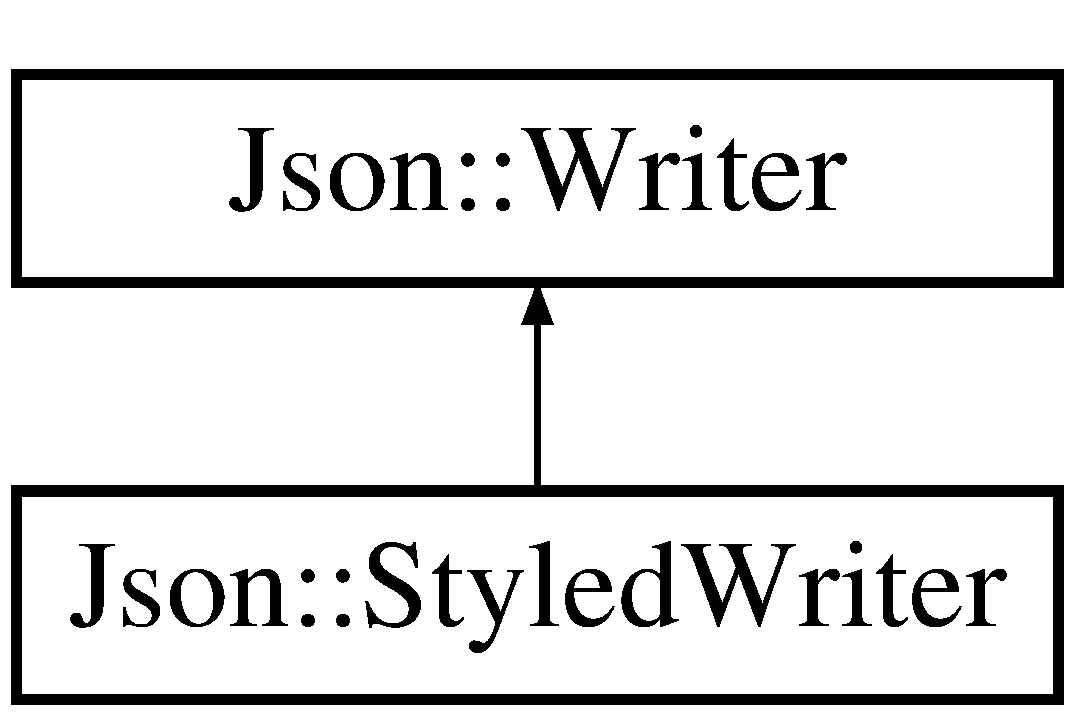
\includegraphics[height=2.000000cm]{class_json_1_1_styled_writer}
\end{center}
\end{figure}
\subsection*{Public Member Functions}
\begin{DoxyCompactItemize}
\item 
virtual std\-::string \hyperlink{class_json_1_1_styled_writer_a56f0fd80f60272b3f3c85690aae66e7d}{write} (const \hyperlink{class_json_1_1_value}{Value} \&root)
\begin{DoxyCompactList}\small\item\em Serialize a \hyperlink{class_json_1_1_value}{Value} in \href{http://www.json.org}{\tt J\-S\-O\-N} format. \end{DoxyCompactList}\end{DoxyCompactItemize}
\subsection*{Private Types}
\begin{DoxyCompactItemize}
\item 
\hypertarget{class_json_1_1_styled_writer_a0b102abcd4b7e11eb22df63921e097df}{typedef std\-::vector$<$ std\-::string $>$ {\bfseries Child\-Values}}\label{class_json_1_1_styled_writer_a0b102abcd4b7e11eb22df63921e097df}

\end{DoxyCompactItemize}
\subsection*{Private Member Functions}
\begin{DoxyCompactItemize}
\item 
\hypertarget{class_json_1_1_styled_writer_ac40143cf43f7c4a94d3d0b41e5245069}{void {\bfseries write\-Value} (const \hyperlink{class_json_1_1_value}{Value} \&value)}\label{class_json_1_1_styled_writer_ac40143cf43f7c4a94d3d0b41e5245069}

\item 
\hypertarget{class_json_1_1_styled_writer_a0618c23d62965515def15ece1e677f5d}{void {\bfseries write\-Array\-Value} (const \hyperlink{class_json_1_1_value}{Value} \&value)}\label{class_json_1_1_styled_writer_a0618c23d62965515def15ece1e677f5d}

\item 
\hypertarget{class_json_1_1_styled_writer_aa5dc671edf10b9976f1511da2271ab9d}{bool {\bfseries is\-Multine\-Array} (const \hyperlink{class_json_1_1_value}{Value} \&value)}\label{class_json_1_1_styled_writer_aa5dc671edf10b9976f1511da2271ab9d}

\item 
\hypertarget{class_json_1_1_styled_writer_aba120a1ff1b84411b32039188e8fb49f}{void {\bfseries push\-Value} (const std\-::string \&value)}\label{class_json_1_1_styled_writer_aba120a1ff1b84411b32039188e8fb49f}

\item 
\hypertarget{class_json_1_1_styled_writer_a885f4bfb5701896d60eee6716d2db7e4}{void {\bfseries write\-Indent} ()}\label{class_json_1_1_styled_writer_a885f4bfb5701896d60eee6716d2db7e4}

\item 
\hypertarget{class_json_1_1_styled_writer_a7b3cc9da3cb455ee9b2752307ac21b58}{void {\bfseries write\-With\-Indent} (const std\-::string \&value)}\label{class_json_1_1_styled_writer_a7b3cc9da3cb455ee9b2752307ac21b58}

\item 
\hypertarget{class_json_1_1_styled_writer_a0b65be6186a7c6638270990265e42b97}{void {\bfseries indent} ()}\label{class_json_1_1_styled_writer_a0b65be6186a7c6638270990265e42b97}

\item 
\hypertarget{class_json_1_1_styled_writer_acee1c9285519b573cfcb00b7e7f5a809}{void {\bfseries unindent} ()}\label{class_json_1_1_styled_writer_acee1c9285519b573cfcb00b7e7f5a809}

\item 
\hypertarget{class_json_1_1_styled_writer_ad3452c48fabf968bf3693549331ec06e}{void {\bfseries write\-Comment\-Before\-Value} (const \hyperlink{class_json_1_1_value}{Value} \&root)}\label{class_json_1_1_styled_writer_ad3452c48fabf968bf3693549331ec06e}

\item 
\hypertarget{class_json_1_1_styled_writer_ab12b274c62822fc51ec4617c6be95139}{void {\bfseries write\-Comment\-After\-Value\-On\-Same\-Line} (const \hyperlink{class_json_1_1_value}{Value} \&root)}\label{class_json_1_1_styled_writer_ab12b274c62822fc51ec4617c6be95139}

\item 
\hypertarget{class_json_1_1_styled_writer_a37a806d010f708cb68556f2666f79bdf}{bool {\bfseries has\-Comment\-For\-Value} (const \hyperlink{class_json_1_1_value}{Value} \&value)}\label{class_json_1_1_styled_writer_a37a806d010f708cb68556f2666f79bdf}

\end{DoxyCompactItemize}
\subsection*{Static Private Member Functions}
\begin{DoxyCompactItemize}
\item 
\hypertarget{class_json_1_1_styled_writer_ae5ceeb6085815461518f17a4485af571}{static std\-::string {\bfseries normalize\-E\-O\-L} (const std\-::string \&text)}\label{class_json_1_1_styled_writer_ae5ceeb6085815461518f17a4485af571}

\end{DoxyCompactItemize}
\subsection*{Private Attributes}
\begin{DoxyCompactItemize}
\item 
\hypertarget{class_json_1_1_styled_writer_a1f905495f0705365af117ec541e29fdf}{Child\-Values {\bfseries child\-Values\-\_\-}}\label{class_json_1_1_styled_writer_a1f905495f0705365af117ec541e29fdf}

\item 
\hypertarget{class_json_1_1_styled_writer_ac092c93313e7ab202b13e075d682faea}{std\-::string {\bfseries document\-\_\-}}\label{class_json_1_1_styled_writer_ac092c93313e7ab202b13e075d682faea}

\item 
\hypertarget{class_json_1_1_styled_writer_a98a33f1d4c853a4dbf87ca17499c5830}{std\-::string {\bfseries indent\-String\-\_\-}}\label{class_json_1_1_styled_writer_a98a33f1d4c853a4dbf87ca17499c5830}

\item 
\hypertarget{class_json_1_1_styled_writer_a9c8fc62cb4f3b4a6dbed470fea2aa567}{int {\bfseries right\-Margin\-\_\-}}\label{class_json_1_1_styled_writer_a9c8fc62cb4f3b4a6dbed470fea2aa567}

\item 
\hypertarget{class_json_1_1_styled_writer_ae911f06042935286c24a9fb23dba78bd}{int {\bfseries indent\-Size\-\_\-}}\label{class_json_1_1_styled_writer_ae911f06042935286c24a9fb23dba78bd}

\item 
\hypertarget{class_json_1_1_styled_writer_acaabfa48b50a8bb7fa9ce98e2ae971d9}{bool {\bfseries add\-Child\-Values\-\_\-}}\label{class_json_1_1_styled_writer_acaabfa48b50a8bb7fa9ce98e2ae971d9}

\end{DoxyCompactItemize}


\subsection{Detailed Description}
Writes a \hyperlink{class_json_1_1_value}{Value} in \href{http://www.json.org}{\tt J\-S\-O\-N} format in a human friendly way. 

The rules for line break and indent are as follow\-:
\begin{DoxyItemize}
\item Object value\-:
\begin{DoxyItemize}
\item if empty then print \{\} without indent and line break
\item if not empty the print '\{', line break \& indent, print one value per line and then unindent and line break and print '\}'.
\end{DoxyItemize}
\item Array value\-:
\begin{DoxyItemize}
\item if empty then print \mbox{[}\mbox{]} without indent and line break
\item if the array contains no object value, empty array or some other value types, and all the values fit on one lines, then print the array on a single line.
\item otherwise, it the values do not fit on one line, or the array contains object or non empty array, then print one value per line.
\end{DoxyItemize}
\end{DoxyItemize}

If the \hyperlink{class_json_1_1_value}{Value} have comments then they are outputed according to their \hyperlink{namespace_json_a4fc417c23905b2ae9e2c47d197a45351}{Comment\-Placement}.

\begin{DoxySeeAlso}{See Also}
\hyperlink{class_json_1_1_reader}{Reader}, \hyperlink{class_json_1_1_value}{Value}, \hyperlink{class_json_1_1_value_a29f3a30f7e5d3af6f38d57999bf5b480}{Value\-::set\-Comment()} 
\end{DoxySeeAlso}


\subsection{Member Function Documentation}
\hypertarget{class_json_1_1_styled_writer_a56f0fd80f60272b3f3c85690aae66e7d}{\index{Json\-::\-Styled\-Writer@{Json\-::\-Styled\-Writer}!write@{write}}
\index{write@{write}!Json::StyledWriter@{Json\-::\-Styled\-Writer}}
\subsubsection[{write}]{\setlength{\rightskip}{0pt plus 5cm}std\-::string Json\-::\-Styled\-Writer\-::write (
\begin{DoxyParamCaption}
\item[{const {\bf Value} \&}]{root}
\end{DoxyParamCaption}
)\hspace{0.3cm}{\ttfamily [virtual]}}}\label{class_json_1_1_styled_writer_a56f0fd80f60272b3f3c85690aae66e7d}


Serialize a \hyperlink{class_json_1_1_value}{Value} in \href{http://www.json.org}{\tt J\-S\-O\-N} format. 


\begin{DoxyParams}{Parameters}
{\em root} & \hyperlink{class_json_1_1_value}{Value} to serialize. \\
\hline
\end{DoxyParams}
\begin{DoxyReturn}{Returns}
String containing the J\-S\-O\-N document that represents the root value. 
\end{DoxyReturn}


Implements \hyperlink{class_json_1_1_writer}{Json\-::\-Writer}.



The documentation for this class was generated from the following files\-:\begin{DoxyCompactItemize}
\item 
/\-Users/\-Alex/github/\-A\-W\-E\-Media\-Center/\-Code/libs/json/json.\-h\item 
/\-Users/\-Alex/github/\-A\-W\-E\-Media\-Center/\-Code/libs/json/jsoncpp.\-cpp\end{DoxyCompactItemize}

\hypertarget{class_json_1_1_value}{\section{Json\-:\-:Value Class Reference}
\label{class_json_1_1_value}\index{Json\-::\-Value@{Json\-::\-Value}}
}


Represents a \href{http://www.json.org}{\tt J\-S\-O\-N} value.  




{\ttfamily \#include $<$json.\-h$>$}

\subsection*{Classes}
\begin{DoxyCompactItemize}
\item 
struct \hyperlink{struct_json_1_1_value_1_1_comment_info}{Comment\-Info}
\item 
class \hyperlink{class_json_1_1_value_1_1_c_z_string}{C\-Z\-String}
\item 
union \hyperlink{union_json_1_1_value_1_1_value_holder}{Value\-Holder}
\end{DoxyCompactItemize}
\subsection*{Public Types}
\begin{DoxyCompactItemize}
\item 
\hypertarget{class_json_1_1_value_ac61bab5a465848b57610379cc07995c3}{typedef std\-::vector$<$ std\-::string $>$ {\bfseries Members}}\label{class_json_1_1_value_ac61bab5a465848b57610379cc07995c3}

\item 
\hypertarget{class_json_1_1_value_a341cdf2e01f8b3c5b7317aa2f0768c53}{typedef \hyperlink{class_json_1_1_value_iterator}{Value\-Iterator} {\bfseries iterator}}\label{class_json_1_1_value_a341cdf2e01f8b3c5b7317aa2f0768c53}

\item 
\hypertarget{class_json_1_1_value_af92282ca92b58b320debd486afb7696a}{typedef \hyperlink{class_json_1_1_value_const_iterator}{Value\-Const\-Iterator} {\bfseries const\-\_\-iterator}}\label{class_json_1_1_value_af92282ca92b58b320debd486afb7696a}

\item 
\hypertarget{class_json_1_1_value_a0933d59b45793ae4aade1757c322a98d}{typedef Json\-::\-U\-Int {\bfseries U\-Int}}\label{class_json_1_1_value_a0933d59b45793ae4aade1757c322a98d}

\item 
\hypertarget{class_json_1_1_value_abdf7a7ff73eb130ffcab28504ffdb405}{typedef Json\-::\-Int {\bfseries Int}}\label{class_json_1_1_value_abdf7a7ff73eb130ffcab28504ffdb405}

\item 
\hypertarget{class_json_1_1_value_a8b62564be8c087c6d18de180ff4e13e3}{typedef Json\-::\-U\-Int64 {\bfseries U\-Int64}}\label{class_json_1_1_value_a8b62564be8c087c6d18de180ff4e13e3}

\item 
\hypertarget{class_json_1_1_value_a1b86af9f85f0f1baa972c3319fa22695}{typedef Json\-::\-Int64 {\bfseries Int64}}\label{class_json_1_1_value_a1b86af9f85f0f1baa972c3319fa22695}

\item 
\hypertarget{class_json_1_1_value_a1cbb82642ed05109b9833e49f042ece7}{typedef Json\-::\-Largest\-Int {\bfseries Largest\-Int}}\label{class_json_1_1_value_a1cbb82642ed05109b9833e49f042ece7}

\item 
\hypertarget{class_json_1_1_value_a6682a3684d635e03fc06ba229fa24eec}{typedef Json\-::\-Largest\-U\-Int {\bfseries Largest\-U\-Int}}\label{class_json_1_1_value_a6682a3684d635e03fc06ba229fa24eec}

\item 
\hypertarget{class_json_1_1_value_a184a91566cccca7b819240f0d5561c7d}{typedef Json\-::\-Array\-Index {\bfseries Array\-Index}}\label{class_json_1_1_value_a184a91566cccca7b819240f0d5561c7d}

\item 
\hypertarget{class_json_1_1_value_a08b6c80c3af7071d908dabf044de5388}{typedef std\-::map$<$ \hyperlink{class_json_1_1_value_1_1_c_z_string}{C\-Z\-String}, \hyperlink{class_json_1_1_value}{Value} $>$ {\bfseries Object\-Values}}\label{class_json_1_1_value_a08b6c80c3af7071d908dabf044de5388}

\end{DoxyCompactItemize}
\subsection*{Public Member Functions}
\begin{DoxyCompactItemize}
\item 
\hyperlink{class_json_1_1_value_ada6ba1369448fb0240bccc36efaa46f7}{Value} (\hyperlink{namespace_json_a7d654b75c16a57007925868e38212b4e}{Value\-Type} type=\hyperlink{namespace_json_a7d654b75c16a57007925868e38212b4ea7d9899633b4409bd3fc107e6737f8391}{null\-Value})
\begin{DoxyCompactList}\small\item\em Create a default \hyperlink{class_json_1_1_value}{Value} of the given type. \end{DoxyCompactList}\item 
\hypertarget{class_json_1_1_value_a4744ae571fcf34f4b16a2257b3b3b585}{{\bfseries Value} (Int value)}\label{class_json_1_1_value_a4744ae571fcf34f4b16a2257b3b3b585}

\item 
\hypertarget{class_json_1_1_value_ae67a857b01286e3499a87e95be848d20}{{\bfseries Value} (U\-Int value)}\label{class_json_1_1_value_ae67a857b01286e3499a87e95be848d20}

\item 
\hypertarget{class_json_1_1_value_ab1cdc3d9a4d4cc03fa01439d43ceb1b5}{{\bfseries Value} (Int64 value)}\label{class_json_1_1_value_ab1cdc3d9a4d4cc03fa01439d43ceb1b5}

\item 
\hypertarget{class_json_1_1_value_a8adda58d5ae17bf7ca6a53bab4a7b69c}{{\bfseries Value} (U\-Int64 value)}\label{class_json_1_1_value_a8adda58d5ae17bf7ca6a53bab4a7b69c}

\item 
\hypertarget{class_json_1_1_value_a32228cc84d83200cca8441451997996c}{{\bfseries Value} (double value)}\label{class_json_1_1_value_a32228cc84d83200cca8441451997996c}

\item 
\hypertarget{class_json_1_1_value_ad87b849356816aca75995dd07302e49d}{{\bfseries Value} (const char $\ast$value)}\label{class_json_1_1_value_ad87b849356816aca75995dd07302e49d}

\item 
\hypertarget{class_json_1_1_value_a13e567d467bb1e699d71e27a76b0e988}{{\bfseries Value} (const char $\ast$begin\-Value, const char $\ast$end\-Value)}\label{class_json_1_1_value_a13e567d467bb1e699d71e27a76b0e988}

\item 
\hyperlink{class_json_1_1_value_a081830e95f88a37054da7e46c65b0766}{Value} (const \hyperlink{class_json_1_1_static_string}{Static\-String} \&value)
\begin{DoxyCompactList}\small\item\em Constructs a value from a static string. \end{DoxyCompactList}\item 
\hypertarget{class_json_1_1_value_aa4501dd4edf3ce3d5145fc656f088b21}{{\bfseries Value} (const std\-::string \&value)}\label{class_json_1_1_value_aa4501dd4edf3ce3d5145fc656f088b21}

\item 
\hypertarget{class_json_1_1_value_a350a31ea4a30d384994b0bc010b17495}{{\bfseries Value} (bool value)}\label{class_json_1_1_value_a350a31ea4a30d384994b0bc010b17495}

\item 
\hypertarget{class_json_1_1_value_a436dfd3670f95fd665f680eba5cebcf0}{{\bfseries Value} (const \hyperlink{class_json_1_1_value}{Value} \&other)}\label{class_json_1_1_value_a436dfd3670f95fd665f680eba5cebcf0}

\item 
\hypertarget{class_json_1_1_value_ade21ab9710b64fee954b5fcceb0d37dd}{\hyperlink{class_json_1_1_value}{Value} \& {\bfseries operator=} (const \hyperlink{class_json_1_1_value}{Value} \&other)}\label{class_json_1_1_value_ade21ab9710b64fee954b5fcceb0d37dd}

\item 
void \hyperlink{class_json_1_1_value_aab841120d78e296e1bc06a373345e822}{swap} (\hyperlink{class_json_1_1_value}{Value} \&other)
\item 
\hypertarget{class_json_1_1_value_a695ef31fad36b4712918b3ff80158479}{\hyperlink{namespace_json_a7d654b75c16a57007925868e38212b4e}{Value\-Type} {\bfseries type} () const }\label{class_json_1_1_value_a695ef31fad36b4712918b3ff80158479}

\item 
\hypertarget{class_json_1_1_value_af0ad8aa027575c3277296458f3fb7b0a}{bool {\bfseries operator$<$} (const \hyperlink{class_json_1_1_value}{Value} \&other) const }\label{class_json_1_1_value_af0ad8aa027575c3277296458f3fb7b0a}

\item 
\hypertarget{class_json_1_1_value_afb99dd3628fe44244b32007f9b4f369a}{bool {\bfseries operator$<$=} (const \hyperlink{class_json_1_1_value}{Value} \&other) const }\label{class_json_1_1_value_afb99dd3628fe44244b32007f9b4f369a}

\item 
\hypertarget{class_json_1_1_value_acc13fc47d55abd6e2327b090b83d2911}{bool {\bfseries operator$>$=} (const \hyperlink{class_json_1_1_value}{Value} \&other) const }\label{class_json_1_1_value_acc13fc47d55abd6e2327b090b83d2911}

\item 
\hypertarget{class_json_1_1_value_a3124a26067bdfde9571bc89527fc6931}{bool {\bfseries operator$>$} (const \hyperlink{class_json_1_1_value}{Value} \&other) const }\label{class_json_1_1_value_a3124a26067bdfde9571bc89527fc6931}

\item 
\hypertarget{class_json_1_1_value_a14363dda23a6ae2def9afd1590ae85d3}{bool {\bfseries operator==} (const \hyperlink{class_json_1_1_value}{Value} \&other) const }\label{class_json_1_1_value_a14363dda23a6ae2def9afd1590ae85d3}

\item 
\hypertarget{class_json_1_1_value_ad0f12d2a4ab74bbef08a05504b2cb81d}{bool {\bfseries operator!=} (const \hyperlink{class_json_1_1_value}{Value} \&other) const }\label{class_json_1_1_value_ad0f12d2a4ab74bbef08a05504b2cb81d}

\item 
\hypertarget{class_json_1_1_value_a899214ed2253d3f4f061b922b0e622b5}{int {\bfseries compare} (const \hyperlink{class_json_1_1_value}{Value} \&other) const }\label{class_json_1_1_value_a899214ed2253d3f4f061b922b0e622b5}

\item 
\hypertarget{class_json_1_1_value_a5b7da48b163bcec63b1424f1608b7da6}{const char $\ast$ {\bfseries as\-C\-String} () const }\label{class_json_1_1_value_a5b7da48b163bcec63b1424f1608b7da6}

\item 
\hypertarget{class_json_1_1_value_a03ee3d5df576640c93ba683f140828bd}{std\-::string {\bfseries as\-String} () const }\label{class_json_1_1_value_a03ee3d5df576640c93ba683f140828bd}

\item 
\hypertarget{class_json_1_1_value_ac786e35b860b1d700cb3d3e56dd6a235}{Int {\bfseries as\-Int} () const }\label{class_json_1_1_value_ac786e35b860b1d700cb3d3e56dd6a235}

\item 
\hypertarget{class_json_1_1_value_a2019d1bd296b89356c1b0da5970c918c}{U\-Int {\bfseries as\-U\-Int} () const }\label{class_json_1_1_value_a2019d1bd296b89356c1b0da5970c918c}

\item 
\hypertarget{class_json_1_1_value_a7f739b55aef060f4ab6360bfe1912b77}{Int64 {\bfseries as\-Int64} () const }\label{class_json_1_1_value_a7f739b55aef060f4ab6360bfe1912b77}

\item 
\hypertarget{class_json_1_1_value_a65acdab039f60ff0da15e622f2e17739}{U\-Int64 {\bfseries as\-U\-Int64} () const }\label{class_json_1_1_value_a65acdab039f60ff0da15e622f2e17739}

\item 
\hypertarget{class_json_1_1_value_a3786bb100c5cf9a98eb6d13784968956}{Largest\-Int {\bfseries as\-Largest\-Int} () const }\label{class_json_1_1_value_a3786bb100c5cf9a98eb6d13784968956}

\item 
\hypertarget{class_json_1_1_value_a692b88345a745b2f89ca5d94b52e94d4}{Largest\-U\-Int {\bfseries as\-Largest\-U\-Int} () const }\label{class_json_1_1_value_a692b88345a745b2f89ca5d94b52e94d4}

\item 
\hypertarget{class_json_1_1_value_ac2128d7080499daf8c5b1c71da243f63}{float {\bfseries as\-Float} () const }\label{class_json_1_1_value_ac2128d7080499daf8c5b1c71da243f63}

\item 
\hypertarget{class_json_1_1_value_a33434ed1c0217a34d04c95fa5342fd37}{double {\bfseries as\-Double} () const }\label{class_json_1_1_value_a33434ed1c0217a34d04c95fa5342fd37}

\item 
\hypertarget{class_json_1_1_value_a7402c797285c020566c3db5f8ae4e940}{bool {\bfseries as\-Bool} () const }\label{class_json_1_1_value_a7402c797285c020566c3db5f8ae4e940}

\item 
\hypertarget{class_json_1_1_value_aeb9ad8b1bb91bdd72203dc884b3f4362}{bool {\bfseries is\-Null} () const }\label{class_json_1_1_value_aeb9ad8b1bb91bdd72203dc884b3f4362}

\item 
\hypertarget{class_json_1_1_value_a3c3716cc7a0216cb1b654bb8f61c8d13}{bool {\bfseries is\-Bool} () const }\label{class_json_1_1_value_a3c3716cc7a0216cb1b654bb8f61c8d13}

\item 
\hypertarget{class_json_1_1_value_ab0df4746d6787d2ce1db1a156c118f14}{bool {\bfseries is\-Int} () const }\label{class_json_1_1_value_ab0df4746d6787d2ce1db1a156c118f14}

\item 
\hypertarget{class_json_1_1_value_ae814ca1796fe2d43ac09898b70213989}{bool {\bfseries is\-U\-Int} () const }\label{class_json_1_1_value_ae814ca1796fe2d43ac09898b70213989}

\item 
\hypertarget{class_json_1_1_value_aec4f74ef7b776b1d9c8a10fc3bb4add5}{bool {\bfseries is\-Integral} () const }\label{class_json_1_1_value_aec4f74ef7b776b1d9c8a10fc3bb4add5}

\item 
\hypertarget{class_json_1_1_value_a0ea567fa51fc808851698bef59b43626}{bool {\bfseries is\-Double} () const }\label{class_json_1_1_value_a0ea567fa51fc808851698bef59b43626}

\item 
\hypertarget{class_json_1_1_value_a8ce848900e2e8fa23a41fcc2c1409fab}{bool {\bfseries is\-Numeric} () const }\label{class_json_1_1_value_a8ce848900e2e8fa23a41fcc2c1409fab}

\item 
\hypertarget{class_json_1_1_value_a06c01d7c1e8151a5844b595ab00f46c7}{bool {\bfseries is\-String} () const }\label{class_json_1_1_value_a06c01d7c1e8151a5844b595ab00f46c7}

\item 
\hypertarget{class_json_1_1_value_ac8c898f93543e55b67418f94bced20af}{bool {\bfseries is\-Array} () const }\label{class_json_1_1_value_ac8c898f93543e55b67418f94bced20af}

\item 
\hypertarget{class_json_1_1_value_a80cffaa0402b80317c0437216bbb6d92}{bool {\bfseries is\-Object} () const }\label{class_json_1_1_value_a80cffaa0402b80317c0437216bbb6d92}

\item 
\hypertarget{class_json_1_1_value_a7ec153803631a27abf58cba2bb1af70c}{bool {\bfseries is\-Convertible\-To} (\hyperlink{namespace_json_a7d654b75c16a57007925868e38212b4e}{Value\-Type} other) const }\label{class_json_1_1_value_a7ec153803631a27abf58cba2bb1af70c}

\item 
\hypertarget{class_json_1_1_value_a4ca8ee6c48a34ca6c2f131956bab5e05}{Array\-Index \hyperlink{class_json_1_1_value_a4ca8ee6c48a34ca6c2f131956bab5e05}{size} () const }\label{class_json_1_1_value_a4ca8ee6c48a34ca6c2f131956bab5e05}

\begin{DoxyCompactList}\small\item\em Number of values in array or object. \end{DoxyCompactList}\item 
\hypertarget{class_json_1_1_value_a99c42d3ff8495dad1e91b43e66553c36}{bool \hyperlink{class_json_1_1_value_a99c42d3ff8495dad1e91b43e66553c36}{empty} () const }\label{class_json_1_1_value_a99c42d3ff8495dad1e91b43e66553c36}

\begin{DoxyCompactList}\small\item\em Return true if empty array, empty object, or null; otherwise, false. \end{DoxyCompactList}\item 
\hypertarget{class_json_1_1_value_a021ab0d15a807fbe051446c9c545ab61}{bool \hyperlink{class_json_1_1_value_a021ab0d15a807fbe051446c9c545ab61}{operator!} () const }\label{class_json_1_1_value_a021ab0d15a807fbe051446c9c545ab61}

\begin{DoxyCompactList}\small\item\em Return is\-Null() \end{DoxyCompactList}\item 
void \hyperlink{class_json_1_1_value_a501a4d67e6c875255c2ecc03ccd2019b}{clear} ()
\item 
void \hyperlink{class_json_1_1_value_aa284353271ada427dbfa04a42f2be407}{resize} (Array\-Index \hyperlink{class_json_1_1_value_a4ca8ee6c48a34ca6c2f131956bab5e05}{size})
\item 
\hyperlink{class_json_1_1_value}{Value} \& \hyperlink{class_json_1_1_value_a7d99f5dba388cdaa152ce6ef933d64ef}{operator\mbox{[}$\,$\mbox{]}} (Array\-Index index)
\item 
\hyperlink{class_json_1_1_value}{Value} \& \hyperlink{class_json_1_1_value_ac9182982c361e0ab621134d406e5f250}{operator\mbox{[}$\,$\mbox{]}} (int index)
\item 
const \hyperlink{class_json_1_1_value}{Value} \& \hyperlink{class_json_1_1_value_af151919e8947c430e34bed2b0b128601}{operator\mbox{[}$\,$\mbox{]}} (Array\-Index index) const 
\item 
const \hyperlink{class_json_1_1_value}{Value} \& \hyperlink{class_json_1_1_value_af9e02b38f4e63e491c300c20b275bdd7}{operator\mbox{[}$\,$\mbox{]}} (int index) const 
\item 
\hyperlink{class_json_1_1_value}{Value} \hyperlink{class_json_1_1_value_a28282c9b76fa031eba7a1843c47c16fe}{get} (Array\-Index index, const \hyperlink{class_json_1_1_value}{Value} \&default\-Value) const 
\item 
\hypertarget{class_json_1_1_value_aaa82ebb4b730ea1567d310874f47d147}{bool \hyperlink{class_json_1_1_value_aaa82ebb4b730ea1567d310874f47d147}{is\-Valid\-Index} (Array\-Index index) const }\label{class_json_1_1_value_aaa82ebb4b730ea1567d310874f47d147}

\begin{DoxyCompactList}\small\item\em Return true if index $<$ \hyperlink{class_json_1_1_value_a4ca8ee6c48a34ca6c2f131956bab5e05}{size()}. \end{DoxyCompactList}\item 
\hyperlink{class_json_1_1_value}{Value} \& \hyperlink{class_json_1_1_value_a7e49ac977e4bcf59745a09d426669f75}{append} (const \hyperlink{class_json_1_1_value}{Value} \&value)
\begin{DoxyCompactList}\small\item\em Append value to array at the end. \end{DoxyCompactList}\item 
\hypertarget{class_json_1_1_value_acb912f4ec40a25ea6eb387730885f3d9}{\hyperlink{class_json_1_1_value}{Value} \& \hyperlink{class_json_1_1_value_acb912f4ec40a25ea6eb387730885f3d9}{operator\mbox{[}$\,$\mbox{]}} (const char $\ast$key)}\label{class_json_1_1_value_acb912f4ec40a25ea6eb387730885f3d9}

\begin{DoxyCompactList}\small\item\em Access an object value by name, create a null member if it does not exist. \end{DoxyCompactList}\item 
\hypertarget{class_json_1_1_value_ae5f73ffc7a039bca81b7ca771bc5db55}{const \hyperlink{class_json_1_1_value}{Value} \& \hyperlink{class_json_1_1_value_ae5f73ffc7a039bca81b7ca771bc5db55}{operator\mbox{[}$\,$\mbox{]}} (const char $\ast$key) const }\label{class_json_1_1_value_ae5f73ffc7a039bca81b7ca771bc5db55}

\begin{DoxyCompactList}\small\item\em Access an object value by name, returns null if there is no member with that name. \end{DoxyCompactList}\item 
\hypertarget{class_json_1_1_value_ae511c7d46bf457412fb55c9471af9f50}{\hyperlink{class_json_1_1_value}{Value} \& \hyperlink{class_json_1_1_value_ae511c7d46bf457412fb55c9471af9f50}{operator\mbox{[}$\,$\mbox{]}} (const std\-::string \&key)}\label{class_json_1_1_value_ae511c7d46bf457412fb55c9471af9f50}

\begin{DoxyCompactList}\small\item\em Access an object value by name, create a null member if it does not exist. \end{DoxyCompactList}\item 
\hypertarget{class_json_1_1_value_ac14123afaf12d953aad75ec2610fbb85}{const \hyperlink{class_json_1_1_value}{Value} \& \hyperlink{class_json_1_1_value_ac14123afaf12d953aad75ec2610fbb85}{operator\mbox{[}$\,$\mbox{]}} (const std\-::string \&key) const }\label{class_json_1_1_value_ac14123afaf12d953aad75ec2610fbb85}

\begin{DoxyCompactList}\small\item\em Access an object value by name, returns null if there is no member with that name. \end{DoxyCompactList}\item 
\hyperlink{class_json_1_1_value}{Value} \& \hyperlink{class_json_1_1_value_ac3763d7d315ca65dc188e273722f7955}{operator\mbox{[}$\,$\mbox{]}} (const \hyperlink{class_json_1_1_static_string}{Static\-String} \&key)
\begin{DoxyCompactList}\small\item\em Access an object value by name, create a null member if it does not exist. \end{DoxyCompactList}\item 
\hypertarget{class_json_1_1_value_ab76b3323cde14c7db20676d07b260ce7}{\hyperlink{class_json_1_1_value}{Value} \hyperlink{class_json_1_1_value_ab76b3323cde14c7db20676d07b260ce7}{get} (const char $\ast$key, const \hyperlink{class_json_1_1_value}{Value} \&default\-Value) const }\label{class_json_1_1_value_ab76b3323cde14c7db20676d07b260ce7}

\begin{DoxyCompactList}\small\item\em Return the member named key if it exist, default\-Value otherwise. \end{DoxyCompactList}\item 
\hypertarget{class_json_1_1_value_a54a34264356e01ee9c21a75ccfc809e9}{\hyperlink{class_json_1_1_value}{Value} \hyperlink{class_json_1_1_value_a54a34264356e01ee9c21a75ccfc809e9}{get} (const std\-::string \&key, const \hyperlink{class_json_1_1_value}{Value} \&default\-Value) const }\label{class_json_1_1_value_a54a34264356e01ee9c21a75ccfc809e9}

\begin{DoxyCompactList}\small\item\em Return the member named key if it exist, default\-Value otherwise. \end{DoxyCompactList}\item 
\hyperlink{class_json_1_1_value}{Value} \hyperlink{class_json_1_1_value_aa52f7873b95d29627d6e83ba96f69aaa}{remove\-Member} (const char $\ast$key)
\begin{DoxyCompactList}\small\item\em Remove and return the named member. \end{DoxyCompactList}\item 
\hypertarget{class_json_1_1_value_ae1f95f7ca3906e6bcc2a7be93210ecba}{\hyperlink{class_json_1_1_value}{Value} \hyperlink{class_json_1_1_value_ae1f95f7ca3906e6bcc2a7be93210ecba}{remove\-Member} (const std\-::string \&key)}\label{class_json_1_1_value_ae1f95f7ca3906e6bcc2a7be93210ecba}

\begin{DoxyCompactList}\small\item\em Same as \hyperlink{class_json_1_1_value_aa52f7873b95d29627d6e83ba96f69aaa}{remove\-Member(const char$\ast$)} \end{DoxyCompactList}\item 
\hypertarget{class_json_1_1_value_a196defba501d70ea2b6793afb04108e3}{bool \hyperlink{class_json_1_1_value_a196defba501d70ea2b6793afb04108e3}{is\-Member} (const char $\ast$key) const }\label{class_json_1_1_value_a196defba501d70ea2b6793afb04108e3}

\begin{DoxyCompactList}\small\item\em Return true if the object has a member named key. \end{DoxyCompactList}\item 
\hypertarget{class_json_1_1_value_af728b5738aaa133f3aad2e39dc4f415e}{bool \hyperlink{class_json_1_1_value_af728b5738aaa133f3aad2e39dc4f415e}{is\-Member} (const std\-::string \&key) const }\label{class_json_1_1_value_af728b5738aaa133f3aad2e39dc4f415e}

\begin{DoxyCompactList}\small\item\em Return true if the object has a member named key. \end{DoxyCompactList}\item 
Members \hyperlink{class_json_1_1_value_a30fa08af88f2d0a038b22ba9f4e88b2a}{get\-Member\-Names} () const 
\begin{DoxyCompactList}\small\item\em Return a list of the member names. \end{DoxyCompactList}\item 
\hypertarget{class_json_1_1_value_a29f3a30f7e5d3af6f38d57999bf5b480}{void \hyperlink{class_json_1_1_value_a29f3a30f7e5d3af6f38d57999bf5b480}{set\-Comment} (const char $\ast$comment, \hyperlink{namespace_json_a4fc417c23905b2ae9e2c47d197a45351}{Comment\-Placement} placement)}\label{class_json_1_1_value_a29f3a30f7e5d3af6f38d57999bf5b480}

\begin{DoxyCompactList}\small\item\em Comments must be //... or /$\ast$ ... $\ast$/. \end{DoxyCompactList}\item 
\hypertarget{class_json_1_1_value_a6d68a2e7d4e1e317cd9e812e12181689}{void \hyperlink{class_json_1_1_value_a6d68a2e7d4e1e317cd9e812e12181689}{set\-Comment} (const std\-::string \&comment, \hyperlink{namespace_json_a4fc417c23905b2ae9e2c47d197a45351}{Comment\-Placement} placement)}\label{class_json_1_1_value_a6d68a2e7d4e1e317cd9e812e12181689}

\begin{DoxyCompactList}\small\item\em Comments must be //... or /$\ast$ ... $\ast$/. \end{DoxyCompactList}\item 
\hypertarget{class_json_1_1_value_a06567a00363cab9601be7e31336db03a}{bool {\bfseries has\-Comment} (\hyperlink{namespace_json_a4fc417c23905b2ae9e2c47d197a45351}{Comment\-Placement} placement) const }\label{class_json_1_1_value_a06567a00363cab9601be7e31336db03a}

\item 
\hypertarget{class_json_1_1_value_aa1e105b5d7f55d6e42f4fb2f3674116f}{std\-::string \hyperlink{class_json_1_1_value_aa1e105b5d7f55d6e42f4fb2f3674116f}{get\-Comment} (\hyperlink{namespace_json_a4fc417c23905b2ae9e2c47d197a45351}{Comment\-Placement} placement) const }\label{class_json_1_1_value_aa1e105b5d7f55d6e42f4fb2f3674116f}

\begin{DoxyCompactList}\small\item\em Include delimiters and embedded newlines. \end{DoxyCompactList}\item 
\hypertarget{class_json_1_1_value_a05357cf78959b790337fae4e5580ee4f}{std\-::string {\bfseries to\-Styled\-String} () const }\label{class_json_1_1_value_a05357cf78959b790337fae4e5580ee4f}

\item 
\hypertarget{class_json_1_1_value_ac12df0d6980600c5bac908ed0f64856e}{\hyperlink{class_json_1_1_value_const_iterator}{const\-\_\-iterator} {\bfseries begin} () const }\label{class_json_1_1_value_ac12df0d6980600c5bac908ed0f64856e}

\item 
\hypertarget{class_json_1_1_value_a596da1926b2f2a4056bff2edb713eb0b}{\hyperlink{class_json_1_1_value_const_iterator}{const\-\_\-iterator} {\bfseries end} () const }\label{class_json_1_1_value_a596da1926b2f2a4056bff2edb713eb0b}

\item 
\hypertarget{class_json_1_1_value_a2d45bb2e68e8f22fe356d7d955ebd3c9}{\hyperlink{class_json_1_1_value_iterator}{iterator} {\bfseries begin} ()}\label{class_json_1_1_value_a2d45bb2e68e8f22fe356d7d955ebd3c9}

\item 
\hypertarget{class_json_1_1_value_a2f961eff73f7f79cd29260b6cbd42558}{\hyperlink{class_json_1_1_value_iterator}{iterator} {\bfseries end} ()}\label{class_json_1_1_value_a2f961eff73f7f79cd29260b6cbd42558}

\end{DoxyCompactItemize}
\subsection*{Static Public Attributes}
\begin{DoxyCompactItemize}
\item 
\hypertarget{class_json_1_1_value_a57d8e12306732c80d1719206fcc59b22}{static const \hyperlink{class_json_1_1_value}{Value} {\bfseries null}}\label{class_json_1_1_value_a57d8e12306732c80d1719206fcc59b22}

\item 
\hypertarget{class_json_1_1_value_af91df130daa50dd43d2cd89e6ee67706}{static const Largest\-Int \hyperlink{class_json_1_1_value_af91df130daa50dd43d2cd89e6ee67706}{min\-Largest\-Int} = Largest\-Int( $\sim$(Largest\-U\-Int(-\/1)/2) )}\label{class_json_1_1_value_af91df130daa50dd43d2cd89e6ee67706}

\begin{DoxyCompactList}\small\item\em Minimum signed integer value that can be stored in a \hyperlink{class_json_1_1_value}{Json\-::\-Value}. \end{DoxyCompactList}\item 
\hypertarget{class_json_1_1_value_a8b4977696f13296fa8755c7953fafb2f}{static const Largest\-Int \hyperlink{class_json_1_1_value_a8b4977696f13296fa8755c7953fafb2f}{max\-Largest\-Int} = Largest\-Int( Largest\-U\-Int(-\/1)/2 )}\label{class_json_1_1_value_a8b4977696f13296fa8755c7953fafb2f}

\begin{DoxyCompactList}\small\item\em Maximum signed integer value that can be stored in a \hyperlink{class_json_1_1_value}{Json\-::\-Value}. \end{DoxyCompactList}\item 
\hypertarget{class_json_1_1_value_a8ddb32d9d55fa5323ae5135639dc2e31}{static const Largest\-U\-Int \hyperlink{class_json_1_1_value_a8ddb32d9d55fa5323ae5135639dc2e31}{max\-Largest\-U\-Int} = Largest\-U\-Int(-\/1)}\label{class_json_1_1_value_a8ddb32d9d55fa5323ae5135639dc2e31}

\begin{DoxyCompactList}\small\item\em Maximum unsigned integer value that can be stored in a \hyperlink{class_json_1_1_value}{Json\-::\-Value}. \end{DoxyCompactList}\item 
\hypertarget{class_json_1_1_value_a7df8a39e2502b8c92a6a41e3d752d2c8}{static const Int \hyperlink{class_json_1_1_value_a7df8a39e2502b8c92a6a41e3d752d2c8}{min\-Int} = Int( $\sim$(U\-Int(-\/1)/2) )}\label{class_json_1_1_value_a7df8a39e2502b8c92a6a41e3d752d2c8}

\begin{DoxyCompactList}\small\item\em Minimum signed int value that can be stored in a \hyperlink{class_json_1_1_value}{Json\-::\-Value}. \end{DoxyCompactList}\item 
\hypertarget{class_json_1_1_value_a978c799a8af3114ef7dab6fd0a310a1b}{static const Int \hyperlink{class_json_1_1_value_a978c799a8af3114ef7dab6fd0a310a1b}{max\-Int} = Int( U\-Int(-\/1)/2 )}\label{class_json_1_1_value_a978c799a8af3114ef7dab6fd0a310a1b}

\begin{DoxyCompactList}\small\item\em Maximum signed int value that can be stored in a \hyperlink{class_json_1_1_value}{Json\-::\-Value}. \end{DoxyCompactList}\item 
\hypertarget{class_json_1_1_value_ac79e63ee68d3aa914bfd6988be669b87}{static const U\-Int \hyperlink{class_json_1_1_value_ac79e63ee68d3aa914bfd6988be669b87}{max\-U\-Int} = U\-Int(-\/1)}\label{class_json_1_1_value_ac79e63ee68d3aa914bfd6988be669b87}

\begin{DoxyCompactList}\small\item\em Maximum unsigned int value that can be stored in a \hyperlink{class_json_1_1_value}{Json\-::\-Value}. \end{DoxyCompactList}\item 
\hypertarget{class_json_1_1_value_a815ef899bc312c93bc426511acfe31a7}{static const Int64 \hyperlink{class_json_1_1_value_a815ef899bc312c93bc426511acfe31a7}{min\-Int64} = Int64( $\sim$(U\-Int64(-\/1)/2) )}\label{class_json_1_1_value_a815ef899bc312c93bc426511acfe31a7}

\begin{DoxyCompactList}\small\item\em Minimum signed 64 bits int value that can be stored in a \hyperlink{class_json_1_1_value}{Json\-::\-Value}. \end{DoxyCompactList}\item 
\hypertarget{class_json_1_1_value_a4492634870b8c5709ce967b384ac6006}{static const Int64 \hyperlink{class_json_1_1_value_a4492634870b8c5709ce967b384ac6006}{max\-Int64} = Int64( U\-Int64(-\/1)/2 )}\label{class_json_1_1_value_a4492634870b8c5709ce967b384ac6006}

\begin{DoxyCompactList}\small\item\em Maximum signed 64 bits int value that can be stored in a \hyperlink{class_json_1_1_value}{Json\-::\-Value}. \end{DoxyCompactList}\item 
\hypertarget{class_json_1_1_value_ae1eb89c305c39516696ff305cffa01da}{static const U\-Int64 \hyperlink{class_json_1_1_value_ae1eb89c305c39516696ff305cffa01da}{max\-U\-Int64} = U\-Int64(-\/1)}\label{class_json_1_1_value_ae1eb89c305c39516696ff305cffa01da}

\begin{DoxyCompactList}\small\item\em Maximum unsigned 64 bits int value that can be stored in a \hyperlink{class_json_1_1_value}{Json\-::\-Value}. \end{DoxyCompactList}\end{DoxyCompactItemize}
\subsection*{Private Member Functions}
\begin{DoxyCompactItemize}
\item 
\hypertarget{class_json_1_1_value_a12a3aded9e1478636ebf9a80843b4f5f}{\hyperlink{class_json_1_1_value}{Value} \& {\bfseries resolve\-Reference} (const char $\ast$key, bool is\-Static)}\label{class_json_1_1_value_a12a3aded9e1478636ebf9a80843b4f5f}

\end{DoxyCompactItemize}
\subsection*{Private Attributes}
\begin{DoxyCompactItemize}
\item 
\hypertarget{class_json_1_1_value_aef578244546212705b9f81eb84d7e151}{union \hyperlink{union_json_1_1_value_1_1_value_holder}{Json\-::\-Value\-::\-Value\-Holder} {\bfseries value\-\_\-}}\label{class_json_1_1_value_aef578244546212705b9f81eb84d7e151}

\item 
\hypertarget{class_json_1_1_value_abd222c2536dc88bf330dedcd076d2356}{\hyperlink{namespace_json_a7d654b75c16a57007925868e38212b4e}{Value\-Type} {\bfseries type\-\_\-}\-: 8}\label{class_json_1_1_value_abd222c2536dc88bf330dedcd076d2356}

\item 
\hypertarget{class_json_1_1_value_af728318d6cfa3e93dcc554d821447646}{int {\bfseries allocated\-\_\-}\-: 1}\label{class_json_1_1_value_af728318d6cfa3e93dcc554d821447646}

\item 
\hypertarget{class_json_1_1_value_a2016564cabc7a29208e97bd0b782a4e4}{\hyperlink{struct_json_1_1_value_1_1_comment_info}{Comment\-Info} $\ast$ {\bfseries comments\-\_\-}}\label{class_json_1_1_value_a2016564cabc7a29208e97bd0b782a4e4}

\end{DoxyCompactItemize}
\subsection*{Friends}
\begin{DoxyCompactItemize}
\item 
\hypertarget{class_json_1_1_value_ad016df56489e5d360735457afba2f649}{class {\bfseries Value\-Iterator\-Base}}\label{class_json_1_1_value_ad016df56489e5d360735457afba2f649}

\end{DoxyCompactItemize}


\subsection{Detailed Description}
Represents a \href{http://www.json.org}{\tt J\-S\-O\-N} value. 

This class is a discriminated union wrapper that can represents a\-:
\begin{DoxyItemize}
\item signed integer \mbox{[}range\-: \hyperlink{class_json_1_1_value_a7df8a39e2502b8c92a6a41e3d752d2c8}{Value\-::min\-Int} -\/ \hyperlink{class_json_1_1_value_a978c799a8af3114ef7dab6fd0a310a1b}{Value\-::max\-Int}\mbox{]}
\item unsigned integer (range\-: 0 -\/ \hyperlink{class_json_1_1_value_ac79e63ee68d3aa914bfd6988be669b87}{Value\-::max\-U\-Int})
\item double
\item U\-T\-F-\/8 string
\item boolean
\item 'null'
\item an ordered list of \hyperlink{class_json_1_1_value}{Value}
\item collection of name/value pairs (javascript object)
\end{DoxyItemize}

The type of the held value is represented by a \hyperlink{namespace_json_a7d654b75c16a57007925868e38212b4e}{Value\-Type} and can be obtained using type().

values of an \hyperlink{namespace_json_a7d654b75c16a57007925868e38212b4eae8386dcfc36d1ae897745f7b4f77a1f6}{object\-Value} or \hyperlink{namespace_json_a7d654b75c16a57007925868e38212b4eadc8f264f36b55b063c78126b335415f4}{array\-Value} can be accessed using \hyperlink{class_json_1_1_value_a7d99f5dba388cdaa152ce6ef933d64ef}{operator\mbox{[}$\,$\mbox{]}()} methods. Non const methods will automatically create the a \hyperlink{namespace_json_a7d654b75c16a57007925868e38212b4ea7d9899633b4409bd3fc107e6737f8391}{null\-Value} element if it does not exist. The sequence of an \hyperlink{namespace_json_a7d654b75c16a57007925868e38212b4eadc8f264f36b55b063c78126b335415f4}{array\-Value} will be automatically resize and initialized with \hyperlink{namespace_json_a7d654b75c16a57007925868e38212b4ea7d9899633b4409bd3fc107e6737f8391}{null\-Value}. \hyperlink{class_json_1_1_value_aa284353271ada427dbfa04a42f2be407}{resize()} can be used to enlarge or truncate an \hyperlink{namespace_json_a7d654b75c16a57007925868e38212b4eadc8f264f36b55b063c78126b335415f4}{array\-Value}.

The \hyperlink{class_json_1_1_value_a28282c9b76fa031eba7a1843c47c16fe}{get()} methods can be used to obtanis default value in the case the required element does not exist.

It is possible to iterate over the list of a \hyperlink{namespace_json_a7d654b75c16a57007925868e38212b4eae8386dcfc36d1ae897745f7b4f77a1f6}{object\-Value} values using the \hyperlink{class_json_1_1_value_a30fa08af88f2d0a038b22ba9f4e88b2a}{get\-Member\-Names()} method. 

\subsection{Constructor \& Destructor Documentation}
\hypertarget{class_json_1_1_value_ada6ba1369448fb0240bccc36efaa46f7}{\index{Json\-::\-Value@{Json\-::\-Value}!Value@{Value}}
\index{Value@{Value}!Json::Value@{Json\-::\-Value}}
\subsubsection[{Value}]{\setlength{\rightskip}{0pt plus 5cm}Json\-::\-Value\-::\-Value (
\begin{DoxyParamCaption}
\item[{{\bf Value\-Type}}]{type = {\ttfamily {\bf null\-Value}}}
\end{DoxyParamCaption}
)}}\label{class_json_1_1_value_ada6ba1369448fb0240bccc36efaa46f7}


Create a default \hyperlink{class_json_1_1_value}{Value} of the given type. 

This is a very useful constructor. To create an empty array, pass array\-Value. To create an empty object, pass object\-Value. Another \hyperlink{class_json_1_1_value}{Value} can then be set to this one by assignment. This is useful since \hyperlink{class_json_1_1_value_a501a4d67e6c875255c2ecc03ccd2019b}{clear()} and \hyperlink{class_json_1_1_value_aa284353271ada427dbfa04a42f2be407}{resize()} will not alter types. \begin{DoxyVerb}Examples:
\end{DoxyVerb}
 
\begin{DoxyCode}
\hyperlink{class_json_1_1_value}{Json::Value} null\_value; \textcolor{comment}{// null}
\hyperlink{class_json_1_1_value}{Json::Value} arr\_value(\hyperlink{namespace_json_a7d654b75c16a57007925868e38212b4eadc8f264f36b55b063c78126b335415f4}{Json::arrayValue}); \textcolor{comment}{// []}
\hyperlink{class_json_1_1_value}{Json::Value} obj\_value(\hyperlink{namespace_json_a7d654b75c16a57007925868e38212b4eae8386dcfc36d1ae897745f7b4f77a1f6}{Json::objectValue}); \textcolor{comment}{// \{\}}
\end{DoxyCode}
 \hypertarget{class_json_1_1_value_a081830e95f88a37054da7e46c65b0766}{\index{Json\-::\-Value@{Json\-::\-Value}!Value@{Value}}
\index{Value@{Value}!Json::Value@{Json\-::\-Value}}
\subsubsection[{Value}]{\setlength{\rightskip}{0pt plus 5cm}Json\-::\-Value\-::\-Value (
\begin{DoxyParamCaption}
\item[{const {\bf Static\-String} \&}]{value}
\end{DoxyParamCaption}
)}}\label{class_json_1_1_value_a081830e95f88a37054da7e46c65b0766}


Constructs a value from a static string. 

Like other value string constructor but do not duplicate the string for internal storage. The given string must remain alive after the call to this constructor. Example of usage\-: 
\begin{DoxyCode}
\hyperlink{class_json_1_1_value}{Json::Value} aValue( StaticString(\textcolor{stringliteral}{"some text"}) );
\end{DoxyCode}
 

\subsection{Member Function Documentation}
\hypertarget{class_json_1_1_value_a7e49ac977e4bcf59745a09d426669f75}{\index{Json\-::\-Value@{Json\-::\-Value}!append@{append}}
\index{append@{append}!Json::Value@{Json\-::\-Value}}
\subsubsection[{append}]{\setlength{\rightskip}{0pt plus 5cm}{\bf Value} \& Json\-::\-Value\-::append (
\begin{DoxyParamCaption}
\item[{const {\bf Value} \&}]{value}
\end{DoxyParamCaption}
)}}\label{class_json_1_1_value_a7e49ac977e4bcf59745a09d426669f75}


Append value to array at the end. 

Equivalent to jsonvalue\mbox{[}jsonvalue.\-size()\mbox{]} = value; \hypertarget{class_json_1_1_value_a501a4d67e6c875255c2ecc03ccd2019b}{\index{Json\-::\-Value@{Json\-::\-Value}!clear@{clear}}
\index{clear@{clear}!Json::Value@{Json\-::\-Value}}
\subsubsection[{clear}]{\setlength{\rightskip}{0pt plus 5cm}void Json\-::\-Value\-::clear (
\begin{DoxyParamCaption}
{}
\end{DoxyParamCaption}
)}}\label{class_json_1_1_value_a501a4d67e6c875255c2ecc03ccd2019b}
Remove all object members and array elements. \begin{DoxyPrecond}{Precondition}
type() is array\-Value, object\-Value, or null\-Value 
\end{DoxyPrecond}
\begin{DoxyPostcond}{Postcondition}
type() is unchanged 
\end{DoxyPostcond}
\hypertarget{class_json_1_1_value_a28282c9b76fa031eba7a1843c47c16fe}{\index{Json\-::\-Value@{Json\-::\-Value}!get@{get}}
\index{get@{get}!Json::Value@{Json\-::\-Value}}
\subsubsection[{get}]{\setlength{\rightskip}{0pt plus 5cm}{\bf Value} Json\-::\-Value\-::get (
\begin{DoxyParamCaption}
\item[{Array\-Index}]{index, }
\item[{const {\bf Value} \&}]{default\-Value}
\end{DoxyParamCaption}
) const}}\label{class_json_1_1_value_a28282c9b76fa031eba7a1843c47c16fe}
If the array contains at least index+1 elements, returns the element value, otherwise returns default\-Value. \hypertarget{class_json_1_1_value_a30fa08af88f2d0a038b22ba9f4e88b2a}{\index{Json\-::\-Value@{Json\-::\-Value}!get\-Member\-Names@{get\-Member\-Names}}
\index{get\-Member\-Names@{get\-Member\-Names}!Json::Value@{Json\-::\-Value}}
\subsubsection[{get\-Member\-Names}]{\setlength{\rightskip}{0pt plus 5cm}Value\-::\-Members Json\-::\-Value\-::get\-Member\-Names (
\begin{DoxyParamCaption}
{}
\end{DoxyParamCaption}
) const}}\label{class_json_1_1_value_a30fa08af88f2d0a038b22ba9f4e88b2a}


Return a list of the member names. 

If null, return an empty list. \begin{DoxyPrecond}{Precondition}
type() is object\-Value or null\-Value 
\end{DoxyPrecond}
\begin{DoxyPostcond}{Postcondition}
if type() was null\-Value, it remains null\-Value 
\end{DoxyPostcond}
\hypertarget{class_json_1_1_value_a7d99f5dba388cdaa152ce6ef933d64ef}{\index{Json\-::\-Value@{Json\-::\-Value}!operator\mbox{[}$\,$\mbox{]}@{operator[]}}
\index{operator\mbox{[}$\,$\mbox{]}@{operator[]}!Json::Value@{Json\-::\-Value}}
\subsubsection[{operator[]}]{\setlength{\rightskip}{0pt plus 5cm}{\bf Value} \& Json\-::\-Value\-::operator\mbox{[}$\,$\mbox{]} (
\begin{DoxyParamCaption}
\item[{Array\-Index}]{index}
\end{DoxyParamCaption}
)}}\label{class_json_1_1_value_a7d99f5dba388cdaa152ce6ef933d64ef}
Access an array element (zero based index ). If the array contains less than index element, then null value are inserted in the array so that its size is index+1. (You may need to say 'value\mbox{[}0u\mbox{]}' to get your compiler to distinguish this from the operator\mbox{[}\mbox{]} which takes a string.) \hypertarget{class_json_1_1_value_ac9182982c361e0ab621134d406e5f250}{\index{Json\-::\-Value@{Json\-::\-Value}!operator\mbox{[}$\,$\mbox{]}@{operator[]}}
\index{operator\mbox{[}$\,$\mbox{]}@{operator[]}!Json::Value@{Json\-::\-Value}}
\subsubsection[{operator[]}]{\setlength{\rightskip}{0pt plus 5cm}{\bf Value} \& Json\-::\-Value\-::operator\mbox{[}$\,$\mbox{]} (
\begin{DoxyParamCaption}
\item[{int}]{index}
\end{DoxyParamCaption}
)}}\label{class_json_1_1_value_ac9182982c361e0ab621134d406e5f250}
Access an array element (zero based index ). If the array contains less than index element, then null value are inserted in the array so that its size is index+1. (You may need to say 'value\mbox{[}0u\mbox{]}' to get your compiler to distinguish this from the operator\mbox{[}\mbox{]} which takes a string.) \hypertarget{class_json_1_1_value_af151919e8947c430e34bed2b0b128601}{\index{Json\-::\-Value@{Json\-::\-Value}!operator\mbox{[}$\,$\mbox{]}@{operator[]}}
\index{operator\mbox{[}$\,$\mbox{]}@{operator[]}!Json::Value@{Json\-::\-Value}}
\subsubsection[{operator[]}]{\setlength{\rightskip}{0pt plus 5cm}const {\bf Value} \& Json\-::\-Value\-::operator\mbox{[}$\,$\mbox{]} (
\begin{DoxyParamCaption}
\item[{Array\-Index}]{index}
\end{DoxyParamCaption}
) const}}\label{class_json_1_1_value_af151919e8947c430e34bed2b0b128601}
Access an array element (zero based index ) (You may need to say 'value\mbox{[}0u\mbox{]}' to get your compiler to distinguish this from the operator\mbox{[}\mbox{]} which takes a string.) \hypertarget{class_json_1_1_value_af9e02b38f4e63e491c300c20b275bdd7}{\index{Json\-::\-Value@{Json\-::\-Value}!operator\mbox{[}$\,$\mbox{]}@{operator[]}}
\index{operator\mbox{[}$\,$\mbox{]}@{operator[]}!Json::Value@{Json\-::\-Value}}
\subsubsection[{operator[]}]{\setlength{\rightskip}{0pt plus 5cm}const {\bf Value} \& Json\-::\-Value\-::operator\mbox{[}$\,$\mbox{]} (
\begin{DoxyParamCaption}
\item[{int}]{index}
\end{DoxyParamCaption}
) const}}\label{class_json_1_1_value_af9e02b38f4e63e491c300c20b275bdd7}
Access an array element (zero based index ) (You may need to say 'value\mbox{[}0u\mbox{]}' to get your compiler to distinguish this from the operator\mbox{[}\mbox{]} which takes a string.) \hypertarget{class_json_1_1_value_ac3763d7d315ca65dc188e273722f7955}{\index{Json\-::\-Value@{Json\-::\-Value}!operator\mbox{[}$\,$\mbox{]}@{operator[]}}
\index{operator\mbox{[}$\,$\mbox{]}@{operator[]}!Json::Value@{Json\-::\-Value}}
\subsubsection[{operator[]}]{\setlength{\rightskip}{0pt plus 5cm}{\bf Value} \& Json\-::\-Value\-::operator\mbox{[}$\,$\mbox{]} (
\begin{DoxyParamCaption}
\item[{const {\bf Static\-String} \&}]{key}
\end{DoxyParamCaption}
)}}\label{class_json_1_1_value_ac3763d7d315ca65dc188e273722f7955}


Access an object value by name, create a null member if it does not exist. 

If the object as no entry for that name, then the member name used to store the new entry is not duplicated. Example of use\-: 
\begin{DoxyCode}
\hyperlink{class_json_1_1_value}{Json::Value} object;
\textcolor{keyword}{static} \textcolor{keyword}{const} StaticString code(\textcolor{stringliteral}{"code"});
\textcolor{keywordtype}{object}[code] = 1234;
\end{DoxyCode}
 \hypertarget{class_json_1_1_value_aa52f7873b95d29627d6e83ba96f69aaa}{\index{Json\-::\-Value@{Json\-::\-Value}!remove\-Member@{remove\-Member}}
\index{remove\-Member@{remove\-Member}!Json::Value@{Json\-::\-Value}}
\subsubsection[{remove\-Member}]{\setlength{\rightskip}{0pt plus 5cm}{\bf Value} Json\-::\-Value\-::remove\-Member (
\begin{DoxyParamCaption}
\item[{const char $\ast$}]{key}
\end{DoxyParamCaption}
)}}\label{class_json_1_1_value_aa52f7873b95d29627d6e83ba96f69aaa}


Remove and return the named member. 

Do nothing if it did not exist. \begin{DoxyReturn}{Returns}
the removed \hyperlink{class_json_1_1_value}{Value}, or null. 
\end{DoxyReturn}
\begin{DoxyPrecond}{Precondition}
type() is object\-Value or null\-Value 
\end{DoxyPrecond}
\begin{DoxyPostcond}{Postcondition}
type() is unchanged 
\end{DoxyPostcond}
\hypertarget{class_json_1_1_value_aa284353271ada427dbfa04a42f2be407}{\index{Json\-::\-Value@{Json\-::\-Value}!resize@{resize}}
\index{resize@{resize}!Json::Value@{Json\-::\-Value}}
\subsubsection[{resize}]{\setlength{\rightskip}{0pt plus 5cm}void Json\-::\-Value\-::resize (
\begin{DoxyParamCaption}
\item[{Array\-Index}]{size}
\end{DoxyParamCaption}
)}}\label{class_json_1_1_value_aa284353271ada427dbfa04a42f2be407}
Resize the array to size elements. New elements are initialized to null. May only be called on null\-Value or array\-Value. \begin{DoxyPrecond}{Precondition}
type() is array\-Value or null\-Value 
\end{DoxyPrecond}
\begin{DoxyPostcond}{Postcondition}
type() is array\-Value 
\end{DoxyPostcond}
\hypertarget{class_json_1_1_value_aab841120d78e296e1bc06a373345e822}{\index{Json\-::\-Value@{Json\-::\-Value}!swap@{swap}}
\index{swap@{swap}!Json::Value@{Json\-::\-Value}}
\subsubsection[{swap}]{\setlength{\rightskip}{0pt plus 5cm}void Json\-::\-Value\-::swap (
\begin{DoxyParamCaption}
\item[{{\bf Value} \&}]{other}
\end{DoxyParamCaption}
)}}\label{class_json_1_1_value_aab841120d78e296e1bc06a373345e822}
Swap values. \begin{DoxyNote}{Note}
Currently, comments are intentionally not swapped, for both logic and efficiency. 
\end{DoxyNote}


The documentation for this class was generated from the following files\-:\begin{DoxyCompactItemize}
\item 
/\-Users/\-Alex/github/\-A\-W\-E\-Media\-Center/\-Code/libs/json/json.\-h\item 
/\-Users/\-Alex/github/\-A\-W\-E\-Media\-Center/\-Code/libs/json/jsoncpp.\-cpp\end{DoxyCompactItemize}

\hypertarget{class_json_1_1_value_const_iterator}{\section{Json\-:\-:Value\-Const\-Iterator Class Reference}
\label{class_json_1_1_value_const_iterator}\index{Json\-::\-Value\-Const\-Iterator@{Json\-::\-Value\-Const\-Iterator}}
}


const iterator for object and array value.  




{\ttfamily \#include $<$json.\-h$>$}

Inheritance diagram for Json\-:\-:Value\-Const\-Iterator\-:\begin{figure}[H]
\begin{center}
\leavevmode
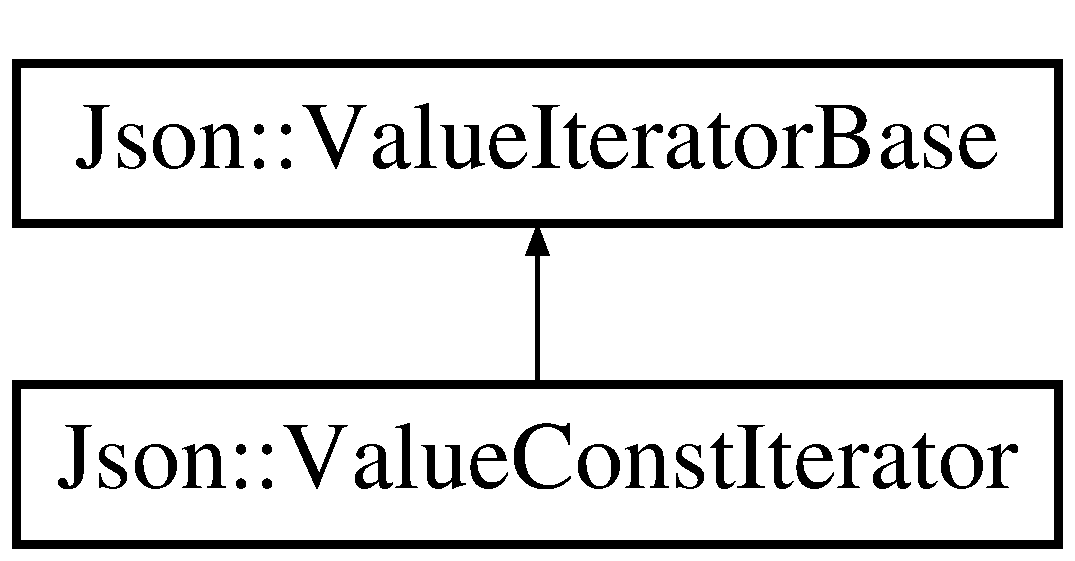
\includegraphics[height=2.000000cm]{class_json_1_1_value_const_iterator}
\end{center}
\end{figure}
\subsection*{Public Types}
\begin{DoxyCompactItemize}
\item 
\hypertarget{class_json_1_1_value_const_iterator_a8685219d214dbd2b763357ae94fb0f27}{typedef unsigned int {\bfseries size\-\_\-t}}\label{class_json_1_1_value_const_iterator_a8685219d214dbd2b763357ae94fb0f27}

\item 
\hypertarget{class_json_1_1_value_const_iterator_a32b36aa9d76e2b48ca74fb6e1979a95a}{typedef int {\bfseries difference\-\_\-type}}\label{class_json_1_1_value_const_iterator_a32b36aa9d76e2b48ca74fb6e1979a95a}

\item 
\hypertarget{class_json_1_1_value_const_iterator_aa9b05c6a37cd352ea1ee6e13b816f709}{typedef const \hyperlink{class_json_1_1_value}{Value} \& {\bfseries reference}}\label{class_json_1_1_value_const_iterator_aa9b05c6a37cd352ea1ee6e13b816f709}

\item 
\hypertarget{class_json_1_1_value_const_iterator_a400136bd8bc09e9fddec0785fa2cff14}{typedef const \hyperlink{class_json_1_1_value}{Value} $\ast$ {\bfseries pointer}}\label{class_json_1_1_value_const_iterator_a400136bd8bc09e9fddec0785fa2cff14}

\item 
\hypertarget{class_json_1_1_value_const_iterator_a0c2e33e7eb5a80dd8709fb28ece83933}{typedef \hyperlink{class_json_1_1_value_const_iterator}{Value\-Const\-Iterator} {\bfseries Self\-Type}}\label{class_json_1_1_value_const_iterator_a0c2e33e7eb5a80dd8709fb28ece83933}

\end{DoxyCompactItemize}
\subsection*{Public Member Functions}
\begin{DoxyCompactItemize}
\item 
\hypertarget{class_json_1_1_value_const_iterator_ad1b1c11f8d7fb22d4d3c231915f2b15b}{\hyperlink{class_json_1_1_value_iterator_base}{Self\-Type} \& {\bfseries operator=} (const \hyperlink{class_json_1_1_value_iterator_base}{Value\-Iterator\-Base} \&other)}\label{class_json_1_1_value_const_iterator_ad1b1c11f8d7fb22d4d3c231915f2b15b}

\item 
\hypertarget{class_json_1_1_value_const_iterator_ab3f0c2edbfc8f7d60645f3d597d05e28}{\hyperlink{class_json_1_1_value_iterator_base}{Self\-Type} {\bfseries operator++} (int)}\label{class_json_1_1_value_const_iterator_ab3f0c2edbfc8f7d60645f3d597d05e28}

\item 
\hypertarget{class_json_1_1_value_const_iterator_a94935961e9331c6f7b907b05ec8df75e}{\hyperlink{class_json_1_1_value_iterator_base}{Self\-Type} {\bfseries operator-\/-\/} (int)}\label{class_json_1_1_value_const_iterator_a94935961e9331c6f7b907b05ec8df75e}

\item 
\hypertarget{class_json_1_1_value_const_iterator_a31415e44e44e56fb2bfda7e8bb784646}{\hyperlink{class_json_1_1_value_iterator_base}{Self\-Type} \& {\bfseries operator-\/-\/} ()}\label{class_json_1_1_value_const_iterator_a31415e44e44e56fb2bfda7e8bb784646}

\item 
\hypertarget{class_json_1_1_value_const_iterator_a2cfe2f7a94a688186efdafb1b181c319}{\hyperlink{class_json_1_1_value_iterator_base}{Self\-Type} \& {\bfseries operator++} ()}\label{class_json_1_1_value_const_iterator_a2cfe2f7a94a688186efdafb1b181c319}

\item 
\hypertarget{class_json_1_1_value_const_iterator_aeb44153d71c61ac9397a84d5ecc244c5}{\hyperlink{class_json_1_1_value}{reference} {\bfseries operator$\ast$} () const }\label{class_json_1_1_value_const_iterator_aeb44153d71c61ac9397a84d5ecc244c5}

\end{DoxyCompactItemize}
\subsection*{Private Member Functions}
\begin{DoxyCompactItemize}
\item 
\hypertarget{class_json_1_1_value_const_iterator_aa0a87edf5f1097f91dca5f2a389c4abd}{{\bfseries Value\-Const\-Iterator} (const Value\-::\-Object\-Values\-::iterator \&current)}\label{class_json_1_1_value_const_iterator_aa0a87edf5f1097f91dca5f2a389c4abd}

\end{DoxyCompactItemize}
\subsection*{Friends}
\begin{DoxyCompactItemize}
\item 
\hypertarget{class_json_1_1_value_const_iterator_aeceedf6e1a7d48a588516ce2b1983d6f}{class {\bfseries Value}}\label{class_json_1_1_value_const_iterator_aeceedf6e1a7d48a588516ce2b1983d6f}

\end{DoxyCompactItemize}
\subsection*{Additional Inherited Members}


\subsection{Detailed Description}
const iterator for object and array value. 



The documentation for this class was generated from the following files\-:\begin{DoxyCompactItemize}
\item 
/\-Users/\-Alex/github/\-A\-W\-E\-Media\-Center/\-Code/libs/json/json.\-h\item 
/\-Users/\-Alex/github/\-A\-W\-E\-Media\-Center/\-Code/libs/json/jsoncpp.\-cpp\end{DoxyCompactItemize}

\hypertarget{class_json_1_1_value_iterator}{\section{Json\-:\-:Value\-Iterator Class Reference}
\label{class_json_1_1_value_iterator}\index{Json\-::\-Value\-Iterator@{Json\-::\-Value\-Iterator}}
}


Iterator for object and array value.  




{\ttfamily \#include $<$json.\-h$>$}

Inheritance diagram for Json\-:\-:Value\-Iterator\-:\begin{figure}[H]
\begin{center}
\leavevmode
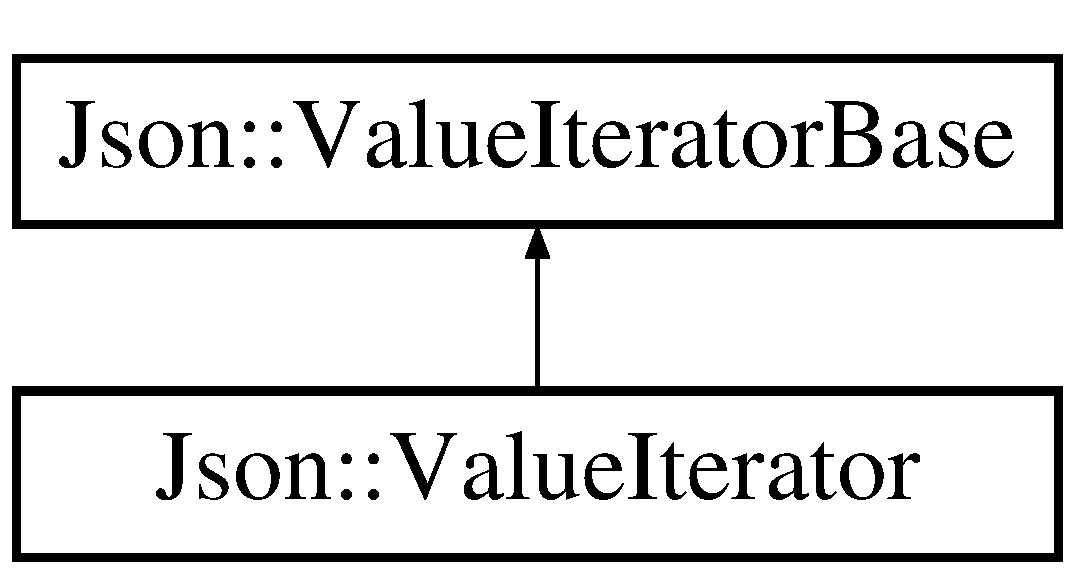
\includegraphics[height=2.000000cm]{class_json_1_1_value_iterator}
\end{center}
\end{figure}
\subsection*{Public Types}
\begin{DoxyCompactItemize}
\item 
\hypertarget{class_json_1_1_value_iterator_a308b8932ffc83eaa9d12dadd5c11a7dd}{typedef unsigned int {\bfseries size\-\_\-t}}\label{class_json_1_1_value_iterator_a308b8932ffc83eaa9d12dadd5c11a7dd}

\item 
\hypertarget{class_json_1_1_value_iterator_a2be1a9aa60bbfc8812e9dd1a7f1a8786}{typedef int {\bfseries difference\-\_\-type}}\label{class_json_1_1_value_iterator_a2be1a9aa60bbfc8812e9dd1a7f1a8786}

\item 
\hypertarget{class_json_1_1_value_iterator_ae87929b4567aa00372cf602c43b57160}{typedef \hyperlink{class_json_1_1_value}{Value} \& {\bfseries reference}}\label{class_json_1_1_value_iterator_ae87929b4567aa00372cf602c43b57160}

\item 
\hypertarget{class_json_1_1_value_iterator_acec45feb1ef1f3bf81240157d06d5432}{typedef \hyperlink{class_json_1_1_value}{Value} $\ast$ {\bfseries pointer}}\label{class_json_1_1_value_iterator_acec45feb1ef1f3bf81240157d06d5432}

\item 
\hypertarget{class_json_1_1_value_iterator_a23357670fdad61792670d86f62db7e16}{typedef \hyperlink{class_json_1_1_value_iterator}{Value\-Iterator} {\bfseries Self\-Type}}\label{class_json_1_1_value_iterator_a23357670fdad61792670d86f62db7e16}

\end{DoxyCompactItemize}
\subsection*{Public Member Functions}
\begin{DoxyCompactItemize}
\item 
\hypertarget{class_json_1_1_value_iterator_aa85aa208670891670392259efa0143bb}{{\bfseries Value\-Iterator} (const \hyperlink{class_json_1_1_value_const_iterator}{Value\-Const\-Iterator} \&other)}\label{class_json_1_1_value_iterator_aa85aa208670891670392259efa0143bb}

\item 
\hypertarget{class_json_1_1_value_iterator_a7d5e58a9a4a553968acdf3064b39d21c}{{\bfseries Value\-Iterator} (const \hyperlink{class_json_1_1_value_iterator}{Value\-Iterator} \&other)}\label{class_json_1_1_value_iterator_a7d5e58a9a4a553968acdf3064b39d21c}

\item 
\hypertarget{class_json_1_1_value_iterator_a8e23312b1db874f7e403fd7e76611bdc}{\hyperlink{class_json_1_1_value_iterator_base}{Self\-Type} \& {\bfseries operator=} (const \hyperlink{class_json_1_1_value_iterator_base}{Self\-Type} \&other)}\label{class_json_1_1_value_iterator_a8e23312b1db874f7e403fd7e76611bdc}

\item 
\hypertarget{class_json_1_1_value_iterator_abcf4ddd994a010742cd4a436d65acd08}{\hyperlink{class_json_1_1_value_iterator_base}{Self\-Type} {\bfseries operator++} (int)}\label{class_json_1_1_value_iterator_abcf4ddd994a010742cd4a436d65acd08}

\item 
\hypertarget{class_json_1_1_value_iterator_a06d6a29d96caf6af324a53973159e12b}{\hyperlink{class_json_1_1_value_iterator_base}{Self\-Type} {\bfseries operator-\/-\/} (int)}\label{class_json_1_1_value_iterator_a06d6a29d96caf6af324a53973159e12b}

\item 
\hypertarget{class_json_1_1_value_iterator_a811302a868518a0995a9def955df5720}{\hyperlink{class_json_1_1_value_iterator_base}{Self\-Type} \& {\bfseries operator-\/-\/} ()}\label{class_json_1_1_value_iterator_a811302a868518a0995a9def955df5720}

\item 
\hypertarget{class_json_1_1_value_iterator_a92146c46f8249e2b2d12869e70cd4cee}{\hyperlink{class_json_1_1_value_iterator_base}{Self\-Type} \& {\bfseries operator++} ()}\label{class_json_1_1_value_iterator_a92146c46f8249e2b2d12869e70cd4cee}

\item 
\hypertarget{class_json_1_1_value_iterator_aaa5be3457eedf0526a03b8a3b4c7c0a0}{\hyperlink{class_json_1_1_value}{reference} {\bfseries operator$\ast$} () const }\label{class_json_1_1_value_iterator_aaa5be3457eedf0526a03b8a3b4c7c0a0}

\end{DoxyCompactItemize}
\subsection*{Private Member Functions}
\begin{DoxyCompactItemize}
\item 
\hypertarget{class_json_1_1_value_iterator_afb06ea21add440c78c27dc49570460a5}{{\bfseries Value\-Iterator} (const Value\-::\-Object\-Values\-::iterator \&current)}\label{class_json_1_1_value_iterator_afb06ea21add440c78c27dc49570460a5}

\end{DoxyCompactItemize}
\subsection*{Friends}
\begin{DoxyCompactItemize}
\item 
\hypertarget{class_json_1_1_value_iterator_aeceedf6e1a7d48a588516ce2b1983d6f}{class {\bfseries Value}}\label{class_json_1_1_value_iterator_aeceedf6e1a7d48a588516ce2b1983d6f}

\end{DoxyCompactItemize}
\subsection*{Additional Inherited Members}


\subsection{Detailed Description}
Iterator for object and array value. 

The documentation for this class was generated from the following files\-:\begin{DoxyCompactItemize}
\item 
/\-Users/\-Alex/github/\-A\-W\-E\-Media\-Center/\-Code/libs/json/json.\-h\item 
/\-Users/\-Alex/github/\-A\-W\-E\-Media\-Center/\-Code/libs/json/jsoncpp.\-cpp\end{DoxyCompactItemize}

\hypertarget{class_json_1_1_value_iterator_base}{\section{Json\-:\-:Value\-Iterator\-Base Class Reference}
\label{class_json_1_1_value_iterator_base}\index{Json\-::\-Value\-Iterator\-Base@{Json\-::\-Value\-Iterator\-Base}}
}


base class for \hyperlink{class_json_1_1_value}{Value} iterators.  




{\ttfamily \#include $<$json.\-h$>$}

Inheritance diagram for Json\-:\-:Value\-Iterator\-Base\-:\begin{figure}[H]
\begin{center}
\leavevmode
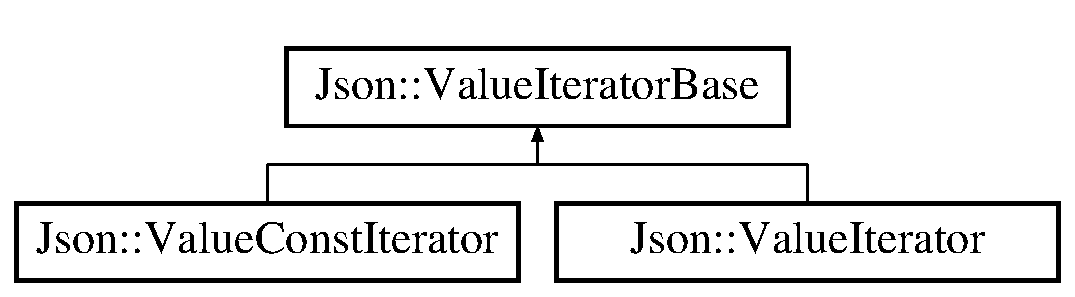
\includegraphics[height=2.000000cm]{class_json_1_1_value_iterator_base}
\end{center}
\end{figure}
\subsection*{Public Types}
\begin{DoxyCompactItemize}
\item 
\hypertarget{class_json_1_1_value_iterator_base_a9d3a3c7ce5cdefe23cb486239cf07bb5}{typedef unsigned int {\bfseries size\-\_\-t}}\label{class_json_1_1_value_iterator_base_a9d3a3c7ce5cdefe23cb486239cf07bb5}

\item 
\hypertarget{class_json_1_1_value_iterator_base_a4e44bf8cbd17ec8d6e2c185904a15ebd}{typedef int {\bfseries difference\-\_\-type}}\label{class_json_1_1_value_iterator_base_a4e44bf8cbd17ec8d6e2c185904a15ebd}

\item 
\hypertarget{class_json_1_1_value_iterator_base_a9d2a940d03ea06d20d972f41a89149ee}{typedef \hyperlink{class_json_1_1_value_iterator_base}{Value\-Iterator\-Base} {\bfseries Self\-Type}}\label{class_json_1_1_value_iterator_base_a9d2a940d03ea06d20d972f41a89149ee}

\end{DoxyCompactItemize}
\subsection*{Public Member Functions}
\begin{DoxyCompactItemize}
\item 
\hypertarget{class_json_1_1_value_iterator_base_a640e990e5f03a96fd650122a2906f59d}{{\bfseries Value\-Iterator\-Base} (const Value\-::\-Object\-Values\-::iterator \&current)}\label{class_json_1_1_value_iterator_base_a640e990e5f03a96fd650122a2906f59d}

\item 
\hypertarget{class_json_1_1_value_iterator_base_afc656672ac28502f640ade32c38c1b56}{bool {\bfseries operator==} (const \hyperlink{class_json_1_1_value_iterator_base}{Self\-Type} \&other) const }\label{class_json_1_1_value_iterator_base_afc656672ac28502f640ade32c38c1b56}

\item 
\hypertarget{class_json_1_1_value_iterator_base_a18c2dd42e0bb989ace141bfe9de52792}{bool {\bfseries operator!=} (const \hyperlink{class_json_1_1_value_iterator_base}{Self\-Type} \&other) const }\label{class_json_1_1_value_iterator_base_a18c2dd42e0bb989ace141bfe9de52792}

\item 
\hypertarget{class_json_1_1_value_iterator_base_ab786787fcad68ca5e8745aaf520fa17f}{difference\-\_\-type {\bfseries operator-\/} (const \hyperlink{class_json_1_1_value_iterator_base}{Self\-Type} \&other) const }\label{class_json_1_1_value_iterator_base_ab786787fcad68ca5e8745aaf520fa17f}

\item 
\hypertarget{class_json_1_1_value_iterator_base_aa2ff5e79fc96acd4c3cd288e92614fc7}{\hyperlink{class_json_1_1_value}{Value} \hyperlink{class_json_1_1_value_iterator_base_aa2ff5e79fc96acd4c3cd288e92614fc7}{key} () const }\label{class_json_1_1_value_iterator_base_aa2ff5e79fc96acd4c3cd288e92614fc7}

\begin{DoxyCompactList}\small\item\em Return either the index or the member name of the referenced value as a \hyperlink{class_json_1_1_value}{Value}. \end{DoxyCompactList}\item 
\hypertarget{class_json_1_1_value_iterator_base_aa90591f5f7f8d2f06cc4605816b53738}{U\-Int \hyperlink{class_json_1_1_value_iterator_base_aa90591f5f7f8d2f06cc4605816b53738}{index} () const }\label{class_json_1_1_value_iterator_base_aa90591f5f7f8d2f06cc4605816b53738}

\begin{DoxyCompactList}\small\item\em Return the index of the referenced \hyperlink{class_json_1_1_value}{Value}. -\/1 if it is not an array\-Value. \end{DoxyCompactList}\item 
\hypertarget{class_json_1_1_value_iterator_base_a83768d87c608c8d1133de8721eefc31b}{const char $\ast$ \hyperlink{class_json_1_1_value_iterator_base_a83768d87c608c8d1133de8721eefc31b}{member\-Name} () const }\label{class_json_1_1_value_iterator_base_a83768d87c608c8d1133de8721eefc31b}

\begin{DoxyCompactList}\small\item\em Return the member name of the referenced \hyperlink{class_json_1_1_value}{Value}. \char`\"{}\char`\"{} if it is not an object\-Value. \end{DoxyCompactList}\end{DoxyCompactItemize}
\subsection*{Protected Member Functions}
\begin{DoxyCompactItemize}
\item 
\hypertarget{class_json_1_1_value_iterator_base_a40a20c65abc423a26e3aae68d9a0525c}{\hyperlink{class_json_1_1_value}{Value} \& {\bfseries deref} () const }\label{class_json_1_1_value_iterator_base_a40a20c65abc423a26e3aae68d9a0525c}

\item 
\hypertarget{class_json_1_1_value_iterator_base_afe58f9534e1fd2033419fd9fe244551e}{void {\bfseries increment} ()}\label{class_json_1_1_value_iterator_base_afe58f9534e1fd2033419fd9fe244551e}

\item 
\hypertarget{class_json_1_1_value_iterator_base_affc8cf5ff54a9f432cc693362c153fa6}{void {\bfseries decrement} ()}\label{class_json_1_1_value_iterator_base_affc8cf5ff54a9f432cc693362c153fa6}

\item 
\hypertarget{class_json_1_1_value_iterator_base_ad6c553b249e89e3dc9933e100ccbe064}{difference\-\_\-type {\bfseries compute\-Distance} (const \hyperlink{class_json_1_1_value_iterator_base}{Self\-Type} \&other) const }\label{class_json_1_1_value_iterator_base_ad6c553b249e89e3dc9933e100ccbe064}

\item 
\hypertarget{class_json_1_1_value_iterator_base_a21820d6ee564e541bd118b21e4741962}{bool {\bfseries is\-Equal} (const \hyperlink{class_json_1_1_value_iterator_base}{Self\-Type} \&other) const }\label{class_json_1_1_value_iterator_base_a21820d6ee564e541bd118b21e4741962}

\item 
\hypertarget{class_json_1_1_value_iterator_base_a496e6aba44808433ec5858c178be5719}{void {\bfseries copy} (const \hyperlink{class_json_1_1_value_iterator_base}{Self\-Type} \&other)}\label{class_json_1_1_value_iterator_base_a496e6aba44808433ec5858c178be5719}

\end{DoxyCompactItemize}


\subsection{Detailed Description}
base class for \hyperlink{class_json_1_1_value}{Value} iterators. 



The documentation for this class was generated from the following files\-:\begin{DoxyCompactItemize}
\item 
/\-Users/\-Alex/github/\-A\-W\-E\-Media\-Center/\-Code/libs/json/json.\-h\item 
/\-Users/\-Alex/github/\-A\-W\-E\-Media\-Center/\-Code/libs/json/jsoncpp.\-cpp\end{DoxyCompactItemize}

\hypertarget{class_json_1_1_writer}{\section{Json\-:\-:Writer Class Reference}
\label{class_json_1_1_writer}\index{Json\-::\-Writer@{Json\-::\-Writer}}
}


Abstract class for writers.  




{\ttfamily \#include $<$json.\-h$>$}

Inheritance diagram for Json\-:\-:Writer\-:\begin{figure}[H]
\begin{center}
\leavevmode
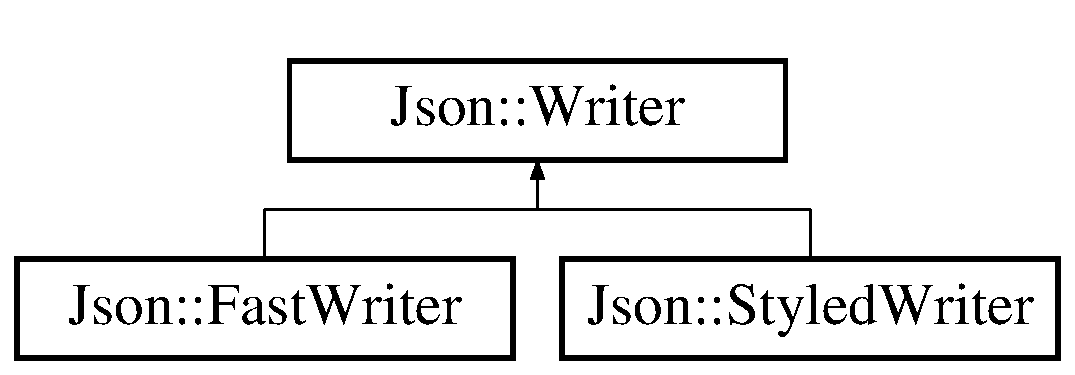
\includegraphics[height=2.000000cm]{class_json_1_1_writer}
\end{center}
\end{figure}
\subsection*{Public Member Functions}
\begin{DoxyCompactItemize}
\item 
\hypertarget{class_json_1_1_writer_a7b2273a4ffd6f32b369ac8a53b7b5a0d}{virtual std\-::string {\bfseries write} (const \hyperlink{class_json_1_1_value}{Value} \&root)=0}\label{class_json_1_1_writer_a7b2273a4ffd6f32b369ac8a53b7b5a0d}

\end{DoxyCompactItemize}


\subsection{Detailed Description}
Abstract class for writers. 

The documentation for this class was generated from the following files\-:\begin{DoxyCompactItemize}
\item 
/\-Users/\-Alex/github/\-A\-W\-E\-Media\-Center/\-Code/libs/json/json.\-h\item 
/\-Users/\-Alex/github/\-A\-W\-E\-Media\-Center/\-Code/libs/json/jsoncpp.\-cpp\end{DoxyCompactItemize}

%--- End generated contents ---

% Index
\newpage
\phantomsection
\addcontentsline{toc}{chapter}{Index}
\printindex

\end{document}
